%&preformat-present
%make clean; make presentation
\newif\ifpresentation % Условие, проверяющее, что документ --- презентация
\presentationtrue
\documentclass[10pt, xcolor={dvipsnames, table, hyperref},aspectratio=169]{beamer}


%%%\setbeameroption{hide notes} % Only slides
%%%\setbeameroption{show only notes} % Only notes

%Uncomment four lines below if notes are needed. 
% \usepackage{pgfpages}
% \setbeameroption{show notes on second screen=right} % Both
% \setbeamertemplate{note page}{\pagecolor{yellow!5}\insertnote}\usepackage{palatino}
% \newcommand*{\HANDOUT}{}

%%%%%%%%%%%%%%%%%%%%%%%%%%%%%%%%%%%%%%%%%%%%%%%%%%%%%%%%%%%%%%%%%%%%%%%%%%%%%%%%
%%%% Файл упрощённых настроек шаблона, общих для диссертации и автореферата %%%%
%%%%%%%%%%%%%%%%%%%%%%%%%%%%%%%%%%%%%%%%%%%%%%%%%%%%%%%%%%%%%%%%%%%%%%%%%%%%%%%%

%%% Режим черновика %%%
\makeatletter
\@ifundefined{c@draft}{
  \newcounter{draft}
  \setcounter{draft}{0}  % 0 --- чистовик (максимальное соблюдение ГОСТ)
                         % 1 --- черновик (отклонения от ГОСТ, но быстрая
                         %       сборка итоговых PDF)
}{}
\makeatother

%%% Пометки в тексте %%%
\makeatletter
\@ifundefined{c@showmarkup}{
  \newcounter{showmarkup}
  \setcounter{showmarkup}{0}  % 0 --- скрыть пометки
                              % 1 --- показывать пометки
}{}
\makeatother

%%% Использование в pdflatex шрифтов не по-умолчанию %%%
\makeatletter
\@ifundefined{c@usealtfont}{
  \newcounter{usealtfont}
  \setcounter{usealtfont}{1}    % 0 --- шрифты на базе Computer Modern
                                % 1 --- использовать пакет pscyr, при его
                                %       наличии
                                % 2 --- использовать пакет XCharter, при наличии
                                %       подходящей версии
}{}
\makeatother

%%% Использование в xelatex и lualatex семейств шрифтов %%%
\makeatletter
\@ifundefined{c@fontfamily}{
  \newcounter{fontfamily}
  \setcounter{fontfamily}{1}  % 0 --- CMU семейство. Используется как fallback;
                              % 1 --- Шрифты от MS (Times New Roman и компания)
                              % 2 --- Семейство Liberation
}{}
\makeatother

%%% Библиография %%%
\makeatletter
\@ifundefined{c@bibliosel}{
  \newcounter{bibliosel}
  \setcounter{bibliosel}{1}   % 0 --- встроенная реализация с загрузкой файла
                              %       через движок bibtex8;
                              % 1 --- реализация пакетом biblatex через движок
                              %       biber
}{}
\makeatother

%%% Вывод типов ссылок в библиографии %%%
\makeatletter
\@ifundefined{c@mediadisplay}{
  \newcounter{mediadisplay}
  \setcounter{mediadisplay}{0}   % 0 --- не делать ничего; надписи [Текст] и
                                 %       [Эл. ресурс] будут выводиться только в ссылках с
                                 %       заполненным полем `media`;
                                 % 1 --- автоматически добавлять надпись [Текст] к ссылкам с
                                 %       незаполненным полем `media`; таким образом, у всех
                                 %       источников будет указан тип, что соответствует
                                 %       требованиям ГОСТ
                                 % 2 --- автоматически удалять надписи [Текст], [Эл. Ресурс] и др.;
                                 %       не соответствует ГОСТ
                                 % 3 --- автоматически удалять надпись [Текст];
                                 %       не соответствует ГОСТ
                                 % 4 --- автоматически удалять надпись [Эл. Ресурс];
                                 %       не соответствует ГОСТ
}{}
\makeatother

%%% Предкомпиляция tikz рисунков для ускорения работы %%%
\makeatletter
\@ifundefined{c@imgprecompile}{
  \newcounter{imgprecompile}
  \setcounter{imgprecompile}{0}   % 0 --- без предкомпиляции;
                                  % 1 --- пользоваться предварительно
                                  %       скомпилированными pdf вместо генерации
                                  %       заново из tikz
}{}
\makeatother
               % Общие настройки шаблона

% \usepackage{xpatch} %AKSh
%%% Проверка используемого TeX-движка %%%
\newif\ifxetexorluatex   % определяем новый условный оператор (http://tex.stackexchange.com/a/47579)
\ifxetex
    \xetexorluatextrue
\else
    \ifluatex
        \xetexorluatextrue
    \else
        \xetexorluatexfalse
    \fi
\fi

\newif\ifsynopsis           % Условие, проверяющее, что документ --- автореферат

\usepackage{etoolbox}[2015/08/02]   % Для продвинутой проверки разных условий
\providebool{presentation}

\usepackage{comment}    % Позволяет убирать блоки текста (добавляет
                        % окружение comment и команду \excludecomment)

                       

%%% Поля и разметка страницы %%%
\usepackage{pdflscape}  % Для включения альбомных страниц
\usepackage{geometry}   % Для последующего задания полей

%%% Математические пакеты %%%
\usepackage{amsthm,amsmath,amscd}   % Математические дополнения от AMS
\usepackage{amsfonts,amssymb}       % Математические дополнения от AMS
\usepackage{mathtools}              % Добавляет окружение multlined
\usepackage{xfrac}                  % Красивые дроби
\usepackage[
    locale = DE,
    list-separator       = {;\,},
    list-final-separator = {;\,},
    list-pair-separator  = {;\,},
    list-units           = single,
    range-units          = single,
    range-phrase={\text{\ensuremath{-}}},
    % quotient-mode        = fraction, % красивые дроби могут не соответствовать ГОСТ
    fraction-function    = \sfrac,
    separate-uncertainty,
    ]{siunitx}                      % Размерности SI
\sisetup{inter-unit-product = \ensuremath{{}\cdot{}}}



%Пользовательские насройки и доппакеты
\DeclareMathOperator{\erfc}{erfc} %Added by AkSh 1.10.2020
\usepackage{tabularx} %Added by Aksh 2.10.2020
\usepackage{float}

% Кириллица в нумерации subequations
% Для правильной работы требуется выполнение сразу после загрузки пакетов
\patchcmd{\subequations}{\def\theequation{\theparentequation\alph{equation}}}
{\def\theequation{\theparentequation\asbuk{equation}}}
{\typeout{subequations patched}}{\typeout{subequations not patched}}

%%%% Установки для размера шрифта 14 pt %%%%
%% Формирование переменных и констант для сравнения (один раз для всех подключаемых файлов)%%
%% должно располагаться до вызова пакета fontspec или polyglossia, потому что они сбивают его работу
\newlength{\curtextsize}
\newlength{\bigtextsize}
\setlength{\bigtextsize}{13.9pt}

\makeatletter
%\show\f@size    % неплохо для отслеживания, но вызывает стопорение процесса,
                 % если документ компилируется без команды  -interaction=nonstopmode
\setlength{\curtextsize}{\f@size pt}
\makeatother

%%% Кодировки и шрифты %%%
\ifxetexorluatex
    \ifpresentation
        \providecommand*\autodot{} % quick fix for polyglossia 1.50
    \fi
    \PassOptionsToPackage{no-math}{fontspec}    % https://tex.stackexchange.com/a/26295/104425
    \usepackage{polyglossia}[2014/05/21]        % Поддержка многоязычности
                                        % (fontspec подгружается автоматически)
\else
   %%% Решение проблемы копирования текста в буфер кракозябрами
    \ifnumequal{\value{usealtfont}}{0}{}{
        \input glyphtounicode.tex
        \input glyphtounicode-cmr.tex %from pdfx package
        \pdfgentounicode=1
    }
    \usepackage{cmap}   % Улучшенный поиск русских слов в полученном pdf-файле
    \ifnumequal{\value{usealtfont}}{2}{}{
        \defaulthyphenchar=127  % Если стоит до fontenc, то переносы
                                % не впишутся в выделяемый текст при
                                % копировании его в буфер обмена
    }
    \usepackage{textcomp}
    \usepackage[T1,T2A]{fontenc}                    % Поддержка русских букв
    \ifnumequal{\value{usealtfont}}{1}{% Используется pscyr, при наличии
        \IfFileExists{pscyr.sty}{\usepackage{pscyr}}{}  % Подключение pscyr
    }{}
    \usepackage[utf8]{inputenc}[2014/04/30]         % Кодировка utf8
    \usepackage[english,russian]{babel}[2014/03/24]% Языки: русский, английский
    \makeatletter\AtBeginDocument{\let\@elt\relax}\makeatother % babel 3.40 fix
    \ifnumequal{\value{usealtfont}}{2}{
        % http://dxdy.ru/post1238763.html#p1238763
        \usepackage[scaled=0.914]{XCharter}[2017/12/19] % Подключение русифицированных шрифтов XCharter
        \usepackage[charter, vvarbb, scaled=1.048]{newtxmath}[2017/12/14]
        \ifpresentation
        \else
            \setDisplayskipStretch{-0.078}
        \fi
    }{}
\fi

%%% Оформление абзацев %%%
\ifpresentation
\else
    \indentafterchapter     % Красная строка после заголовков типа chapter
    \usepackage{indentfirst}
\fi

%%% Цвета %%%
\ifpresentation
\else
    \usepackage[dvipsnames, table, hyperref]{xcolor} % Совместимо с tikz
\fi

%%% Таблицы %%%
\usepackage{longtable,ltcaption} % Длинные таблицы
\usepackage{multirow,makecell}   % Улучшенное форматирование таблиц
\usepackage{tabu, tabulary}      % таблицы с автоматически подбирающейся
                                 % шириной столбцов (tabu обязательно
                                 % до hyperref вызывать)
\usepackage{threeparttable}      % автоматический подгон ширины подписи таблицы

%%% Общее форматирование
\usepackage{soulutf8}% Поддержка переносоустойчивых подчёркиваний и зачёркиваний
\usepackage{icomma}  % Запятая в десятичных дробях

%%% Оптимизация расстановки переносов и длины последней строки абзаца
\IfFileExists{impnattypo.sty}{% проверка установленности пакета impnattypo
    \ifluatex
        \ifnumequal{\value{draft}}{1}{% Черновик
            \usepackage[hyphenation, lastparline, nosingleletter, homeoarchy,
            rivers, draft]{impnattypo}
        }{% Чистовик
            \usepackage[hyphenation, lastparline, nosingleletter]{impnattypo}
        }
    \else
        \usepackage[hyphenation, lastparline]{impnattypo}
    \fi
}{}

%% Векторная графика

\usepackage{tikz}                   % Продвинутый пакет векторной графики
\usetikzlibrary{chains}             % Для примера tikz рисунка
\usetikzlibrary{shapes.geometric}   % Для примера tikz рисунка
\usetikzlibrary{shapes.symbols}     % Для примера tikz рисунка
\usetikzlibrary{arrows}             % Для примера tikz рисунка

%%% Гиперссылки %%%
\usepackage{hyperref}[2012/11/06]

%%% Изображения %%%
\usepackage{graphicx}[2014/04/25]   % Подключаем пакет работы с графикой
\usepackage[labelfont=bf]{caption}                % Подписи рисунков и таблиц %labelfont=bf Added by AKSh
\usepackage{subcaption}             % Подписи подрисунков и подтаблиц
\usepackage{pdfpages}               % Добавление внешних pdf файлов

%%% Счётчики %%%
\usepackage{aliascnt}
\usepackage[figure,table]{totalcount}   % Счётчик рисунков и таблиц
\usepackage{totcount}   % Пакет создания счётчиков на основе последнего номера
                        % подсчитываемого элемента (может требовать дважды
                        % компилировать документ)
\usepackage{totpages}   % Счётчик страниц, совместимый с hyperref (ссылается
                        % на номер последней страницы). Желательно ставить
                        % последним пакетом в преамбуле

%%% Продвинутое управление групповыми ссылками (пока только формулами) %%%
\ifpresentation
\else
    \usepackage[russian]{cleveref} % cleveref имеет сложности со считыванием
    % языка из babel. Такое решение русификации вывода выбрано вместо
    % определения в documentclass из опасности что-то лишнее передать во все
    % остальные пакеты, включая библиографию.

    % Добавление возможности использования пробелов в \labelcref
    % https://tex.stackexchange.com/a/340502/104425
    \usepackage{kvsetkeys}
    \makeatletter
    \let\org@@cref\@cref
    \renewcommand*{\@cref}[2]{%
        \edef\process@me{%
            \noexpand\org@@cref{#1}{\zap@space#2 \@empty}%
        }\process@me
    }
    \makeatother
\fi

\usepackage{placeins} % для \FloatBarrier

\ifnumequal{\value{draft}}{1}{% Черновик
    \usepackage[firstpage]{draftwatermark}
    \SetWatermarkText{DRAFT}
    \SetWatermarkFontSize{14pt}
    \SetWatermarkScale{15}
    \SetWatermarkAngle{45}
}{}

%%% Цитата, не приводимая в автореферате:
% возможно, актуальна только для biblatex
%\newcommand{\citeinsynopsis}[1]{\ifsynopsis\else ~\cite{#1} \fi}

% если текущий процесс запущен библиотекой tikz-external, то прекомпиляция должна быть включена
\ifdefined\tikzexternalrealjob
    \setcounter{imgprecompile}{1}
\fi

\ifnumequal{\value{imgprecompile}}{1}{% Только если у нас включена предкомпиляция
    \usetikzlibrary{external}   % подключение возможности предкомпиляции
    \tikzexternalize[prefix=images/cache/,optimize command away=\includepdf] % activate! % здесь можно указать отдельную папку для скомпилированных файлов
    \ifxetex
        \tikzset{external/up to date check={diff}}
    \fi
}{}
            % Пакеты общие для диссертации и автореферата
%%% Основные сведения %%%
\newcommand{\thesisAuthorLastName}{Шайтан}
\newcommand{\thesisAuthorOtherNames}{Алексей Константинович}
\newcommand{\thesisAuthorInitials}{А.\,К.}
\newcommand{\thesisAuthor}             % Диссертация, ФИО автора
{%
    \texorpdfstring{% \texorpdfstring takes two arguments and uses the first for (La)TeX and the second for pdf
        \thesisAuthorLastName~\thesisAuthorOtherNames% так будет отображаться на титульном листе или в тексте, где будет использоваться переменная
    }{%
        \thesisAuthorLastName, \thesisAuthorOtherNames% эта запись для свойств pdf-файла. В таком виде, если pdf будет обработан программами для сбора библиографических сведений, будет правильно представлена фамилия.
    }
}
\newcommand{\thesisAuthorShort}        % Диссертация, ФИО автора инициалами
{\thesisAuthorInitials~\thesisAuthorLastName}
\newcommand{\thesisUdk}                % Диссертация, УДК
{577.3}
\newcommand{\thesisTitle}              % Диссертация, название
{Интегративное моделирование структуры и динамики биомакромолекулярных комплексов}
\newcommand{\thesisSpecialtyNumber}    % Диссертация, специальность, номер
{03.01.09}
\newcommand{\thesisSpecialtyTitle}     % Диссертация, специальность, название (название взято с сайта ВАК для примера)
{Математическая биология, биоинформатика}
%% \newcommand{\thesisSpecialtyTwoNumber} % Диссертация, вторая специальность, номер
%% {\fixme{XX.XX.XX}}
%% \newcommand{\thesisSpecialtyTwoTitle}  % Диссертация, вторая специальность, название
%% {\fixme{Теория и~методика физического воспитания, спортивной тренировки,
%% оздоровительной и~адаптивной физической культуры}}
\newcommand{\thesisDegree}             % Диссертация, ученая степень
{доктора физико-математических наук}
\newcommand{\thesisDegreeShort}        % Диссертация, ученая степень, краткая запись
{докт. физ.-мат. наук}
\newcommand{\thesisCity}               % Диссертация, город написания диссертации
{Москва}
\newcommand{\thesisYear}               % Диссертация, год написания диссертации
{\the\year}
\newcommand{\thesisOrganization}       % Диссертация, организация
{МОСКОВСКИЙ ГОСУДАРСТВЕННЫЙ УНИВЕРСИТЕТ \\ имени М.В.ЛОМОНОСОВА\\ БИОЛОГИЧЕСКИЙ ФАКУЛЬТЕТ}
\newcommand{\thesisOrganizationShort}  % Диссертация, краткое название организации для доклада
{МГУ им. М.В.Ломоносова}

\newcommand{\thesisInOrganization}     % Диссертация, организация в предложном падеже: Работа выполнена в ...
{кафедре биоинженерии биологического факультета МГУ имени М.В.Ломоносова}

%% \newcommand{\supervisorDead}{}           % Рисовать рамку вокруг фамилии
\newcommand{\supervisorFio}              % Научный руководитель, ФИО
{Кирпичников Михаил Петрович}
\newcommand{\supervisorRegalia}          % Научный руководитель, регалии
{д-р~биол. наук, академик РАН}
\newcommand{\supervisorFioShort}         % Научный руководитель, ФИО
{М.\,П.~Кирпичников}
\newcommand{\supervisorRegaliaShort}     % Научный руководитель, регалии
{академик РАН,~д.б.н.}

%% \newcommand{\supervisorTwoDead}{}        % Рисовать рамку вокруг фамилии
%% \newcommand{\supervisorTwoFio}           % Второй научный руководитель, ФИО
%% {\fixme{Фамилия Имя Отчество}}
%% \newcommand{\supervisorTwoRegalia}       % Второй научный руководитель, регалии
%% {\fixme{уч. степень, уч. звание}}
%% \newcommand{\supervisorTwoFioShort}      % Второй научный руководитель, ФИО
%% {\fixme{И.\,О.~Фамилия}}
%% \newcommand{\supervisorTwoRegaliaShort}  % Второй научный руководитель, регалии
%% {\fixme{уч.~ст.,~уч.~зв.}}

\newcommand{\opponentOneFio}           % Оппонент 1, ФИО
{Разин Сергей Владимирович}
\newcommand{\opponentOneRegalia}       % Оппонент 1, регалии
{доктор биологических наук, член-корреспондент РАН, профессор}
\newcommand{\opponentOneJobPlace}      % Оппонент 1, место работы
{заведующий кафедрой молекулярной биологии биологического факультета МГУ имени М.В.Ломоносова, главный научный сотрудник, заведующий лабораторией структурно-функциональной организации хромосом Института биологии гена РАН}
\newcommand{\opponentOneJobPost}       % Оппонент 1, должность
{}

\newcommand{\opponentTwoFio}           % Оппонент 2, ФИО
{Ефремов Роман Гербертович}
\newcommand{\opponentTwoRegalia}       % Оппонент 2, регалии
{доктор физико-математических наук, профессор}
\newcommand{\opponentTwoJobPlace}      % Оппонент 2, место работы
{главный научный сотрудник, заведующий лабораторией моделирования биомолекулярных систем Института биоорганической химии им. академиков М.М. Шемякина и Ю.А. Овчинникова РАН}
\newcommand{\opponentTwoJobPost}       % Оппонент 2, должность
{}

 \newcommand{\opponentThreeFio}         % Оппонент 3, ФИО
 {Бриллиантов Николай Васильевич}
 \newcommand{\opponentThreeRegalia}     % Оппонент 3, регалии
 {доктор физико-математических наук}
 \newcommand{\opponentThreeJobPlace}    % Оппонент 3, место работы
 {директор центра по научным и инженерным вычислительным технологиям для задач с большими массивами данных, профессор Сколковского института науки и технологий}
 \newcommand{\opponentThreeJobPost}     % Оппонент 3, должность
 {}

%\newcommand{\leadingOrganizationTitle} % Ведущая организация, дополнительные строки. Удалить, чтобы не отображать в автореферате
%{\fixme{Федеральное государственное бюджетное образовательное учреждение высшего
%профессионального образования с~длинным длинным длинным длинным названием}}

\newcommand{\defenseDate}              % Защита, дата
%{{\_}{\_} {\_}{\_}{\_}{\_}{\_}{\_} 2021~г.~в~{\_}{\_} часов}
{15 апреля 2021~г.~в~14 часов}
\newcommand{\defenseCouncilNumber}     % Защита, номер диссертационного совета
{МГУ.03.02}
\newcommand{\defenseCouncilTitle}      % Защита, учреждение диссертационного совета
{Московского государственного университета имени М.В.Ломоносова}
\newcommand{\defenseCouncilAddress}    % Защита, адрес учреждение диссертационного совета
{119234, Москва, Ленинские горы, МГУ, дом 1, стр. 12, Биологический факультет, ауд. М1}
%\newcommand{\defenseCouncilPhone}      % Телефон для справок
%{\fixme{+7~(0000)~00-00-00}}

\newcommand{\defenseSecretaryFio}      % Секретарь диссертационного совета, ФИО
{Страховская Марина Глебовна}
\newcommand{\defenseSecretaryRegalia}  % Секретарь диссертационного совета, регалии
{д-р~биол. наук}          % Для сокращений есть ГОСТы, например: ГОСТ Р 7.0.12-2011 + http://base.garant.ru/179724/#block_30000

\newcommand{\synopsisLibrary}          % Автореферат, название библиотеки
{Диссертация находится на хранении в отделе диссертаций научной
библиотеки МГУ имени М.В. Ломоносова (Ломоносовский просп., д. 27). Со
сведениями о регистрации участия в защите в удаленном интерактивном
режиме и с диссертацией в электронном виде можно ознакомиться, перейдя
на страницу диссертационного совета по ссылкам:
\url{ https://istina.msu.ru/dissertation_councils/councils/32241428/} \url{https://www.msu.ru/science/dis-sov-msu.html}.}
\newcommand{\synopsisDate}             % Автореферат, дата рассылки
{9 февраля \the\year~года}

% To avoid conflict with beamer class use \providecommand
\providecommand{\keywords}%            % Ключевые слова для метаданных PDF диссертации и автореферата
{интегративное моделирование, молекулярное моделирование, хроматин, нуклеосомы, амилоидные фибриллы, гидроксильный футпринтинг, молекулярная динамика, свободная энергия, гидратация, адсорбция}
                % Основные сведения
%%% Кодировки и шрифты %%%
\ifxetexorluatex
    % Язык по-умолчанию русский с поддержкой приятных команд пакета babel
    \setmainlanguage[babelshorthands=true]{russian}
    % Дополнительный язык = английский (в американской вариации по-умолчанию)
    \setotherlanguage{english}

    % Проверка существования шрифтов. Недоступна в pdflatex
    \ifnumequal{\value{fontfamily}}{1}{
        \IfFontExistsTF{Times New Roman}{}{\setcounter{fontfamily}{0}}
    }{}
    \ifnumequal{\value{fontfamily}}{2}{
        \IfFontExistsTF{LiberationSerif}{}{\setcounter{fontfamily}{0}}
    }{}

    \ifnumequal{\value{fontfamily}}{0}{                    % Семейство шрифтов CMU. Используется как fallback
        \setmonofont{CMU Typewriter Text}                  % моноширинный шрифт
        \newfontfamily\cyrillicfonttt{CMU Typewriter Text} % моноширинный шрифт для кириллицы
        \defaultfontfeatures{Ligatures=TeX}                % стандартные лигатуры TeX, замены нескольких дефисов на тире и т. п. Настройки моноширинного шрифта должны идти до этой строки, чтобы при врезках кода программ в коде не применялись лигатуры и замены дефисов
        \setmainfont{CMU Serif}                            % Шрифт с засечками
        \newfontfamily\cyrillicfont{CMU Serif}             % Шрифт с засечками для кириллицы
        \setsansfont{CMU Sans Serif}                       % Шрифт без засечек
        \newfontfamily\cyrillicfontsf{CMU Sans Serif}      % Шрифт без засечек для кириллицы
    }

    \ifnumequal{\value{fontfamily}}{1}{                    % Семейство MS шрифтов
        \setmonofont{Courier New}                          % моноширинный шрифт
        \newfontfamily\cyrillicfonttt{Courier New}         % моноширинный шрифт для кириллицы
        \defaultfontfeatures{Ligatures=TeX}                % стандартные лигатуры TeX, замены нескольких дефисов на тире и т. п. Настройки моноширинного шрифта должны идти до этой строки, чтобы при врезках кода программ в коде не применялись лигатуры и замены дефисов
        \setmainfont{Times New Roman}                      % Шрифт с засечками
        \newfontfamily\cyrillicfont{Times New Roman}       % Шрифт с засечками для кириллицы
        \setsansfont{Arial}                                % Шрифт без засечек
        \newfontfamily\cyrillicfontsf{Arial}               % Шрифт без засечек для кириллицы
    }

    \ifnumequal{\value{fontfamily}}{2}{                    % Семейство шрифтов Liberation (https://pagure.io/liberation-fonts)
        \setmonofont{LiberationMono}[Scale=0.87] % моноширинный шрифт
        \newfontfamily\cyrillicfonttt{LiberationMono}[     % моноширинный шрифт для кириллицы
            Scale=0.87]
        \defaultfontfeatures{Ligatures=TeX}                % стандартные лигатуры TeX, замены нескольких дефисов на тире и т. п. Настройки моноширинного шрифта должны идти до этой строки, чтобы при врезках кода программ в коде не применялись лигатуры и замены дефисов
        \setmainfont{LiberationSerif}                      % Шрифт с засечками
        \newfontfamily\cyrillicfont{LiberationSerif}       % Шрифт с засечками для кириллицы
        \setsansfont{LiberationSans}                       % Шрифт без засечек
        \newfontfamily\cyrillicfontsf{LiberationSans}      % Шрифт без засечек для кириллицы
    }

\else
    \ifnumequal{\value{usealtfont}}{1}{% Используется pscyr, при наличии
        \IfFileExists{pscyr.sty}{\renewcommand{\rmdefault}{ftm}}{}
    }{}
\fi
               % Определение шрифтов (частичное)

%%% Добавление поясняющих записей (notes) к презентации %%%
\makeatletter
\@ifundefined{c@presnotes}{
    \newcounter{presnotes}
    \setcounter{presnotes}{0}       % 0 --- выкл;
                                    % 1 --- вкл, записи на отдельном слайде;
                                    % 2 --- вкл, записи на основном слайде;
}{}
\makeatother

%%% Положение поясняющих записей (notes) при значении presnotes=2 %%%
\newcommand{\presposition}{left}  % возможные значения: left, right, top, bottom

%%% Добавление логотипа из файла images/logo на первом слайде %%%
\makeatletter
\@ifundefined{c@logotitle}{
    \newcounter{logotitle}
    \setcounter{logotitle}{1}       % 0 --- выкл;
                                    % 1 --- вкл
}{}
\makeatother

%%% Добавление логотипа из файла images/logo на слайдах (кроме первого и последнего) %%%
\makeatletter
\@ifundefined{c@logoother}{
    \newcounter{logoother}
    \setcounter{logoother}{0}       % 0 --- выкл;
                                    % 1 --- вкл
}{}
\makeatother

\newcommand\blfootnote[1]{%
  \begingroup
  \renewcommand\thefootnote{}\footnote{#1}%
  \addtocounter{footnote}{-1}%
  \endgroup
}         % Настройки презентации
\hypersetup{
    unicode=true,          % non-Latin characters in Acrobat’s bookmarks
}
\usepackage{mathtext}
\usepackage{enumerate,float,indentfirst}
\usepackage{appendixnumberbeamer} % не считать номера страниц после команды \appendix
\usepackage{array, booktabs} % для таблиц
\usepackage{pgfpages}
\usepackage{esint} % various fancy integral symbols

\graphicspath{{images/}{Presentation/images/}} % папки с графикой

\DeclareRobustCommand{\fixme}{\textcolor{red}}       % решаем проблему превращения названия цвета в результате \MakeUppercase, http://tex.stackexchange.com/a/187930, \DeclareRobustCommand protects \todo from expanding inside \MakeUppercase

\makeatletter
\newcommand*{\rom}[1]{\expandafter\@slowromancap\romannumeral#1@}
\makeatother

\newcommand{\itemi}{\item[\checkmark]}
\usepackage{ragged2e}

% \usepackage{media9}
\usepackage{graphicx}
%\usepackage{breqn}
\usepackage{animate}
% \usepackage{setspace}

%\usepackage[bigfiles]{pdfbase}
% \ExplSyntaxOn
% %%begin novalidate
% \cs_new:Npn\embedvideo#1#2{
% %%end novalidate
%   \leavevmode
%   \pbs_pdfobj:nnn{}{fstream}{{}{#2}}
%   \pbs_pdfobj:nnn{}{dict}{
%     /Type/Filespec/F~(#2)/UF~(#2)
%     /EF~<</F~\pbs_pdflastobj:>>
%   }
%   \tl_set:Nx\video{\pbs_pdflastobj:}%
%   %
%   \pbs_pdfobj:nnn{}{dict}{
%     /Type/RichMediaInstance/Subtype/Video
%     /Asset~\video
%     /Params~<</Binding/Foreground>>
%   }
%   %
%   \pbs_pdfobj:nnn{}{dict}{
%     /Type/RichMediaConfiguration/Subtype/Video
%     /Instances~[\pbs_pdflastobj:]
%   }
%   %
%   \pbs_pdfobj:nnn{}{dict}{
%     /Type/RichMediaContent
%     /Assets~<<
%       /Names~[(#2)~\video]
%     >>
%     /Configurations~[\pbs_pdflastobj:]
%   }
%   \tl_set:Nx\rmcontent{\pbs_pdflastobj:}%
%   %
%   \pbs_pdfobj:nnn{}{dict}{
%     /Activation~<<
%       /Condition/XA
%       /Presentation~<<
%         /Transparent~true
%         /Style/Embedded
%         /PassContextClick~true
%       >>
%     >>
%     /Deactivation~<</Condition/PC>>
%   }
%   %
%   \hbox_set:Nn\l_tmpa_box{#1}
%   \tl_set:Nx\l_box_wd_tl{\dim_use:N\box_wd:N\l_tmpa_box}
%   \tl_set:Nx\l_box_ht_tl{\dim_use:N\box_ht:N\l_tmpa_box}
%   \tl_set:Nx\l_box_dp_tl{\dim_use:N\box_dp:N\l_tmpa_box}
%   \pbs_pdfxform:nnnnn{1}{1}{}{}{\l_tmpa_box}
%   %
%   \pbs_pdfannot:nnnn{\l_box_wd_tl}{\l_box_ht_tl}{\l_box_dp_tl}{
%     /Subtype/RichMedia
%     /BS~<</W~0/S/S>>
%     /Contents~(embedded~video~file:#2)
%     /NM~(rma:#2)
%     /AP~<</N~\pbs_pdflastxform:>>
%     /RichMediaSettings~\pbs_pdflastobj:
%     /RichMediaContent~\rmcontent
%   }
%   \phantom{#1}
% }%
% \ExplSyntaxOff  % Библиотеки презентации
% Общие стили оформления.
% Возможные варианты значений ищите в описании библиотеки beamer
% \usetheme{Pittsburgh}
%\usetheme[secheader]{Madrid}
%https://tex.stackexchange.com/questions/2072/beamer-navigation-circles-without-subsections
\usetheme{Frankfurt}
%\usecolortheme{whale}

% \usetheme[secheader]{Boadilla}
\usecolortheme{seahorse}

% Размер полей слайдов
\setbeamersize{text margin left=0.5cm,%
               text margin right=0.5cm}

% выключение кнопок навигации
\beamertemplatenavigationsymbolsempty

% Размеры шрифтов
\setbeamerfont{title}{size=\large}
\setbeamerfont{subtitle}{size=\small}
\setbeamerfont{author}{size=\normalsize}
\setbeamerfont{institute}{size=\small}
\setbeamerfont{date}{size=\normalsize}
\setbeamerfont{bibliography item}{size=\small}
\setbeamerfont{bibliography entry author}{size=\small}
\setbeamerfont{bibliography entry title}{size=\small}
\setbeamerfont{bibliography entry location}{size=\small}
\setbeamerfont{bibliography entry note}{size=\small}
% Аналогично можно настроить и другие размеры.
% Названия классов элементов можно найти здесь
% http://www.cpt.univ-mrs.fr/~masson/latex/Beamer-appearance-cheat-sheet.pdf

% Цвет элементов
\setbeamercolor{footline}{fg=blue}
\setbeamercolor{bibliography item}{fg=black}
\setbeamercolor{bibliography entry author}{fg=black}
\setbeamercolor{bibliography entry title}{fg=black}
\setbeamercolor{bibliography entry location}{fg=black}
\setbeamercolor{bibliography entry note}{fg=black}
% Аналогично можно настроить и другие цвета.
% Названия классов элементов можно найти здесь
% http://www.cpt.univ-mrs.fr/~masson/latex/Beamer-appearance-cheat-sheet.pdf

% Нумеровать список статей
% https://tex.stackexchange.com/a/419506/104425
\setbeamertemplate{bibliography item}{\insertbiblabel}
% или убрать номера
% \setbeamertemplate{bibliography item}{}

% Использовать шрифт с засечками для формул
% https://tex.stackexchange.com/a/34267/104425
\usefonttheme[onlymath]{serif}

% https://tex.stackexchange.com/a/291545/104425
\makeatletter
\def\beamer@framenotesbegin{% at beginning of slide
    \usebeamercolor[fg]{normal text}
    \gdef\beamer@noteitems{}%
    \gdef\beamer@notes{}%
}
\makeatother

% footer презентации
\setbeamertemplate{footline}{
    \leavevmode%
    \hbox{%
        \begin{beamercolorbox}[wd=.333333\paperwidth,ht=2.25ex,dp=1ex,center]{}%
            % И. О. Фамилия, Организация кратко
            \thesisAuthorShort, \thesisOrganizationShort
        \end{beamercolorbox}%
        \begin{beamercolorbox}[wd=.333333\paperwidth,ht=2.25ex,dp=1ex,center]{}%
            % Город, 20XX
            \thesisCity, \thesisYear
        \end{beamercolorbox}%
        \begin{beamercolorbox}[wd=.333333\paperwidth,ht=2.25ex,dp=1ex,right]{}%
            Слайд \insertframenumber{} из \inserttotalframenumber \hspace*{2ex}
        \end{beamercolorbox}}%
    \vskip0pt%
}

% вывод на экран заметок к презентации
\ifnumequal{\value{presnotes}}{0}{}{
    \setbeameroption{show notes}
    \ifnumequal{\value{presnotes}}{2}{
        \setbeameroption{show notes on second screen=\presposition}
    }{}
}
        % Стили презентации
\setbeamertemplate{title page}
{
    \ifnumequal{\value{logotitle}}{1}{
        \IfFileExists{images/logo.pdf}{
            \begin{minipage}[c]{0.15\textwidth}
                \begin{flushleft}
                    \usebeamercolor[fg]{titlegraphic}\inserttitlegraphic
                \end{flushleft}
            \end{minipage}%
            \hfill
            \begin{minipage}[c]{0.8\linewidth}
                \centering
                \usebeamerfont{institute}\insertinstitute\par
            \end{minipage}
        }{
            \centering
            \usebeamerfont{institute}\insertinstitute\par
        }
    }{
        \centering
        \usebeamerfont{institute}\insertinstitute\par
    }
    \centering
    \vfill
    \usebeamerfont{subtitle}\insertsubtitle\par
    \bigskip
    \usebeamerfont{title}\inserttitle\par
    \vfill
    \usebeamerfont{author}\insertauthor\par
    \vfill
    \usebeamerfont{date}\insertdate\par
}

%\title{\small{Название презентации}}
\title{\thesisTitle}
\author{%
    \texorpdfstring{%
        \emph{Выступающий:\\}~\thesisAuthor\\%
        %\medskip
        \bigskip
        \emph{Научный консультант:}~\supervisorRegaliaShort~\supervisorFioShort\\%
        %
    }{\thesisAuthor}%
}
\date{\texorpdfstring{\thesisCity, \thesisYear}{}}
\institute{\texorpdfstring{\thesisOrganization}{}}
\IfFileExists{images/logo.pdf}{
    \titlegraphic{
\includegraphics[width=\textwidth]{images/logo}}
    \ifnumequal{\value{logoother}}{1}{
        \logo{
\includegraphics[width=0.15\textwidth]{images/logo}}
    }{}
}{}
\subtitle{Представление диссертации на соискание учёной степени \thesisDegree\ по специальности \thesisSpecialtyNumber\ \thesisSpecialtyTitle}
         % Настройки заглавной странице

%%% Библиография. Выбор движка для реализации %%%
\ifnumequal{\value{bibliosel}}{0}{%
    %%% Реализация библиографии встроенными средствами посредством движка bibtex8 %%%

%%% Пакеты %%%
\usepackage{cite}                                   % Красивые ссылки на литературу


%%% Стили %%%
\bibliographystyle{BibTeX-Styles/utf8gost71u}    % Оформляем библиографию по ГОСТ 7.1 (ГОСТ Р 7.0.11-2011, 5.6.7)

\makeatletter
\renewcommand{\@biblabel}[1]{#1.}   % Заменяем библиографию с квадратных скобок на точку
\makeatother
%% Управление отступами между записями
%% требует etoolbox
%% http://tex.stackexchange.com/a/105642
%\patchcmd\thebibliography
% {\labelsep}
% {\labelsep\itemsep=5pt\parsep=0pt\relax}
% {}
% {\typeout{Couldn't patch the command}}

%%% Список литературы с красной строки (без висячего отступа) %%%
%\patchcmd{\thebibliography} %может потребовать включения пакета etoolbox
%  {\advance\leftmargin\labelsep}
%  {\leftmargin=0pt%
%   \setlength{\labelsep}{\widthof{\ }}% Управляет длиной отступа после точки
%   \itemindent=\parindent%
%   \addtolength{\itemindent}{\labelwidth}% Сдвигаем правее на величину номера с точкой
%   \advance\itemindent\labelsep%
%  }
%  {}{}

%%% Цитирование %%%
\renewcommand\citepunct{;\penalty\citepunctpenalty%
    \hskip.13emplus.1emminus.1em\relax}                % Разделение ; при перечислении ссылок (ГОСТ Р 7.0.5-2008)

\newcommand*{\autocite}[1]{}  % Чтобы примеры цитирования, рассчитанные на biblatex, не вызывали ошибок при компиляции в bibtex

%%% Создание команд для вывода списка литературы %%%
\newcommand*{\insertbibliofull}{
\bibliography{biblio/external,biblio/author}         % Подключаем BibTeX-базы % После запятых не должно быть лишних пробелов — он "думает", что это тоже имя пути
}

\newcommand*{\insertbiblioauthor}{
\bibliography{biblio/author}         % Подключаем BibTeX-базы % После запятых не должно быть лишних пробелов — он "думает", что это тоже имя пути
}

\newcommand*{\insertbiblioexternal}{
\bibliography{biblio/external}         % Подключаем BibTeX-базы
}


%% Счётчик использованных ссылок на литературу, обрабатывающий с учётом неоднократных ссылок
%% Требуется дважды компилировать, поскольку ему нужно считать актуальный внешний файл со списком литературы
\newtotcounter{citenum}
\def\oldcite{}
\let\oldcite=\bibcite
\def\bibcite{\stepcounter{citenum}\oldcite}
   % Встроенная реализация с загрузкой файла через движок bibtex8
}{
    

%%% Реализация библиографии пакетами biblatex и biblatex-gost с использованием движка biber %%%

\usepackage{csquotes} % biblatex рекомендует его подключать. Пакет для оформления сложных блоков цитирования.
%%% Загрузка пакета с основными настройками %%%
\makeatletter
\ifnumequal{\value{draft}}{0}{% Чистовик
\usepackage[%
backend=biber,% движок
bibencoding=utf8,% кодировка bib файла
sorting=none,% настройка сортировки списка литературы
style=gost-numeric,% стиль цитирования и библиографии (по ГОСТ)
%style=numeric,% стиль цитирования и библиографии (по ГОСТ)
language=autobib,% получение языка из babel/polyglossia, default: autobib % если ставить autocite или auto, то цитаты в тексте с указанием страницы, получат указание страницы на языке оригинала
autolang=other,% многоязычная библиография
clearlang=true,% внутренний сброс поля language, если он совпадает с языком из babel/polyglossia
defernumbers=true,% нумерация проставляется после двух компиляций, зато позволяет выцеплять библиографию по ключевым словам и нумеровать не из большего списка
sortcites=true,% сортировать номера затекстовых ссылок при цитировании (если в квадратных скобках несколько ссылок, то отображаться будут отсортированно, а не абы как)
%doi=false,% Показывать или нет ссылки на DOI
%isbn=false,% Показывать или нет ISBN, ISSN, ISRN
eprint=false,
url=false,
\ifdefined\DISSER
maxbibnames=99
\else
maxnames=9,
minnames=7
\fi
]{biblatex}[2016/09/17]
\ltx@iffilelater{biblatex-gost.def}{2017/05/03}%
{\toggletrue{bbx:gostbibliography}%
\renewcommand*{\revsdnamepunct}{\addcomma}}{}
}{%Черновик
\usepackage[%
backend=biber,% движок
bibencoding=utf8,% кодировка bib файла
sorting=none,% настройка сортировки списка литературы
% defernumbers=true, % откомментируйте, если требуется правильная нумерация ссылок на литературу в режиме черновика. Замедляет сборку
]{biblatex}[2016/09/17]%
}
\makeatother

\providebool{blxmc} % biblatex version needs and has MakeCapital workaround
\boolfalse{blxmc} % setting our new boolean flag to default false
\ifxetexorluatex
\else
% Исправление случая неподдержки знака номера в pdflatex
    \DefineBibliographyStrings{russian}{number={\textnumero}}

% Исправление случая отсутствия прописных букв в некоторых случаях
% https://github.com/plk/biblatex/issues/960#issuecomment-596658282
    \ifdefmacro{\ExplSyntaxOn}{}{\usepackage{expl3}}
    \makeatletter
    \ltx@ifpackagelater{biblatex}{2020/02/23}{
    % Assuming this version of biblatex defines MakeCapital correctly
    }{
        \ltx@ifpackagelater{biblatex}{2019/12/01}{
            % Assuming this version of biblatex defines MakeCapital incorrectly
            \usepackage{expl3}[2020/02/25]
            \@ifpackagelater{expl3}{2020/02/25}{
                \booltrue{blxmc} % setting our new boolean flag to true
            }{}
        }{}
    }
    \makeatother
    \ifblxmc
        \typeout{Assuming this version of biblatex defines MakeCapital
        incorrectly}
        \usepackage{xparse}
        \makeatletter
        \ExplSyntaxOn
        \NewDocumentCommand \blx@maketext@lowercase {m}
          {
            \text_lowercase:n {#1}
          }

        \NewDocumentCommand \blx@maketext@uppercase {m}
          {
            \text_uppercase:n {#1}
          }

        \RenewDocumentCommand \MakeCapital {m}
          {
            \text_titlecase_first:n {#1}
          }
        \ExplSyntaxOff

        \protected\def\blx@biblcstring#1#2#3{%
          \blx@begunit
          \blx@hyphenreset
          \blx@bibstringsimple
          \lowercase{\edef\blx@tempa{#3}}%
          \ifcsundef{#2@\blx@tempa}
            {\blx@warn@nostring\blx@tempa
             \blx@endnounit}
            {#1{\blx@maketext@lowercase{\csuse{#2@\blx@tempa}}}%
             \blx@endunit}}

        \protected\def\blx@bibucstring#1#2#3{%
          \blx@begunit
          \blx@hyphenreset
          \blx@bibstringsimple
          \lowercase{\edef\blx@tempa{#3}}%
          \ifcsundef{#2@\blx@tempa}
            {\blx@warn@nostring\blx@tempa
             \blx@endnounit}
            {#1{\blx@maketext@uppercase{\csuse{#2@\blx@tempa}}}%
             \blx@endunit}}
        \makeatother
    \fi
\fi

\ifsynopsis
\ifnumgreater{\value{usefootcite}}{0}{
    \ExecuteBibliographyOptions{autocite=footnote}
    \newbibmacro*{cite:full}{%
        \printtext[bibhypertarget]{%
            \usedriver{%
                \DeclareNameAlias{sortname}{default}%
            }{%
                \thefield{entrytype}%
            }%
        }%
        \usebibmacro{shorthandintro}%
    }
    \DeclareCiteCommand{\smartcite}[\mkbibfootnote]{%
        \usebibmacro{prenote}%
    }{%
        \usebibmacro{citeindex}%
        \usebibmacro{cite:full}%
    }{%
        \multicitedelim%
    }{%
        \usebibmacro{postnote}%
    }
}{}
\fi

%%% Подключение файлов bib %%%
\addbibresource[label=bl-external]{biblio/external.bib}
\addbibresource[label=bl-external]{biblio/thesis_phd.bib}
\addbibresource[label=bl-author]{biblio/author.bib}
\addbibresource[label=bl-registered]{biblio/registered.bib}

%http://tex.stackexchange.com/a/141831/79756
%There is a way to automatically map the language field to the langid field. The following lines in the preamble should be enough to do that.
%This command will copy the language field into the langid field and will then delete the contents of the language field. The language field will only be deleted if it was successfully copied into the langid field.
\DeclareSourcemap{ %модификация bib файла перед тем, как им займётся biblatex
    \maps{
        \map{% перекидываем значения полей language в поля langid, которыми пользуется biblatex
            \step[fieldsource=language, fieldset=langid, origfieldval, final]
            \step[fieldset=language, null]
        }
        \map{% перекидываем значения полей numpages в поля pagetotal, которыми пользуется biblatex
            \step[fieldsource=numpages, fieldset=pagetotal, origfieldval, final]
            \step[fieldset=numpages, null]
        }
        \map{% перекидываем значения полей pagestotal в поля pagetotal, которыми пользуется biblatex
            \step[fieldsource=pagestotal, fieldset=pagetotal, origfieldval, final]
            \step[fieldset=pagestotal, null]
        }
        \map[overwrite]{% перекидываем значения полей shortjournal, если они есть, в поля journal, которыми пользуется biblatex
            \step[fieldsource=shortjournal, final]
            \step[fieldset=journal, origfieldval]
            \step[fieldset=shortjournal, null]
        }
        \map[overwrite]{% перекидываем значения полей shortbooktitle, если они есть, в поля booktitle, которыми пользуется biblatex
            \step[fieldsource=shortbooktitle, final]
            \step[fieldset=booktitle, origfieldval]
            \step[fieldset=shortbooktitle, null]
        }
        %AKSh addendum - там где импакты сделаем болдом
        \map[overwrite]{% перекидываем значения полей shortbooktitle, если они есть, в поля booktitle, которыми пользуется biblatex
            \step[fieldsource=addendum, match=\regexp{^(.*\d)\s+(\(.*\))$},replace={\\textbf\{ $1 \} - $2 },final]
            %\step[fieldset=addendum, origfieldval]
        }
        \map{% если в поле medium написано "Электронный ресурс", то устанавливаем поле media, которым пользуется biblatex, в значение eresource.
            \step[fieldsource=medium,
            match=\regexp{Электронный\s+ресурс},
            final]
            \step[fieldset=media, fieldvalue=eresource]
            \step[fieldset=medium, null]
        }
        \map[overwrite]{% стираем значения всех полей issn
            \step[fieldset=issn, null]
        }
        \map[overwrite]{% стираем значения всех полей abstract, поскольку ими не пользуемся, а там бывают "неприятные" латеху символы
            \step[fieldsource=abstract]
            \step[fieldset=abstract,null]
        }
        % AKSh теперь просто из зотеро не выводим их 
        %\map[overwrite]{% стираем значения поля ids - у Zotero через BetterBibtex там появляются символы \ которые не нравятся Latex
        %     \step[fieldsource=ids]
        %     \step[fieldset=ids,null]
        % }
        \map[overwrite]{ % переделка формата записи даты
            \step[fieldsource=urldate,
            match=\regexp{([0-9]{2})\.([0-9]{2})\.([0-9]{4})},
            replace={$3-$2-$1$4}, % $4 вставлен исключительно ради нормальной работы программ подсветки синтаксиса, которые некорректно обрабатывают $ в таких конструкциях
            final]
        }
       % \map[overwrite]{ % стираем ключевые слова %Modified by AKSh 30.10.2020 - НЕ СТИРАЕМ ИХ мы будет использоать ключевые слова из библиографии
       %    \step[fieldsource=keywords]
       %     \step[fieldset=keywords,null]
       % }
        % реализация foreach различается для biblatex v3.12 и v3.13.
        % Для версии v3.13 эта конструкция заменяет последующие 7 структур map
        % \map[overwrite,foreach={authorvak,authorscopus,authorwos,authorconf,authorother,authorparent,authorprogram}]{ % записываем информацию о типе публикации в ключевые слова
        %     \step[f+ieldsource=$MAPLOOP,final=true]
        %     \step[fieldset=keywords,fieldvalue={,biblio$MAPLOOP},append=true]
        % }
        \map[overwrite]{ % записываем информацию о типе публикации в ключевые слова
           % \step[fieldsource=authorvak,final=true] %Modified by AKSh 30.10.2020
            \step[fieldsource=keywords,match=\regexp{(^|,)vak($|,)},final] %Modified by AKSh 30.10.2020
            \step[fieldset=keywords,fieldvalue={,biblioauthorvak},append=true]
        }
        \map[overwrite]{ % записываем информацию о типе публикации в ключевые слова
           % \step[fieldsource=authorvak,final=true] %Modified by AKSh 30.10.2020
            \step[fieldsource=keywords,match=\regexp{(^|,)abstract($|,)},final] %Modified by AKSh 30.10.2020
            \step[fieldset=keywords,fieldvalue={,biblioauthorconf},append=true]
        }
        \map[overwrite]{ % записываем информацию о типе публикации в ключевые слова
           % \step[fieldsource=authorvak,final=true] %Modified by AKSh 30.10.2020
            \step[fieldsource=keywords,match=\regexp{(^|,)article($|,)},final] %Modified by AKSh 30.10.2020
            \step[fieldset=keywords,fieldvalue={,biblioauthorarticle},append=true]
        }
        \map[overwrite]{ % записываем информацию о типе публикации в ключевые слова
            \step[fieldsource=authorscopus,final=true]
            \step[fieldset=keywords,fieldvalue={,biblioauthorscopus},append=true]
        }
        \map[overwrite]{ % записываем информацию о типе публикации в ключевые слова
            \step[fieldsource=authorwos,final=true]
            \step[fieldset=keywords,fieldvalue={,biblioauthorwos},append=true]
        }
        \map[overwrite]{ % записываем информацию о типе публикации в ключевые слова
            \step[fieldsource=authorconf,final=true]
            \step[fieldset=keywords,fieldvalue={,biblioauthorconf},append=true]
        }
        \map[overwrite]{ % записываем информацию о типе публикации в ключевые слова
            \step[fieldsource=authorother,final=true]
            \step[fieldset=keywords,fieldvalue={,biblioauthorother},append=true]
        }
      \map[overwrite]{ % записываем информацию о типе публикации в ключевые слова
         \step[fieldsource=authorpatent,final=true]
       \step[fieldset=keywords,fieldvalue={,biblioauthorpatent},append=true]
   }
    \map[overwrite]{ % записываем информацию о типе публикации в ключевые слова
         \step[fieldsource=authorprogram,final=true]
        \step[fieldset=keywords,fieldvalue={,biblioauthorprogram},append=true]
    }
        \map[overwrite]{ % добавляем ключевые слова, чтобы различать источники
            \perdatasource{biblio/external.bib}
            \step[fieldset=keywords, fieldvalue={,biblioexternal},append=true]
        }
         \map[overwrite]{ % добавляем ключевые слова, чтобы различать источники
            \perdatasource{biblio/thesis_phd.bib}
            \step[fieldset=keywords, fieldvalue={,biblioexternal},append=true]
        }
        \map[overwrite]{ % добавляем ключевые слова, чтобы различать источники
            \perdatasource{biblio/author.bib}
            \step[fieldset=keywords, fieldvalue={,biblioauthor},append=true]
        }
 \map[overwrite]{ % добавляем ключевые слова, чтобы различать источники
        \perdatasource{biblio/registered.bib}
       \step[fieldset=keywords, fieldvalue={,biblioregistered},append=true]
   }
        \map[overwrite]{ % добавляем ключевые слова, чтобы различать источники
            \step[fieldset=keywords, fieldvalue={,bibliofull},append=true]
        }
%        \map[overwrite]{% стираем значения всех полей series
%            \step[fieldset=series, null]
%        }
        \map[overwrite]{% перекидываем значения полей howpublished в поля organization для типа online
            \step[typesource=online, typetarget=online, final]
            \step[fieldsource=howpublished, fieldset=organization, origfieldval]
            \step[fieldset=howpublished, null]
        }
    }
}

\ifnumequal{\value{mediadisplay}}{1}{
    \DeclareSourcemap{
        \maps{%
            \map{% использование media=text по умолчанию
                \step[fieldset=media, fieldvalue=text]
            }
        }
    }
}{}
\ifnumequal{\value{mediadisplay}}{2}{
    \DeclareSourcemap{
        \maps{%
            \map[overwrite]{% удаление всех записей media
                \step[fieldset=media, null]
            }
        }
    }
}{}
\ifnumequal{\value{mediadisplay}}{3}{
    \DeclareSourcemap{
        \maps{
            \map[overwrite]{% стираем значения всех полей media=text
                \step[fieldsource=media,match={text},final]
                \step[fieldset=media, null]
            }
        }
    }
}{}
\ifnumequal{\value{mediadisplay}}{4}{
    \DeclareSourcemap{
        \maps{
            \map[overwrite]{% стираем значения всех полей media=eresource
                \step[fieldsource=media,match={eresource},final]
                \step[fieldset=media, null]
            }
        }
    }
}{}

%AKSh а нам поле нужно, мы там храним импакт-факторы
% \ifsynopsis
% \else
% \DeclareSourcemap{ %модификация bib файла перед тем, как им займётся biblatex
%     \maps{
%         \map[overwrite]{% стираем значения всех полей addendum
%             \perdatasource{biblio/author.bib}
%             \step[fieldset=addendum, null] %чтобы избавиться от информации об объёме авторских статей, в отличие от автореферата
%         }
%     }
% }
% \fi

\ifpresentation
% удаляем лишние поля в списке литературы презентации
% их названия можно узнать в файле presentation.bbl
\DeclareSourcemap{
    \maps{
    \map[overwrite,foreach={%
        % {{{ Список лишних полей в презентации
        address,%
        chapter,%
        edition,%
        editor,%
        eid,%
        howpublished,%
        institution,%
        key,%
        month,%
        note,%
        number,%
        organization,%
        pages,%
        publisher,%
        school,%
        series,%
        type,%
        media,%
        url,%
        doi,%
        location,%
        volume,%
        % Список лишних полей в презентации }}}
    }]{
        \perdatasource{biblio/author.bib}
        \step[fieldset=$MAPLOOP,null]
    }
    }
}
\fi

\defbibfilter{vakscopuswos}{%
    keyword=biblioauthorvak or keyword=biblioauthorscopus or keyword=biblioauthorwos
}

\defbibfilter{scopuswos}{%
    keyword=biblioauthorscopus or keyword=biblioauthorwos
}

\defbibfilter{papersregistered}{%
    keyword=biblioauthor or keyword=biblioregistered % or keyword=thesis %Modified by AKSh
}

%%% Убираем неразрывные пробелы перед двоеточием и точкой с запятой %%%
%\makeatletter
%\ifnumequal{\value{draft}}{0}{% Чистовик
%    \renewcommand*{\addcolondelim}{%
%      \begingroup%
%      \def\abx@colon{%
%        \ifdim\lastkern>\z@\unkern\fi%
%        \abx@puncthook{:}\space}%
%      \addcolon%
%      \endgroup}
%
%    \renewcommand*{\addsemicolondelim}{%
%      \begingroup%
%      \def\abx@semicolon{%
%        \ifdim\lastkern>\z@\unkern\fi%
%        \abx@puncthook{;}\space}%
%      \addsemicolon%
%      \endgroup}
%}{}
%\makeatother

%%% Правка записей типа thesis, чтобы дважды не писался автор
%\ifnumequal{\value{draft}}{0}{% Чистовик
%\DeclareBibliographyDriver{thesis}{%
%  \usebibmacro{bibindex}%
%  \usebibmacro{begentry}%
%  \usebibmacro{heading}%
%  \newunit
%  \usebibmacro{author}%
%  \setunit*{\labelnamepunct}%
%  \usebibmacro{thesistitle}%
%  \setunit{\respdelim}%
%  %\printnames[last-first:full]{author}%Вот эту строчку нужно убрать, чтобы автор диссертации не дублировался
%  \newunit\newblock
%  \printlist[semicolondelim]{specdata}%
%  \newunit
%  \usebibmacro{institution+location+date}%
%  \newunit\newblock
%  \usebibmacro{chapter+pages}%
%  \newunit
%  \printfield{pagetotal}%
%  \newunit\newblock
%  \usebibmacro{doi+eprint+url+note}%
%  \newunit\newblock
%  \usebibmacro{addendum+pubstate}%
%  \setunit{\bibpagerefpunct}\newblock
%  \usebibmacro{pageref}%
%  \newunit\newblock
%  \usebibmacro{related:init}%
%  \usebibmacro{related}%
%  \usebibmacro{finentry}}
%}{}

%\newbibmacro{string+doi}[1]{% новая макрокоманда на простановку ссылки на doi
%    \iffieldundef{doi}{#1}{\href{http://dx.doi.org/\thefield{doi}}{#1}}}

%\ifnumequal{\value{draft}}{0}{% Чистовик
%\renewcommand*{\mkgostheading}[1]{\usebibmacro{string+doi}{#1}} % ссылка на doi с авторов. стоящих впереди записи
%\renewcommand*{\mkgostheading}[1]{#1} % только лишь убираем курсив с авторов
%}{}
%\DeclareFieldFormat{title}{\usebibmacro{string+doi}{#1}} % ссылка на doi с названия работы
%\DeclareFieldFormat{journaltitle}{\usebibmacro{string+doi}{#1}} % ссылка на doi с названия журнала
%%% Тире как разделитель в библиографии традиционной руской длины:
\renewcommand*{\newblockpunct}{\addperiod\addnbspace\cyrdash\space\bibsentence}
%%% Убрать тире из разделителей элементов в библиографии:
%\renewcommand*{\newblockpunct}{%
%    \addperiod\space\bibsentence}%block punct.,\bibsentence is for vol,etc.

%%% Возвращаем запись «Режим доступа» %%%
%\DefineBibliographyStrings{english}{%
%    urlfrom = {Mode of access}
%}
%\DeclareFieldFormat{url}{\bibstring{urlfrom}\addcolon\space\url{#1}}

%%% В списке литературы обозначение одной буквой диапазона страниц англоязычного источника %%%
\DefineBibliographyStrings{english}{%
    pages = {p\adddot} %заглавность буквы затем по месту определяется работой самого biblatex
}

%%% В ссылке на источник в основном тексте с указанием конкретной страницы обозначение одной большой буквой %%%
%\DefineBibliographyStrings{russian}{%
%    page = {C\adddot}
%}

%%% Исправление длины тире в диапазонах %%%
% \cyrdash --- тире «русской» длины, \textendash --- en-dash
\DefineBibliographyExtras{russian}{%
  \protected\def\bibrangedash{%
    \cyrdash\penalty\value{abbrvpenalty}}% almost unbreakable dash
  \protected\def\bibdaterangesep{\bibrangedash}%тире для дат
}
\DefineBibliographyExtras{english}{%
  \protected\def\bibrangedash{%
    \cyrdash\penalty\value{abbrvpenalty}}% almost unbreakable dash
  \protected\def\bibdaterangesep{\bibrangedash}%тире для дат
}

%Set higher penalty for breaking in number, dates and pages ranges
\setcounter{abbrvpenalty}{10000} % default is \hyphenpenalty which is 12

%Set higher penalty for breaking in names
\setcounter{highnamepenalty}{10000} % If you prefer the traditional BibTeX behavior (no linebreaks at highnamepenalty breakpoints), set it to ‘infinite’ (10 000 or higher).
\setcounter{lownamepenalty}{10000}

%%% Set low penalties for breaks at uppercase letters and lowercase letters
%\setcounter{biburllcpenalty}{500} %управляет разрывами ссылок после маленьких букв RTFM biburllcpenalty
%\setcounter{biburlucpenalty}{3000} %управляет разрывами ссылок после больших букв, RTFM biburlucpenalty

%%% Список литературы с красной строки (без висячего отступа) %%%
%\defbibenvironment{bibliography} % переопределяем окружение библиографии из gost-numeric.bbx пакета biblatex-gost
%  {\list
%     {\printtext[labelnumberwidth]{%
%       \printfield{prefixnumber}%
%       \printfield{labelnumber}}}
%     {%
%      \setlength{\labelwidth}{\labelnumberwidth}%
%      \setlength{\leftmargin}{0pt}% default is \labelwidth
%      \setlength{\labelsep}{\widthof{\ }}% Управляет длиной отступа после точки % default is \biblabelsep
%      \setlength{\itemsep}{\bibitemsep}% Управление дополнительным вертикальным разрывом между записями. \bibitemsep по умолчанию соответствует \itemsep списков в документе.
%      \setlength{\itemindent}{\bibhang}% Пользуемся тем, что \bibhang по умолчанию принимает значение \parindent (абзацного отступа), который переназначен в styles.tex
%      \addtolength{\itemindent}{\labelwidth}% Сдвигаем правее на величину номера с точкой
%      \addtolength{\itemindent}{\labelsep}% Сдвигаем ещё правее на отступ после точки
%      \setlength{\parsep}{\bibparsep}%
%     }%
%      \renewcommand*{\makelabel}[1]{\hss##1}%
%  }
%  {\endlist}
%  {\item}

%%% Макросы автоматического подсчёта количества авторских публикаций.
% Печатают невидимую (пустую) библиографию, считая количество источников.
% http://tex.stackexchange.com/a/66851/79756
%
\makeatletter
    \newtotcounter{citenum}
    \defbibenvironment{counter}
        {\setcounter{citenum}{0}\renewcommand{\blx@driver}[1]{}} % begin code: убирает весь выводимый текст
        {} % end code
        {\stepcounter{citenum}} % item code: cчитает "печатаемые в библиографию" источники

    \newtotcounter{citeauthorvak}
    \defbibenvironment{countauthorvak}
        {\setcounter{citeauthorvak}{0}\renewcommand{\blx@driver}[1]{}}
        {}
        {\stepcounter{citeauthorvak}}

    \newtotcounter{citeauthorscopus}
    \defbibenvironment{countauthorscopus}
        {\setcounter{citeauthorscopus}{0}\renewcommand{\blx@driver}[1]{}}
        {}
        {\stepcounter{citeauthorscopus}}

    \newtotcounter{citeauthorwos}
    \defbibenvironment{countauthorwos}
        {\setcounter{citeauthorwos}{0}\renewcommand{\blx@driver}[1]{}}
        {}
        {\stepcounter{citeauthorwos}}

    \newtotcounter{citeauthorother}
    \defbibenvironment{countauthorother}
        {\setcounter{citeauthorother}{0}\renewcommand{\blx@driver}[1]{}}
        {}
        {\stepcounter{citeauthorother}}

    \newtotcounter{citeauthorconf}
    \defbibenvironment{countauthorconf}
        {\setcounter{citeauthorconf}{0}\renewcommand{\blx@driver}[1]{}}
        {}
        {\stepcounter{citeauthorconf}}

    \newtotcounter{citeauthorarticle} %Added by AKSh
    \defbibenvironment{countauthorarticle}
        {\setcounter{citeauthorarticle}{0}\renewcommand{\blx@driver}[1]{}}
        {}
        {\stepcounter{citeauthorarticle}}

    \newtotcounter{citeauthor}
    \defbibenvironment{countauthor}
        {\setcounter{citeauthor}{0}\renewcommand{\blx@driver}[1]{}}
        {}
        {\stepcounter{citeauthor}}

    \newtotcounter{citeauthorvakscopuswos}
    \defbibenvironment{countauthorvakscopuswos}
        {\setcounter{citeauthorvakscopuswos}{0}\renewcommand{\blx@driver}[1]{}}
        {}
        {\stepcounter{citeauthorvakscopuswos}}

    \newtotcounter{citeauthorscopuswos}
    \defbibenvironment{countauthorscopuswos}
        {\setcounter{citeauthorscopuswos}{0}\renewcommand{\blx@driver}[1]{}}
        {}
        {\stepcounter{citeauthorscopuswos}}

  \newtotcounter{citeregistered}
 \defbibenvironment{countregistered}
     {\setcounter{citeregistered}{0}\renewcommand{\blx@driver}[1]{}}
    {}
    {\stepcounter{citeregistered}}

    \newtotcounter{citeauthorpatent}
    \defbibenvironment{countauthorpatent}
       {\setcounter{citeauthorpatent}{0}\renewcommand{\blx@driver}[1]{}}
       {}
       {\stepcounter{citeauthorpatent}}

  \newtotcounter{citeauthorprogram}
  \defbibenvironment{countauthorprogram}
       {\setcounter{citeauthorprogram}{0}\renewcommand{\blx@driver}[1]{}}
      {}
        {\stepcounter{citeauthorprogram}}

    \newtotcounter{citeexternal}
    \defbibenvironment{countexternal}
        {\setcounter{citeexternal}{0}\renewcommand{\blx@driver}[1]{}}
        {}
        {\stepcounter{citeexternal}}
\makeatother

\defbibheading{nobibheading}{} % пустой заголовок, для подсчёта публикаций с помощью невидимой библиографии
\defbibheading{pubgroup}{\section*{#1}} % обычный стиль, заголовок-секция
\defbibheading{pubsubgroup}{\noindent\textbf{#1}} % для подразделов "по типу источника"

%%%Сортировка списка литературы Русский-Английский (предварительно удалить dissertation.bbl) (начало)
%%%Источник: https://github.com/odomanov/biblatex-gost/wiki/%D0%9A%D0%B0%D0%BA-%D1%81%D0%B4%D0%B5%D0%BB%D0%B0%D1%82%D1%8C,-%D1%87%D1%82%D0%BE%D0%B1%D1%8B-%D1%80%D1%83%D1%81%D1%81%D0%BA%D0%BE%D1%8F%D0%B7%D1%8B%D1%87%D0%BD%D1%8B%D0%B5-%D0%B8%D1%81%D1%82%D0%BE%D1%87%D0%BD%D0%B8%D0%BA%D0%B8-%D0%BF%D1%80%D0%B5%D0%B4%D1%88%D0%B5%D1%81%D1%82%D0%B2%D0%BE%D0%B2%D0%B0%D0%BB%D0%B8-%D0%BE%D1%81%D1%82%D0%B0%D0%BB%D1%8C%D0%BD%D1%8B%D0%BC
%\DeclareSourcemap{
%    \maps[datatype=bibtex]{
%        \map{
%            \step[fieldset=langid, fieldvalue={tempruorder}]
%        }
%        \map[overwrite]{
%            \step[fieldsource=langid, match=russian, final]
%            \step[fieldsource=presort,
%            match=\regexp{(.+)},
%            replace=\regexp{aa$1}]
%        }
%        \map{
%            \step[fieldsource=langid, match=russian, final]
%            \step[fieldset=presort, fieldvalue={az}]
%        }
%        \map[overwrite]{
%            \step[fieldsource=langid, notmatch=russian, final]
%            \step[fieldsource=presort,
%            match=\regexp{(.+)},
%            replace=\regexp{za$1}]
%        }
%        \map{
%            \step[fieldsource=langid, notmatch=russian, final]
%            \step[fieldset=presort, fieldvalue={zz}]
%        }
%        \map{
%            \step[fieldsource=langid, match={tempruorder}, final]
%            \step[fieldset=langid, null]
%        }
%    }
%}
%Сортировка списка литературы (конец)

%%% Создание команд для вывода списка литературы %%%
\newcommand*{\insertbibliofull}{
    \printbibliography[keyword=bibliofull,section=0,title=\bibtitlefull]
    \ifnumequal{\value{draft}}{0}{
      \printbibliography[heading=nobibheading,env=counter,keyword=bibliofull,section=0]
    }{}
}
\newcommand*{\insertbiblioauthor}{
    \printbibliography[heading=none, section=0, filter=papersregistered, title=\bibtitleauthor]
}
\newcommand*{\insertbiblioauthorimportant}{
    \printbibliography[heading=pubgroup, section=2, filter=papersregistered, title=\bibtitleauthorimportant]
}

% Вариант вывода печатных работ автора, с группировкой по типу источника.
% Порядок команд `\printbibliography` должен соответствовать порядку в файле common/characteristic.tex
\newcommand*{\insertbiblioauthorgrouped}{
    \section*{\bibtitleauthor}
    \ifsynopsis
    \printbibliography[heading=pubsubgroup, section=0, keyword=biblioauthorvak,    title=\bibtitleauthorvak,resetnumbers=true] % Работы автора из списка ВАК (сброс нумерации)
    \else
    \printbibliography[heading=pubsubgroup, section=0, keyword=biblioauthorvak,    title=\bibtitleauthorvak,resetnumbers=false] % Работы автора из списка ВАК (сквозная нумерация)
    \fi
    \printbibliography[heading=pubsubgroup, section=0, keyword=biblioauthorwos,    title=\bibtitleauthorwos,resetnumbers=false]% Работы автора, индексируемые Web of Science
    \printbibliography[heading=pubsubgroup, section=0, keyword=biblioauthorscopus, title=\bibtitleauthorscopus,resetnumbers=false]% Работы автора, индексируемые Scopus
    \printbibliography[heading=pubsubgroup, section=0, keyword=biblioauthorpatent, title=\bibtitleauthorpatent,resetnumbers=false]% Патенты
     \printbibliography[heading=pubsubgroup, section=0, keyword=biblioauthorprogram,title=\bibtitleauthorprogram,resetnumbers=false]% Программы для ЭВМ
    \printbibliography[heading=pubsubgroup, section=0, keyword=biblioauthorconf,   title=\bibtitleauthorconf,resetnumbers=false]% Тезисы конференций
    \printbibliography[heading=pubsubgroup, section=0, keyword=biblioauthorother,  title=\bibtitleauthorother,resetnumbers=false]% Прочие работы автора
}

\newcommand*{\insertbiblioexternal}{
    % AKSh испревлено чтобы  в counter считать ссылки \printbibliography[heading=pubgroup,    section=0,  keyword=biblioexternal,     title=\bibtitlefull]
    \printbibliography[heading=pubgroup,  section=0,  keyword=biblioexternal,     title=\bibtitlefull]

}

% \newcommand{\BibliographyFootnoteText}{My super sophisticated footnote}

% \xpatchcmd{\thebibliography}{\section*{\refname}}{\renewcommand{\thefootnote}{\fnsymbol{footnote}}\section*{\refname\footnote{\BibliographyFootnoteText}}}{}{}

     % Реализация пакетом biblatex через движок biber
}

% Вывести информацию о версиях используемых библиотек в лог сборки
\listfiles

\begin{document}
\begin{frame}[noframenumbering,plain]
    \setcounter{framenumber}{1}
    \maketitle
\note{Уважаемые члены совета позвольте представить Вам доклад по моей диссертационной работе. (0.5-0.5)}
\end{frame}


\begin{frame}
    \frametitle{Содержание}
    \tableofcontents
\end{frame}
\note{
    Работа состоит из пяти глав, назавания которых представлены на данном слайде.

    \medskip
    В первой главе приводится обзор литературы по различным методам моделирования, формулируются основы интегративного подхода к моделированию, приводится информация о ряде разработанных методов.
    Вторая, третья и четвертая главы посвящены моделированию структуры и динамики нуклеосом и их комплексов. Пятая глава - моделированию структуры амилоидоподобных фибрилл. Дальнейшее изложение следует плану, приведенному на  данном слайде. Динамическое оглавление будет отображаться вверху слайда. (1-1.5)
}




\section{Введение}
\subsection{Цель и задачи работы}
\begin{frame}
    \frametitle{Цель и задачи работы}
    \textbf{Целью} данной работы является разработка интегративных подходов к построению и методов анализа структурно-динамических моделей больших ДНК-белковых комплексов и амилоидоподобных фибрилл.\\
\vspace{0.5cm}

    В работе поставлены и решены следующие основные \textbf{задачи}:
\begin{enumerate}
\justifying
  \item Разработать подходы к интегративному моделированию ДНК-белковых комплексов методом молекулярной динамики.


  \item На основе различных экспериментальных данных разработать интегративные подходы к моделированию и верификации моделей комплексов ДНК и белков.
  
  \item Для интегративного моделирования биомакромолекулярных комплексов разработать методы анализа экспериментальных данных по расщеплению ДНК гидроксильными радикалами.

   
  \item Разработать подходы и методы построения моделей нуклеосом с белками хроматина.

   \item Разработать и применить интегративные подходы по построению атомистических моделей амилоидоподобных фибрилл.
\end{enumerate}

\end{frame}
\note{
Целью данной диссертационной работы являлась разработка интегративных подходов к построению и методов анализа структурно-динамических моделей больших ДНК-белковых комплексов и амилоидоподобных фибрилл. \\
Для достижения данной цели был поставлен ряд задач. Данные задачи включали разработку подходов к моделированию на основе методов молекулярной динамики, огрубленного моделирования, моделирования с использованием различных экспериментальных ограничений и данных. В некоторых случаях необходимо было разработать также методы численной обработки экспериментальных данных. Применить разработанные подходы предплагалось для трех классах биомакромолекулярных систем - нуклеосомах, комплексах нуклесом с белками хроматина и амилиодоподобных фибрилл.
Более детально задачи изложены на слайде и в автореферате. (1.5-3)
}


\normalsize

\subsection{Положения, выносимые на защиту}
\begin{frame}
    \frametitle{Положения, выносимые на защиту}
    \scriptsize
    \begin{enumerate}
        \justifying
\item   Для построения структурно-динамических моделей сложных биомакромолекулярных комплексов концептуально обосновано применение новых интегративных подходов на основе сочетания методов атомистического и огрубленного молекулярного моделирования, методов учета разнородных экспериментальных данных рентгеноструктурного анализа, атомно-силовой и электронной микроскопии, футпринтинга ДНК, ИК-, КД-спектроскопии, измерений расстояний между флуоресцентными метками на основе эффекта Ферстеровского резонансного переноса энергии.
\item   С использованием разработанного интегративного подхода возможно создание атомистических моделей нуклеосом и комплексов нуклеосом с белками хроматина, при этом учет симметрии белковых комплексов позволяет значительно повысить точность построения молекулярных моделей на основе данных футпринтинга ДНК.
\item   Интегративное моделирование позволяет воспроизвести на атомистическом уровне функциональную динамику нуклеосом, важную с точки зрения эпигенетической регуляции функционирования генома, включая крупномасштабные конформационные перестройки структуры ДНК-белковых комплексов (углы входа-выхода ДНК в нуклеосоме, диффузия гистоновых хвостов вдоль ДНК), а также позволяет обнаружить новые моды динамической подвижности, связанные с изменением конформации ДНК, перестройкой взаимодействий гистоновых хвостов, деформацией глобулярных доменов гистонов.
\item   Разработанный подход интегративного моделирования применим для построения молекулярных моделей амилоидоподобных фибрилл, реконструкции укладки пептидов в фибриллах и установления связи между морфологией фибриллы и межмолекулярной укладкой пептидов.
    \end{enumerate}
\end{frame}
\normalsize
\note{
    На слайде представлены положения выносимые на защиту, с ними подробнее можно ознакомиться в автореферате. (0.5-3.5)
}
      % Первые слайды презентации

\section[Глава 1]{Глава 1. Методы молекулярного и интегративного модели­рования в структурной биологии.}
\subsection{Методы моделирования: возможности и ограничения}

\begin{frame}%[shrink=50]
\frametitle{Задача моделирования биомолекул}
%Слайд перутц, вайнштейн, Бернал, Улам
%Моделирование vs simulations
\centering
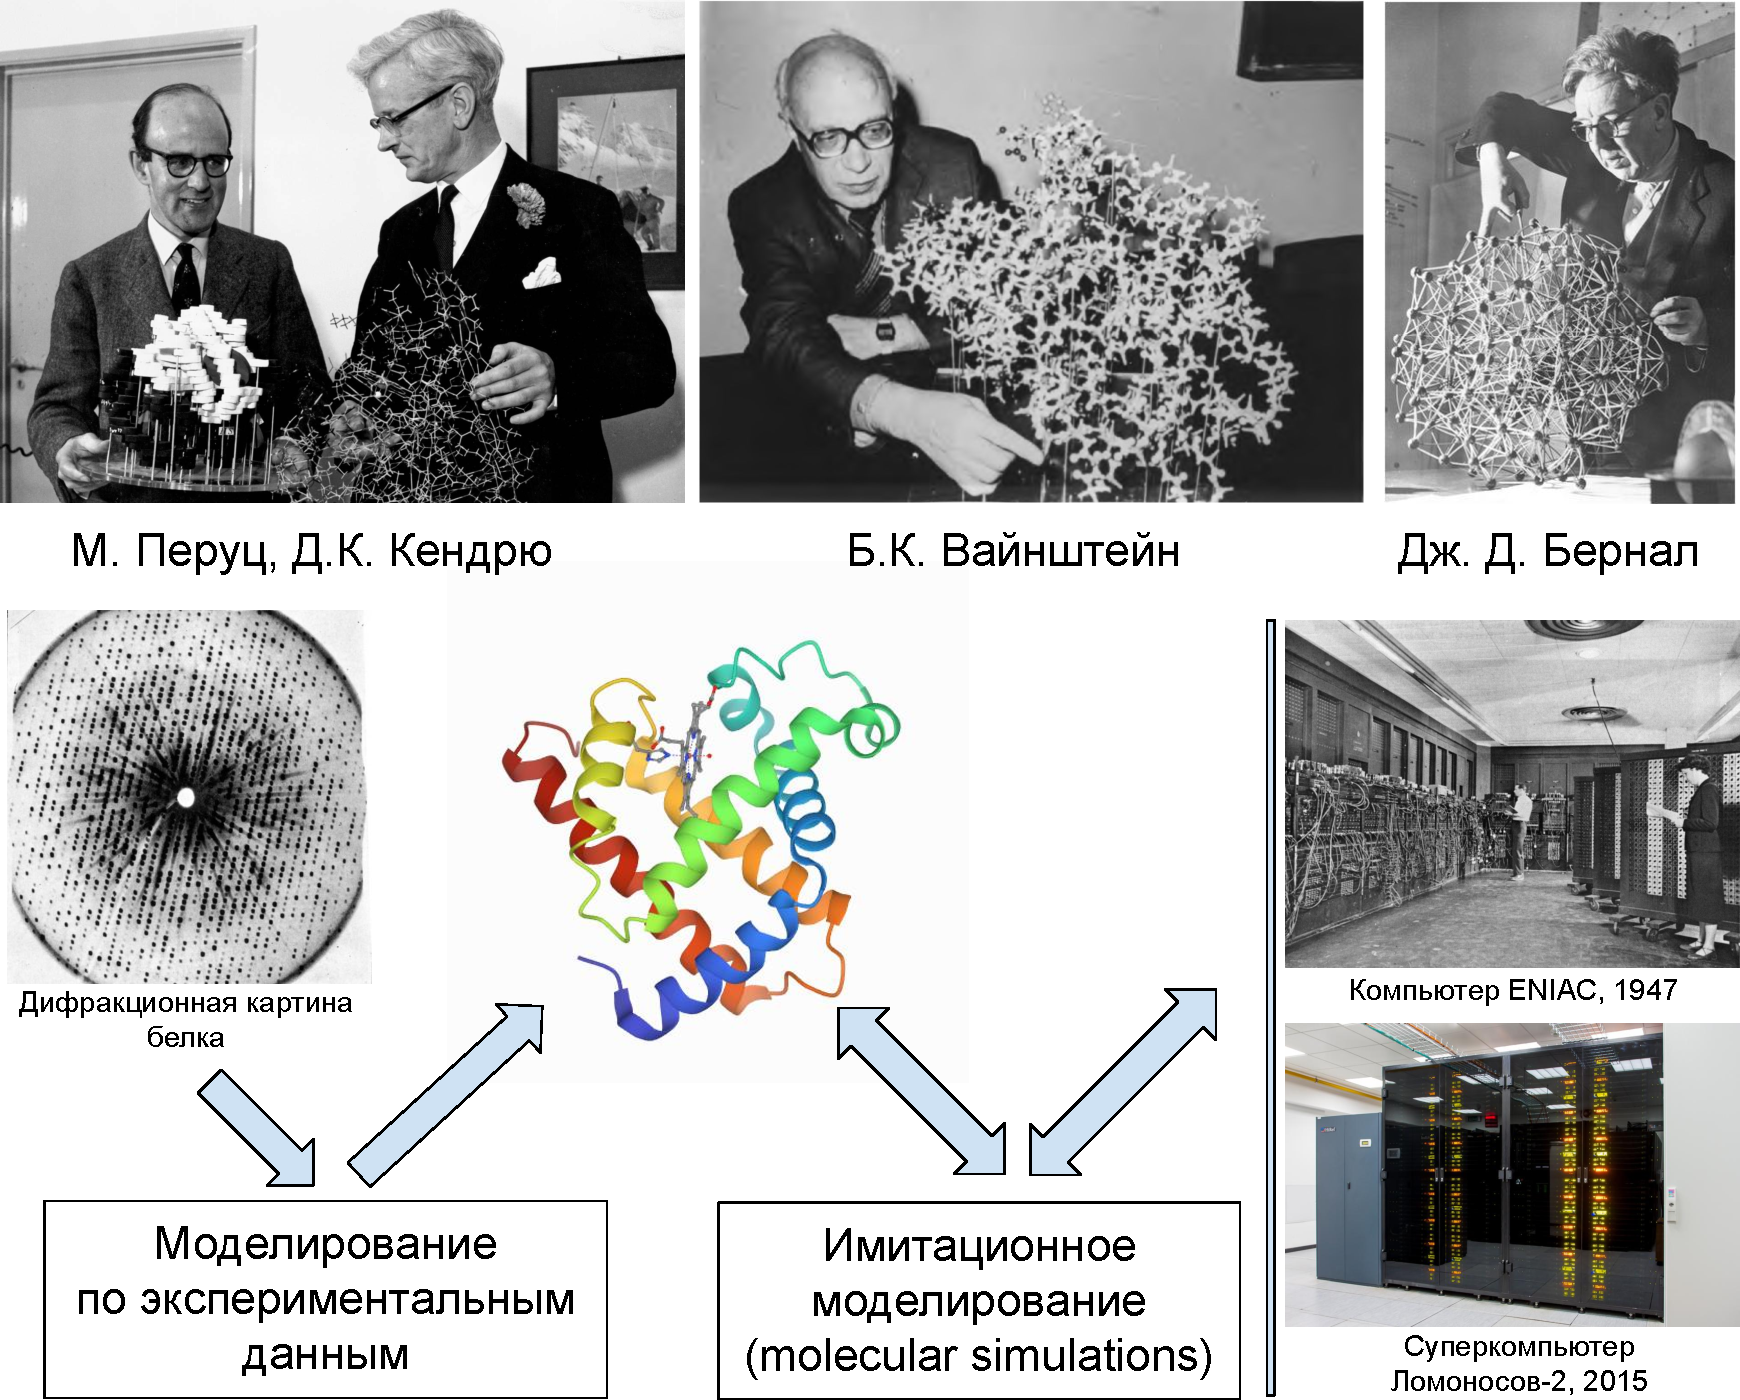
\includegraphics[height=0.85\textheight]{Presentation/images/s1} % окружение figure не требуется
% \begin{columns}
% \begin{column}{0.5\textwidth}
%    some text here some text here some text here some text here some text here
% \end{column}
% \begin{column}{0.5\textwidth}  %%<--- here
%     \begin{center}
%     \begin{itemize}
%         \item Проблема 1 \footnotemark
%         \item Проблема 2
%         \item Проблема 3
%     \end{itemize}
%      \end{center}
% \end{column}
% \end{columns}
% \footnotetext[1]{afjalfjkas}
\note{Изложение сутевой части работы начну с принципиального обсуждения методов и подходов моделирования биомакромолекул. Молекулярное моделирование является одними из важных способов изучения и познания живых систем. На слайде изображен ряд основоположников структурной биологии с физичкскими моделями молекул в руках в эпоху, когда персональные компьютеры еще не были распространены. Уже тогда было понятно, что методы моделирования могут быть подразделены на две группы. В одном случае задача сводится к построению пространственной модели расположения атомов, удовлетворящей наблюдаемым экспериментальным данным (например, ренгеновской дифракции). В другом случае, называемом имитационным моделированием, расположение атомов рассчитывается на основе вычисления внутри- и межмолекулярных взаимодействий между атомами. Развитие компьютеров активно способствовало разработке таких подходов, которые
позволяют рассмотривать в том числе и динамику биомолекул. (1.5-5)

}

\end{frame}


\begin{frame}
\frametitle{Методы молекулярной механики и динамики}
\underline{Полноатомное приближение}
  \begin{small}
   $$ U(\{\vec{r}_i\})= \sum_{bond,ang} \frac{1}{2} k (x-x_0)^2  + \sum_{tors} \frac{1}{2} V_n [1+\cos({n\varphi-\varphi_0})] + \sum_{i,j}^{N} \Bigg\{ 4\epsilon_{ij} \Bigg[\Big(\frac{\sigma_{ij}}{r_{ij}}\Big)^{12} - \Big(\frac{\sigma_{ij}}{r_{ij}}\Big)^6\Bigg] + \frac{q_iq_j}{4\pi \epsilon_0 r_{ij}} \Bigg\} f_{ij} $$
   \end{small}%}

\begin{columns}
\begin{column}{0.45\textwidth}

%\scalebox{0.5}{%

   
     %\label{eq:p1_1:e1}
%\end{multline}}
   \centering
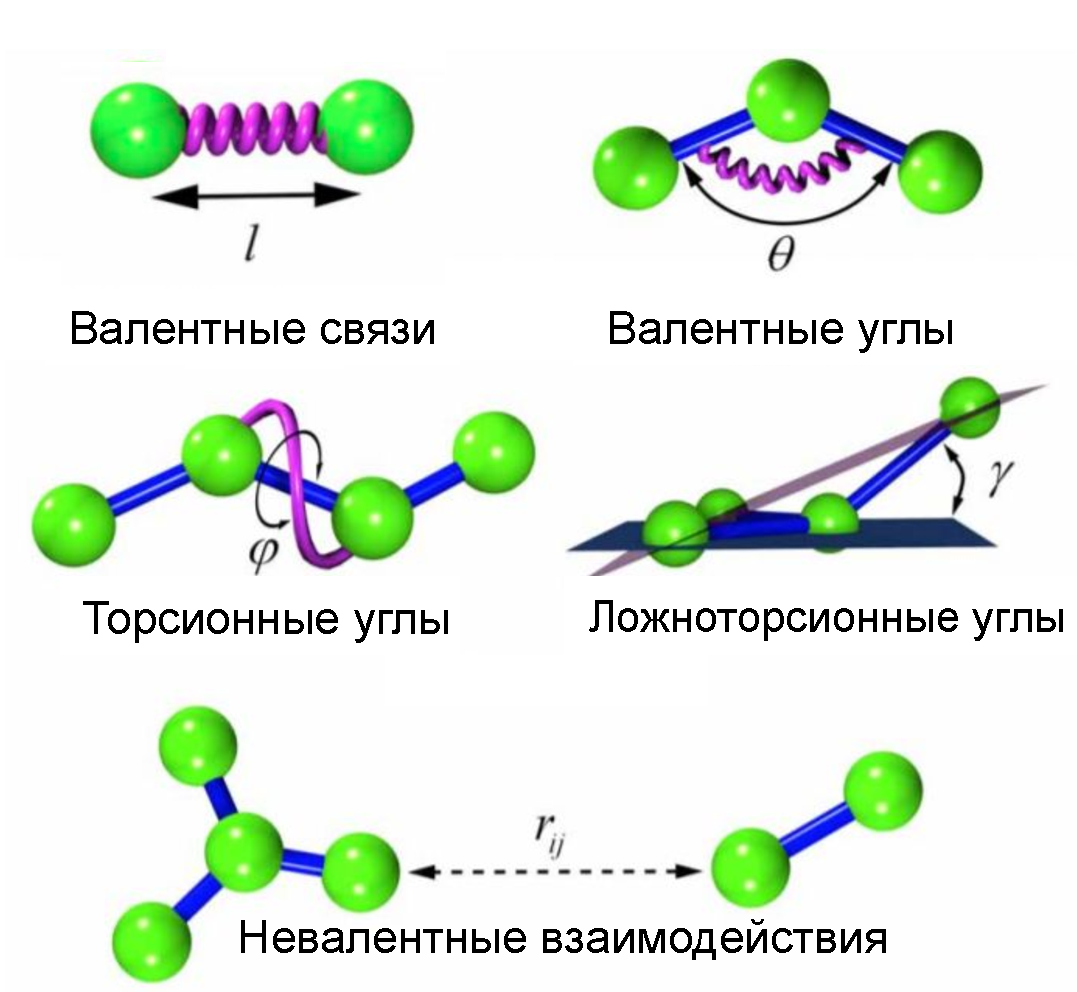
\includegraphics[width=0.8\textwidth]{s2l}
\end{column}
\begin{column}{0.45\textwidth}  %%<--- here
Численное решение уравнений движения ($\vec{F}=m\vec{a}$)
\ifdefined\HANDOUT
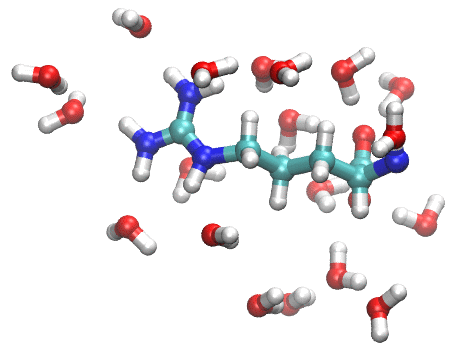
\includegraphics[width=0.8\linewidth]{arg/arg-50}
\else
\animategraphics[autoplay,loop,palindrome,width=0.9\linewidth]{10}{arg/arg-}{0}{50}
\fi
\end{column}
\end{columns}
\note{К таким методам при изучении биообъектов прежде всего относится метод молекулярной динамики. В методе МД физическая модель молекулы представляется в виде набора точечных атомов, взаимодействующим по законам классической механики Ньютона. Функция потенциальной энергии системы обычно задается аддитивным образом на основе комбинации элементарных функций и параметров, называемых силовым полем. В число элементарных взаимодействий входят зарядовые взаимодействия по закону Кулона, дисперсионные взаимодействия на основе потенциала Ван-дер-Ваальса, а также потенциалы, описывающие взаимодействия атомов, связанных химическими связями. Численное решение уравнений движения проводят с применением высокопроизводительного компьютерного и суперкомпьютерного оборудования. Современные вычислительные мощности позволяют достигать микросекундных, а иногда и миллисекундных времен моделирования. На таких временах проявляются термодинамические и статистические свойства молекулярных систем, появляется возможность исследовать различные функциональные процессы. (1.5-6.5)
}
\end{frame}


\begin{frame}
\frametitle{Методы молекулярной механики и динамики}
\underline{Огрубленное приближение} (пример ДНК)
  \begin{small}
   $$     F_k(\{\theta^k_j\})=F_0+\frac{1}{2}\sum_{i=1}^{6}\sum_{j=1}^{6}f_{ij}\Delta\theta^k_{i}\Delta\theta^k_{j}, \; \Delta\theta^k_{i}=(\theta^k_{i}-\hat{\theta}^k_{i}) $$
   \end{small}%}
\begin{columns}
\begin{column}{0.5\textwidth}

%\scalebox{0.5}{%

   
     %\label{eq:p1_1:e1}
%\end{multline}}
   \centering
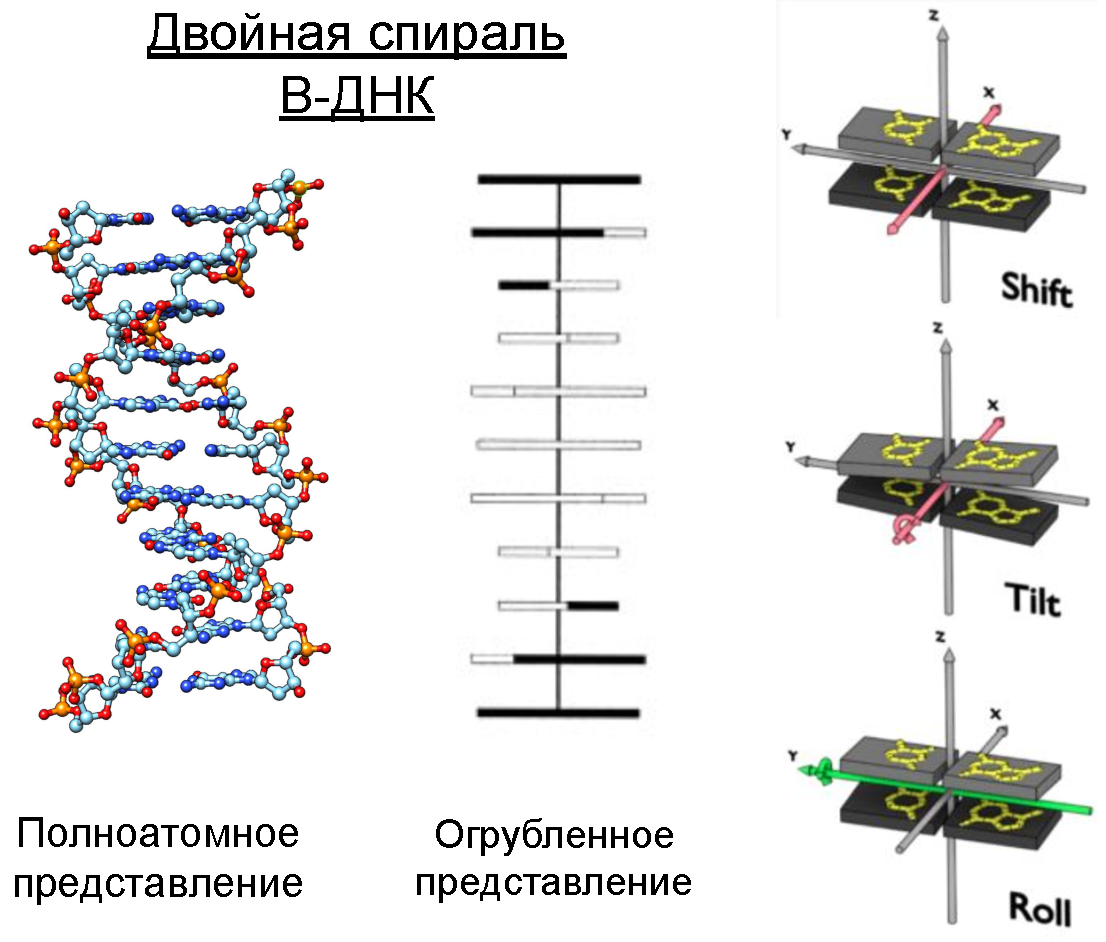
\includegraphics[width=0.7\textwidth]{s3l}
\end{column}
\begin{column}{0.5\textwidth}  %%<--- here
Применение метода Монте-Карло
\begin{center}
\ifdefined\HANDOUT

\includegraphics[width=0.8\linewidth]{DNA/DNAc-100}
\else
\animategraphics[autoplay,loop,palindrome,width=0.6\linewidth]{10}{DNA/DNAc-}{12}{125}
\fi
\end{center}
\end{column}
\end{columns}
\note{\footnotesize{
Свою нишу занимают и так называемые огрубленные подходы к моделированию. В этом случае целая группа атомов может быть представлена в виде некоторой механической единицы. Например, в случае ДНК пара оснований может быть представлена в виде прямоугольника, а функция потенциальной энергии задана как зависимость от взаимного расположения пар оснований. Такие упрощенные модели зачастую позволяют ускорить моделирование, а разумный выбор пространственных координат использовать более гибкие и эффективные подходы к моделированию, например, метод Монте-Карло. (1-7.5)}

}
\end{frame}


\begin{frame}
\frametitle{Проблемы моделирования биомакромолекулярных комплексов}
   {\Large Большой размер $\Longleftrightarrow$ Структурный полиморфизм}
\bigskip
    % \begin{enumerate}
        % \item один
        % \item два
        % \item три
    % \end{enumerate}
\begin{columns}[t]
\begin{column}{0.45\textwidth}
\underline{Экспериментальные ограничения}
 \begin{itemize}
        \item Сложность кристаллизации (РСА)
        \item Сложность деконволюции усредненного сигнала от набора конформаций
        \item Сложность детекции и обработки сигнала (ЯМР)
        \item Неустойчивость комплексов
    \end{itemize}
\end{column}
\begin{column}{0.55\textwidth}  %%<--- here
\underline{Вычислительные ограничения}
 \begin{itemize}
        \item Ограниченные времена моделирования
        \item Времена функциональной динамики комплексов существенно больше
        \item Ограниченная точность силовых полей
        \item Чувствительность конформаций комплексов к точности параметров моделирования
    \end{itemize}
\end{column}
\end{columns}

\note{\footnotesize{Несмотря на существенный прогресс как методов структурной биологии, так и методов вычислительной биофизики, в понимании структурно-динамической организации биомакромолекул имеется ряд затруднений. В особенности это относится к биомакромолекулярным комплексам.

Основных факторов, затрудняющих исследование структурной организации биомолекул, два -- это большой размер и динамический полиморфизм. При этом они взаимосвязаны - большие комплексы зачастую обладают богатым набором конформационных состояний, а отдельные домены могут относится к классу неупорядоченных белков.
В качестве яркого примера можно привести проблему описания упаковки ДНК в ядре эукариотических клеток, которая требует развития новых концептуальных походов на стыке полимерной физики и сруктурной биологии.

Размер и полиморфизм биомакромолекулярных комплексов перпятствует их эффективному изучению классическими методами структурной биологии (рентгеностурктурный анализ, ЯМР, крио-ЭМ).

Однако и моделирование их методами молекулярной динамики также затруднительно.
Осоновных проблемы здесь две. Во-первых, с ростом сложности молекулярной системы увеличиваются и времена функциональной динамики. Например, фолдинг белков проиходит обычно на субмиллисекундных и миллисекундных масштабах, а сборка ДНК-белкового комплекса нуклеосомы занимает уже десятки секунд. Расчеты необходимой длины не всегда достижимы при современном уровне развития вычислительной техники.
Вторая проблемя связана со сложностью задания силовых полей с нужной точностью. Небольшие неточности при задании атом-атомных потенциалов влияют сразу на большое количество взаимодействующих атомов и могут приводить к серьезным отклонениям в поведения системы.(2-9.5)

}}
\end{frame}

% \begin{frame}
% \frametitle{Виды экспериментальных данных о структуре и динамике биомолекул}

% \note{РСА, ЯМР,}
% \end{frame}

\subsection{Интегративные подходы}

\begin{frame}
\frametitle{Интегративные подходы}
   \centering
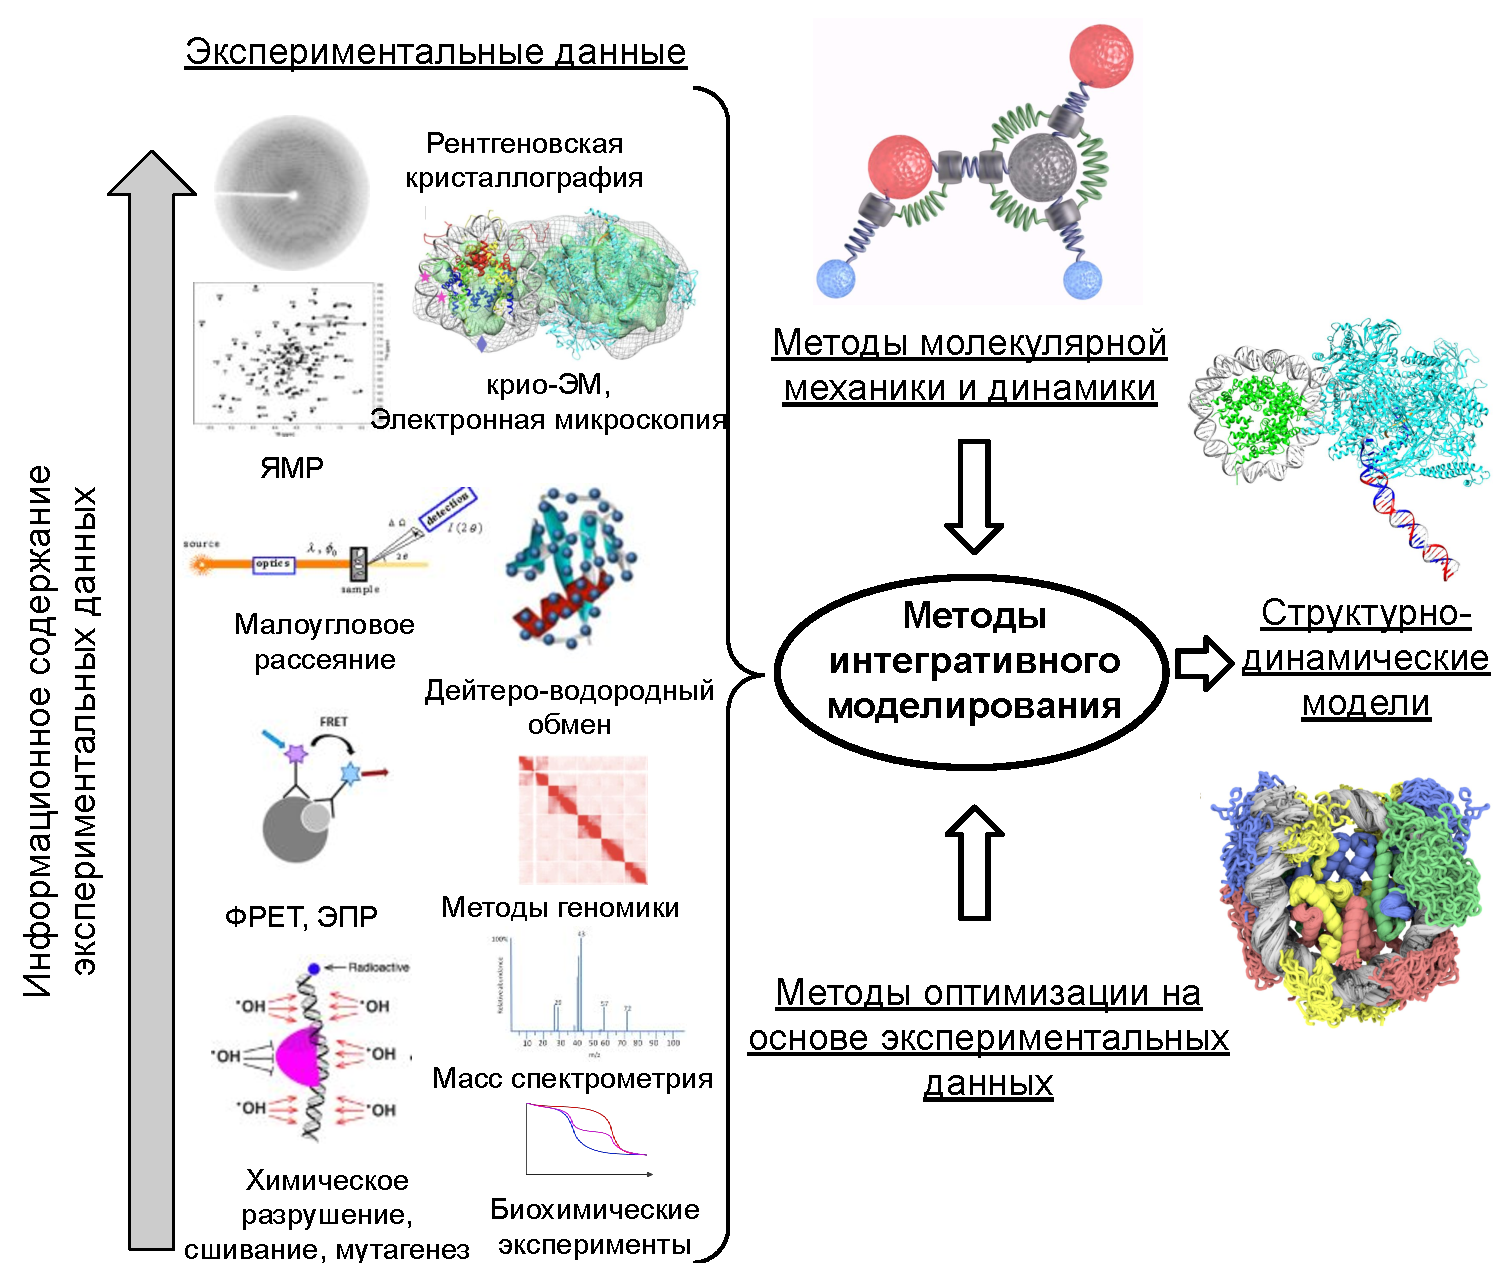
\includegraphics[height=0.9\textheight]{images/p1/int_mod.pdf}
\note{
\footnotesize{Для преодоления вышеозвученных проблем перспективным является развитие интегративных подходов к моделированию биомолекул и их комплексов.
Такие подходы предполагают интеграцию различных экспериментальных данных при построении структурно-динамических моделей биомолекул. В вычислительном плане могут применяться как возможности оптимизационного моделирования, так и имитационного моделирования на основе расчета взаимодействий между атомами.
При применении метода молекулярной динамики стандартной практикой явяляется использование экспериментально определенной стартовой конформации комплекса методами РСА, крио-ЭМ.
Для многих биологических комплексов, однако, экспериментально определенные струкутры либо отсутвуют вообще, либо неизвестны представляющие функциональные интерес конформации. В то же время часто имеются различные экспериментальные данные косвенной природы, получаемые в ходе биофизических, биохимических, функциональных, спектроскопических и других экспериментов. Такого рода эксперименты могут предоставлять информацию о расстояниях между введенными метками в белке или ДНК (например, методы FRET, ЭПР), характере укладки белковой цепи (например, ИК-, КД-спектроскопия, дифракция рентгеновских лучей на фибриллах),
реакционной доступности химических групп (методы футпринтинга, химического сшивания) и др. Задача интегративных подоходов состоит в использовании и такого рода информации.
Далее в диссертационной работе на ряде примеров будет продемонстрировано, каким образом это можно сделать. (2-11.5)}}
\end{frame}



\section[Глава 2]{Глава 2. Применение методов молекулярной динамики для изучения нуклеосом.}

\begin{frame}
\frametitle{Проблема понимания структуры хроматина}
\centering
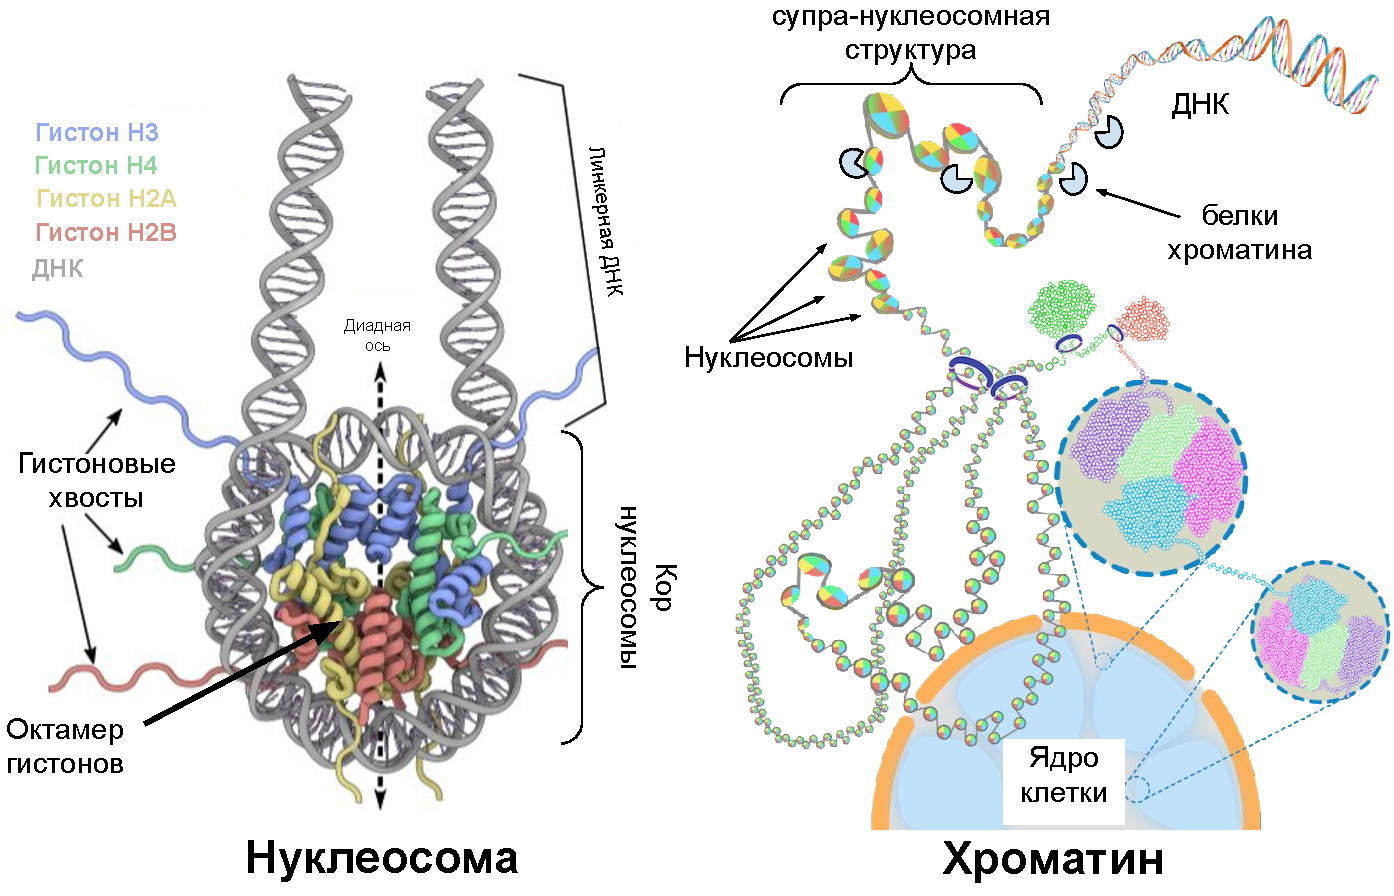
\includegraphics[width=1.0\textwidth]{s9}
\note{Первая часть работы посвящена исследованию струкутрно-динамической организации нуклеосом и их комплексов с белками хроматина. Хроматин - это набор ДНК, РНК и белков, находящихся в ядре эукариотических клеток. Нуклеосомы являются базовыми элементарными единицами хроматина. Они состоят из примерно 200 пар оснований ДНК, организованных гистоновыми белками. Центральные 147 пар оснований ДНК образуют коровую частицу нуклеосомы, плотно наматываясь на октамер гистонов в виде полутора витков левой суперспирали. Нуклеосомы претерпевают множество важных структурных и динамических перестроек во время всех ключевых процессов транскрипции, репликации, репарации ДНК и т.д. Способность нуклеосом претерпевать определенные типы конформационных переходов играет важную роль при взаимодействии с белками, включая ремоделирующие комплексы, факторы транскрипции, шапероны, РНК-полимеразы и т.д. (1.5-13)
}

\end{frame}

\begin{frame}
\frametitle{Проблема динамики нуклеосом}

\centering
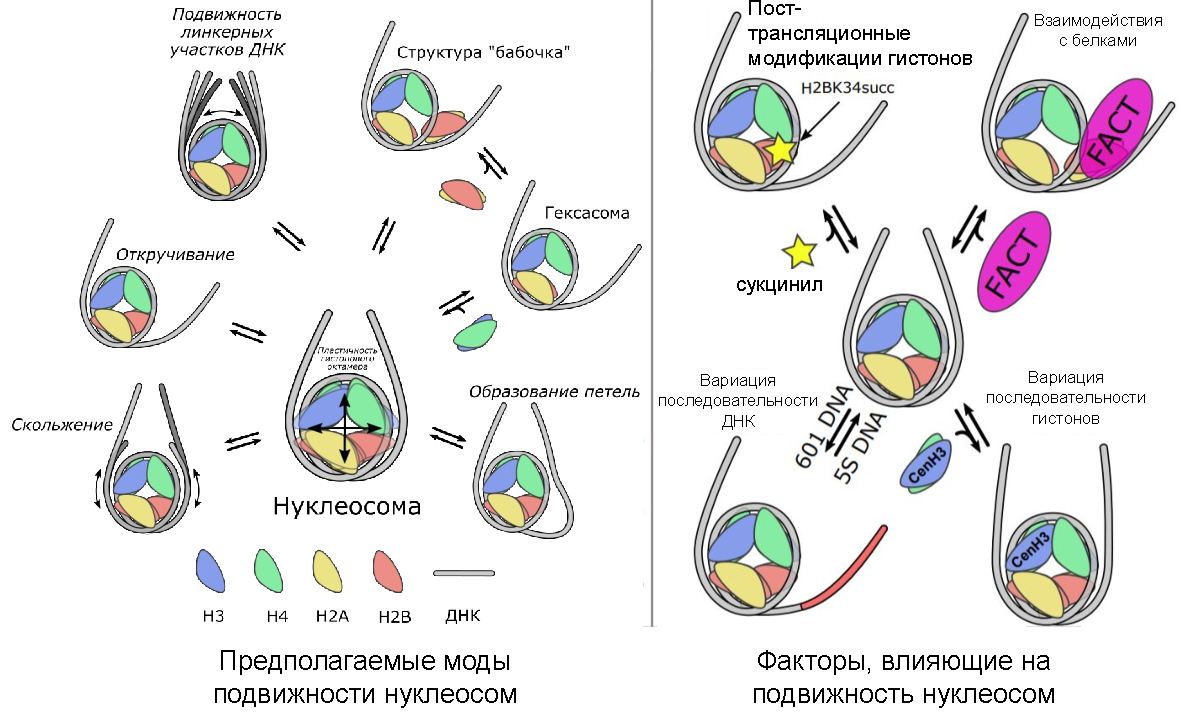
\includegraphics[width=1.0\textwidth]{s10}

\note{На слайде проиллюстрированы предполагаемые динамические режимы нуклеосом и влияние на них различных факторов:
последовательности ДНК и гистонов, пост-трансляционных модификаций аминокислот гистонов, взаимодействия с белками. Динамика нуклеосом может происходить спонтанно при данной температуре или носить функционально направленный характер за счет воздействия специальных АТФ-зависимых комплексов. Белковый состав и последовательность ДНК в нуклеосомах влияют на характер динамических процессов в нуклеосомах и таким образом модулируют различные функциональные процессы в геноме. Так показано существование тонких режимов конформационной динамики нуклеосом. Например, кручение ДНК внутри нуклеосомы обеспечивает путь для АТФ-зависимого передвижения нуклеосом вдоль ДНК. Речь идет о существовании особых режимов динамики нуклеосом, в которых важны атомостические детали структурных изменений.

В то же время, методами структурной биологии с высоким разрешением хорошо изучена лишь одна компактная конформация коровой частицы нуклеосомы, которую удалось закристаллизовать.

 Метод молекулярной динамики является мощным инструментом, который может раскрыть природу различных динамических состояний нуклеосом на атомистическом уровне. (1.5-14.5)
	
}
\end{frame}


\begin{frame}
\frametitle{Полноатомные расчеты нуклеосом методом МД}
Расчет нуклеосомы с линкерной ДНК на масштабе 1 мкс
\begin{columns}[b]
\begin{column}{0.37\textwidth}
\begin{center}
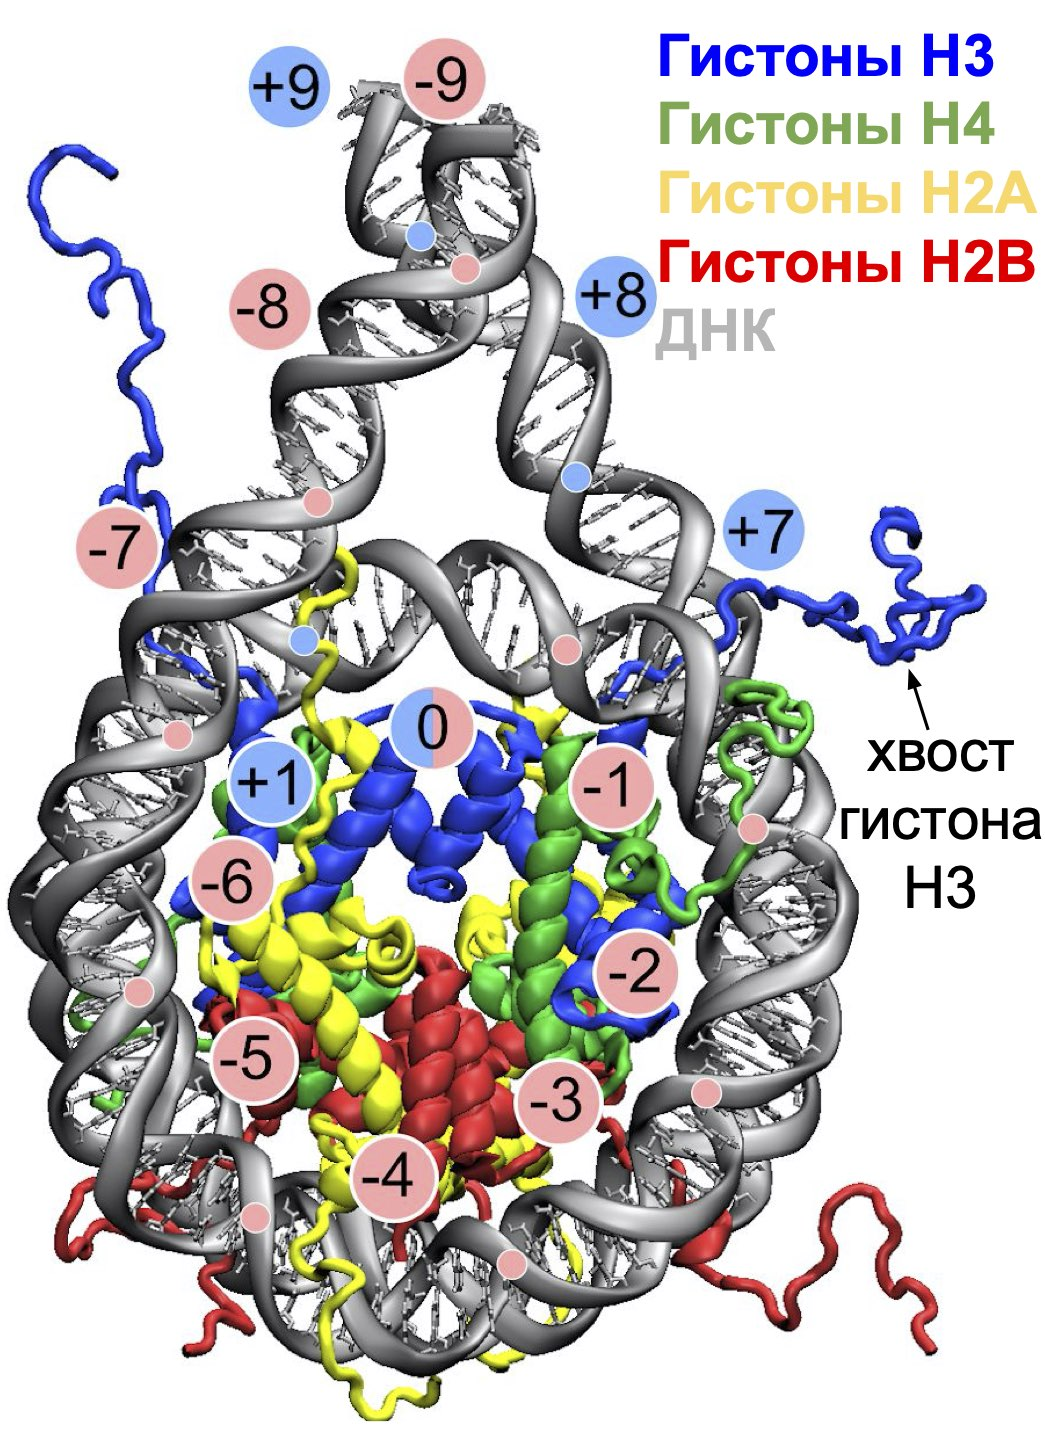
\includegraphics[width=1.0\textwidth]{s11l.jpg}
\textbf{t=0 мкс}
\end{center}
\end{column}
\begin{column}{0.32\textwidth}  %%<--- here
\begin{center}
\ifdefined\HANDOUT
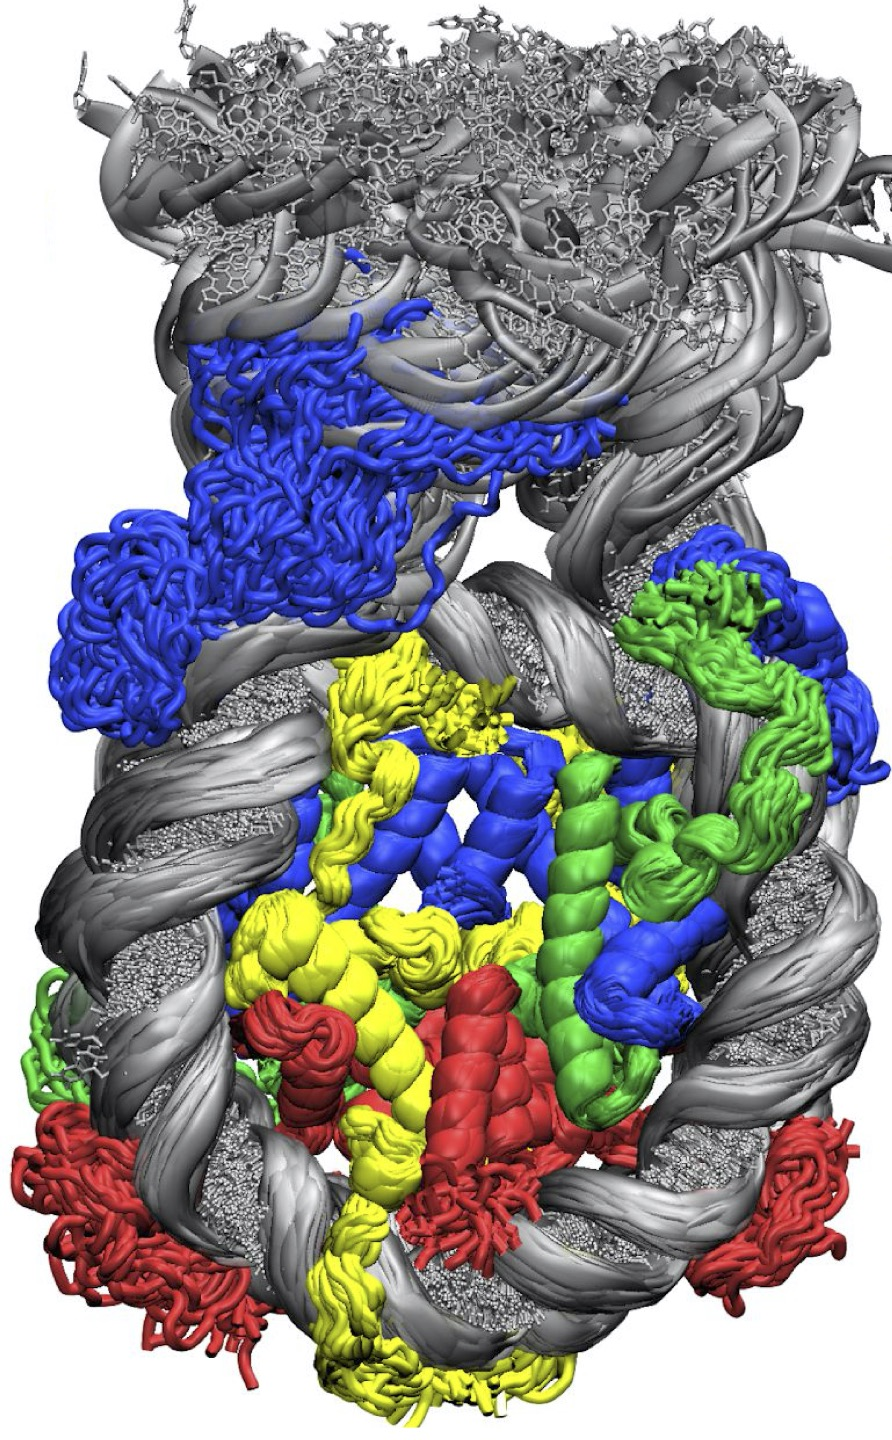
\includegraphics[width=1.0\linewidth]{1mus/1mus1}
\else
\animategraphics[width=1.0\linewidth]{10}{1mus/1mus}{1}{100}
\fi
%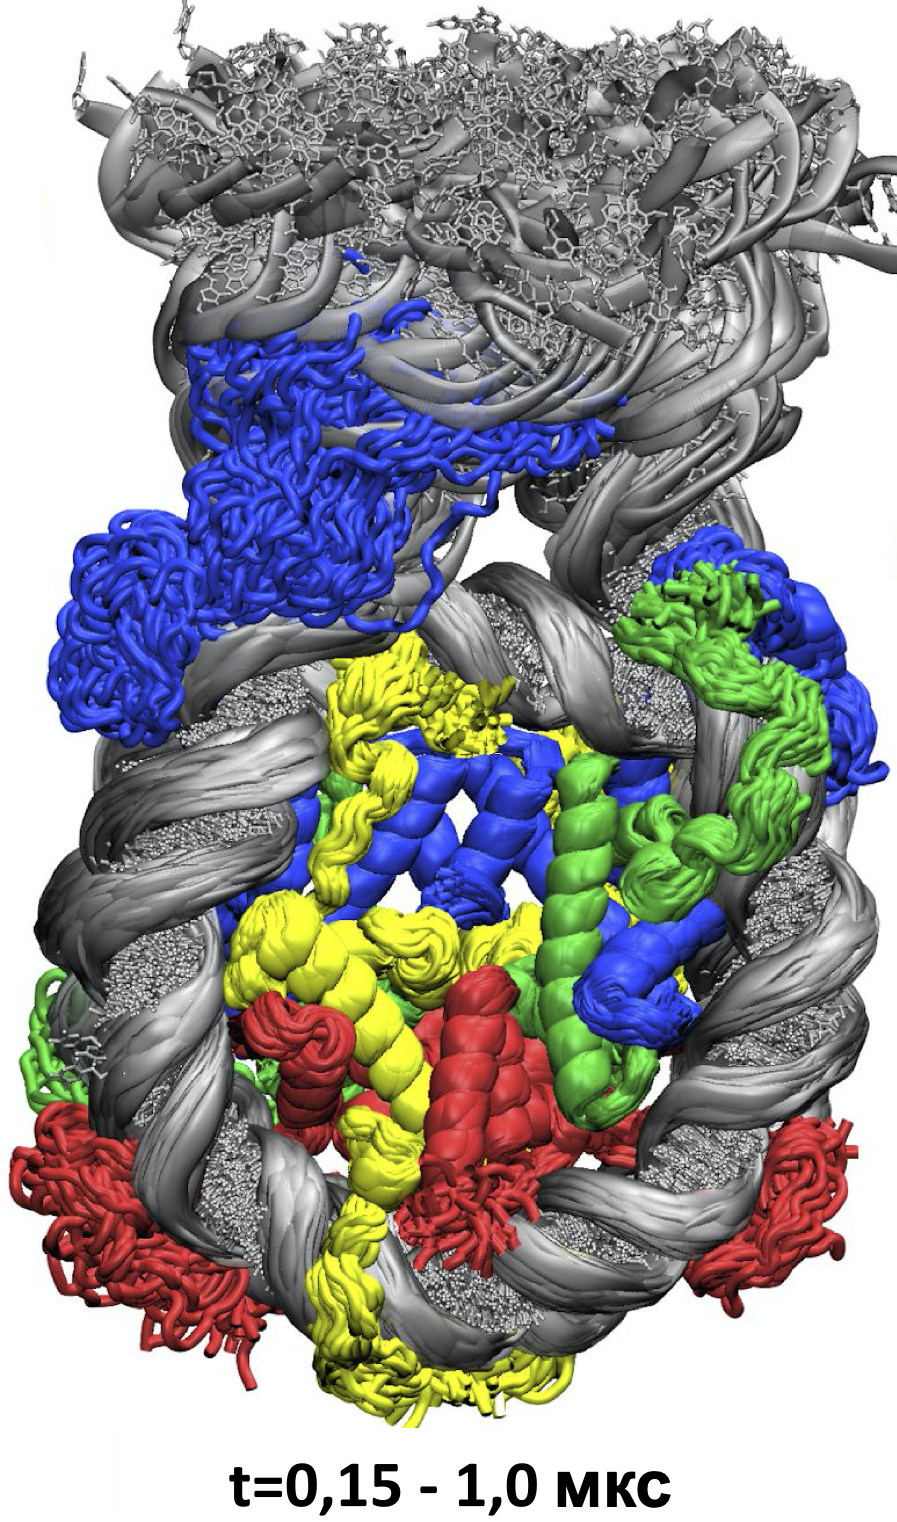
\includegraphics[width=1.0\textwidth]{s11m}
\textbf{t=0,15-1 мкс}
\end{center}
\end{column}
\begin{column}{0.31\textwidth}  %%<--- here
\begin{center}
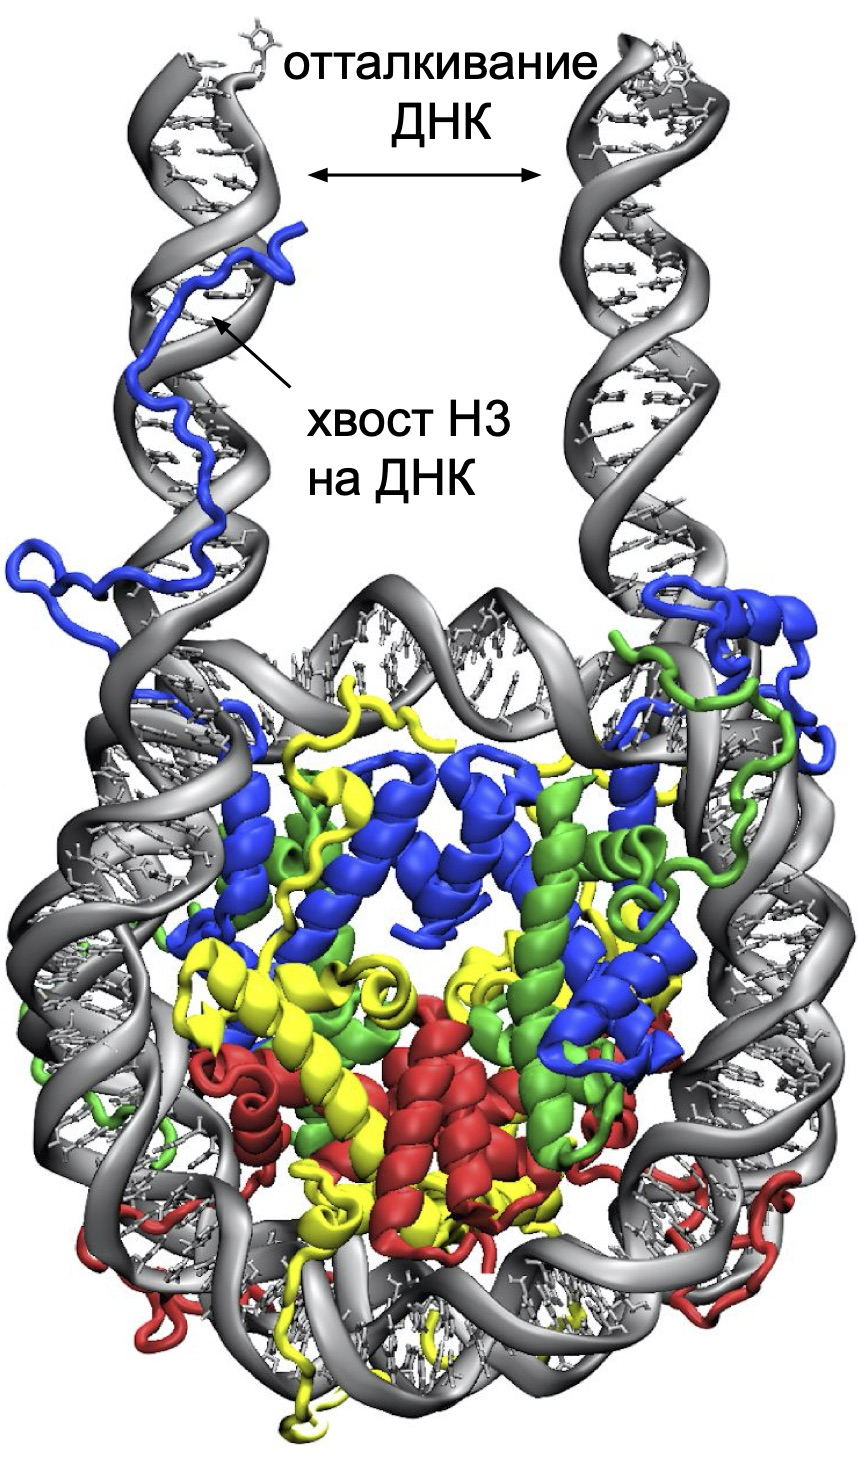
\includegraphics[width=1.0\textwidth]{s11r.jpg}
\textbf{t=1 мкс}
\end{center}
\end{column}
\end{columns}


%\centering
%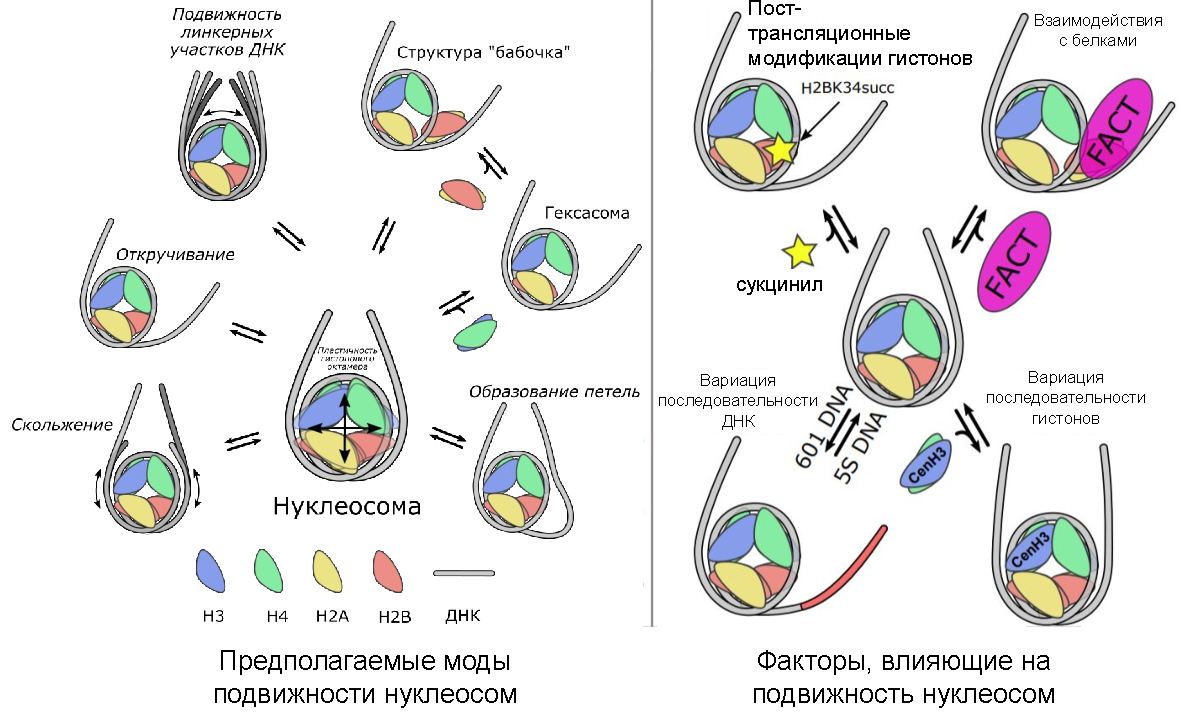
\includegraphics[width=1.0\textwidth]{s10}
% \includemedia[
%   %activate=onclick,
%   addresource=videos/nucl1mus.mp4,
%   flashvars={
%      source=videos/nucl1mus.mp4
%     &autoPlay=true
%     &loop=true
% },
%   passcontext
% ]{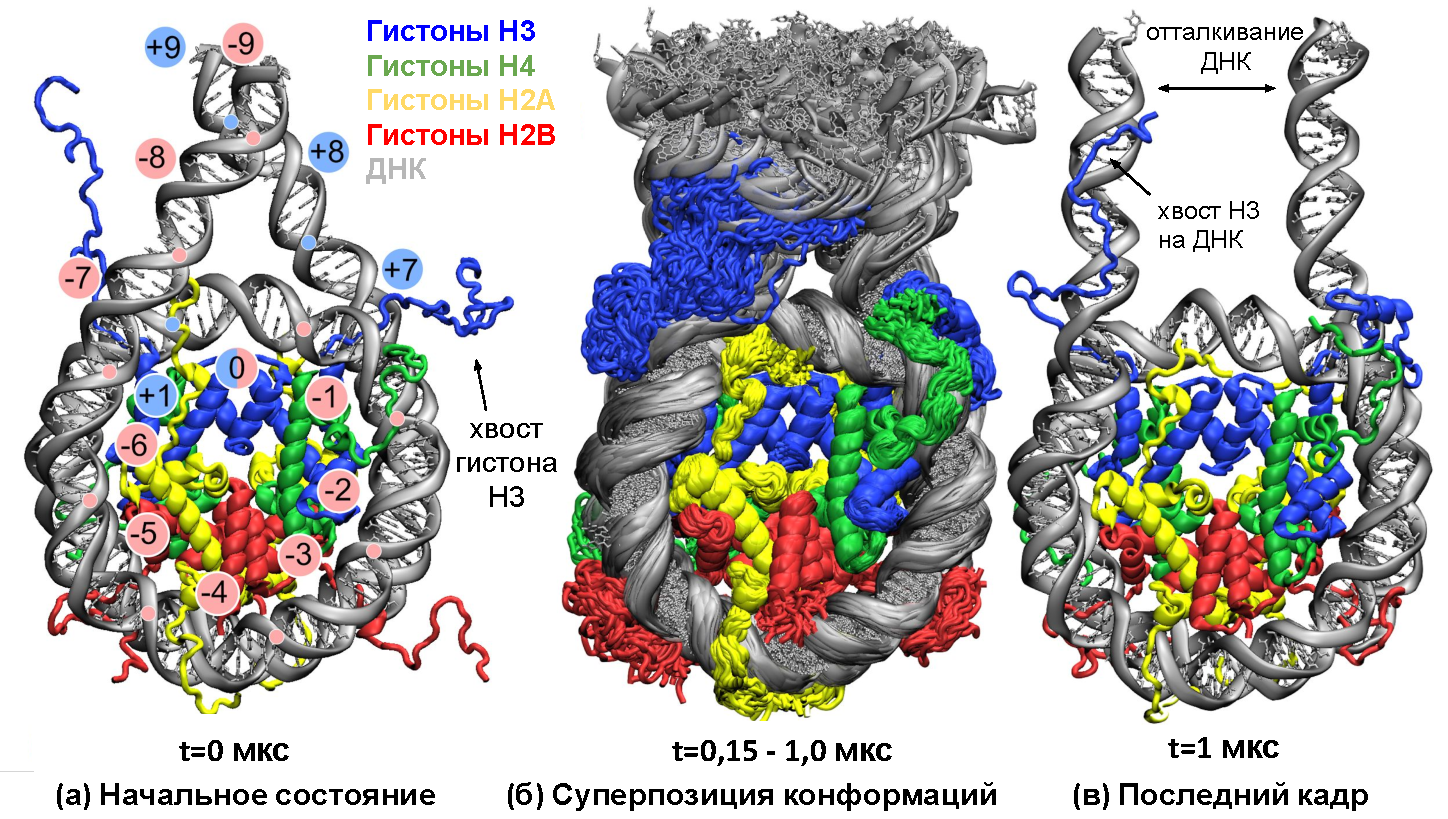
\includegraphics[height=0.45\linewidth]{images/p2/jmb/part2_2_f1}}{VPlayer9.swf}

\note{
	\tiny{Нами были разработаны подходы и алгоритмы моделирования нуклеосом методами молекулярной динамки в полноатомном приближении в явном растворителе на микросекундном и мульти-микросекундном временном диапазоне с использованием суперкомпьютерных технологий.  Также разработаны алгоритмы анализа траекторий, в частности задания нуклеосомной системы координат на основе определения оси суперспирали ДНК и оси псевдосимметрии нуклеосомы. В результате стало возможным определение различных геометрических параметров молекулярной системы таких, как геометрия ДНК, углы вращения ДНК, расположение остова полипептидных цепей. На данном слайде приводятся результаты равновесного микросекундного моделирования молекулярной динамики нуклеосом, включающих линкерные сегменты ДНК и полноразмерные гистоны. Выявлено, что линкерные участки ДНК изменяют свое взаимное расположение из-за электростатического отталкивания, что влияет на углы входа-выхода ДНК из нуклеосом и следовательно на структуру супрануклеосомной организации хроматина. Если в начальной структуре гистоновые хвосты экспонированы в растворитель, то в ходе динамики их конденсация на ДНК происходит в течение нескольких десятков наносекунд. Далее начинается диффузия хвостов вдоль поверхности ДНК. При этом хвосты могут принимать конформационно ограниченные позиции из-за вставки лизинов и аргининов в малые бороздки ДНК.
  %Мы показали, что определенные конформации гистонового хвоста способствуют выпячиванию ДНК вблизи участков ее входа/выхода в/из нуклеосомы, что приводит к образованию дефектов кручения внутри ДНК.
  Ряд аминокислот в гистоновых хвостах, являются сайтами важных эпигенетических пост-трансляционных модификаций. Видно, что многие из этих сайтов находятся в тесном контакте с ДНК, что ограничивает их доступность для пост-трансляционной модификации и взаимодействий с белками хроматина. Такие взаимодействия способствуют и возникновению кооперативных эффектов при связывании нескольких белков с соседними сайтами на гистоновых хвостах. Полученные результаты находятся в согласии с экспериментами по химическому сшиванию гистонов с ДНК, ЯМР-анализу.(2.5-17)}}
\end{frame}


\begin{frame}
\frametitle{Мульти-микросекундные МД расчеты нуклеосом}
%\embedvideo{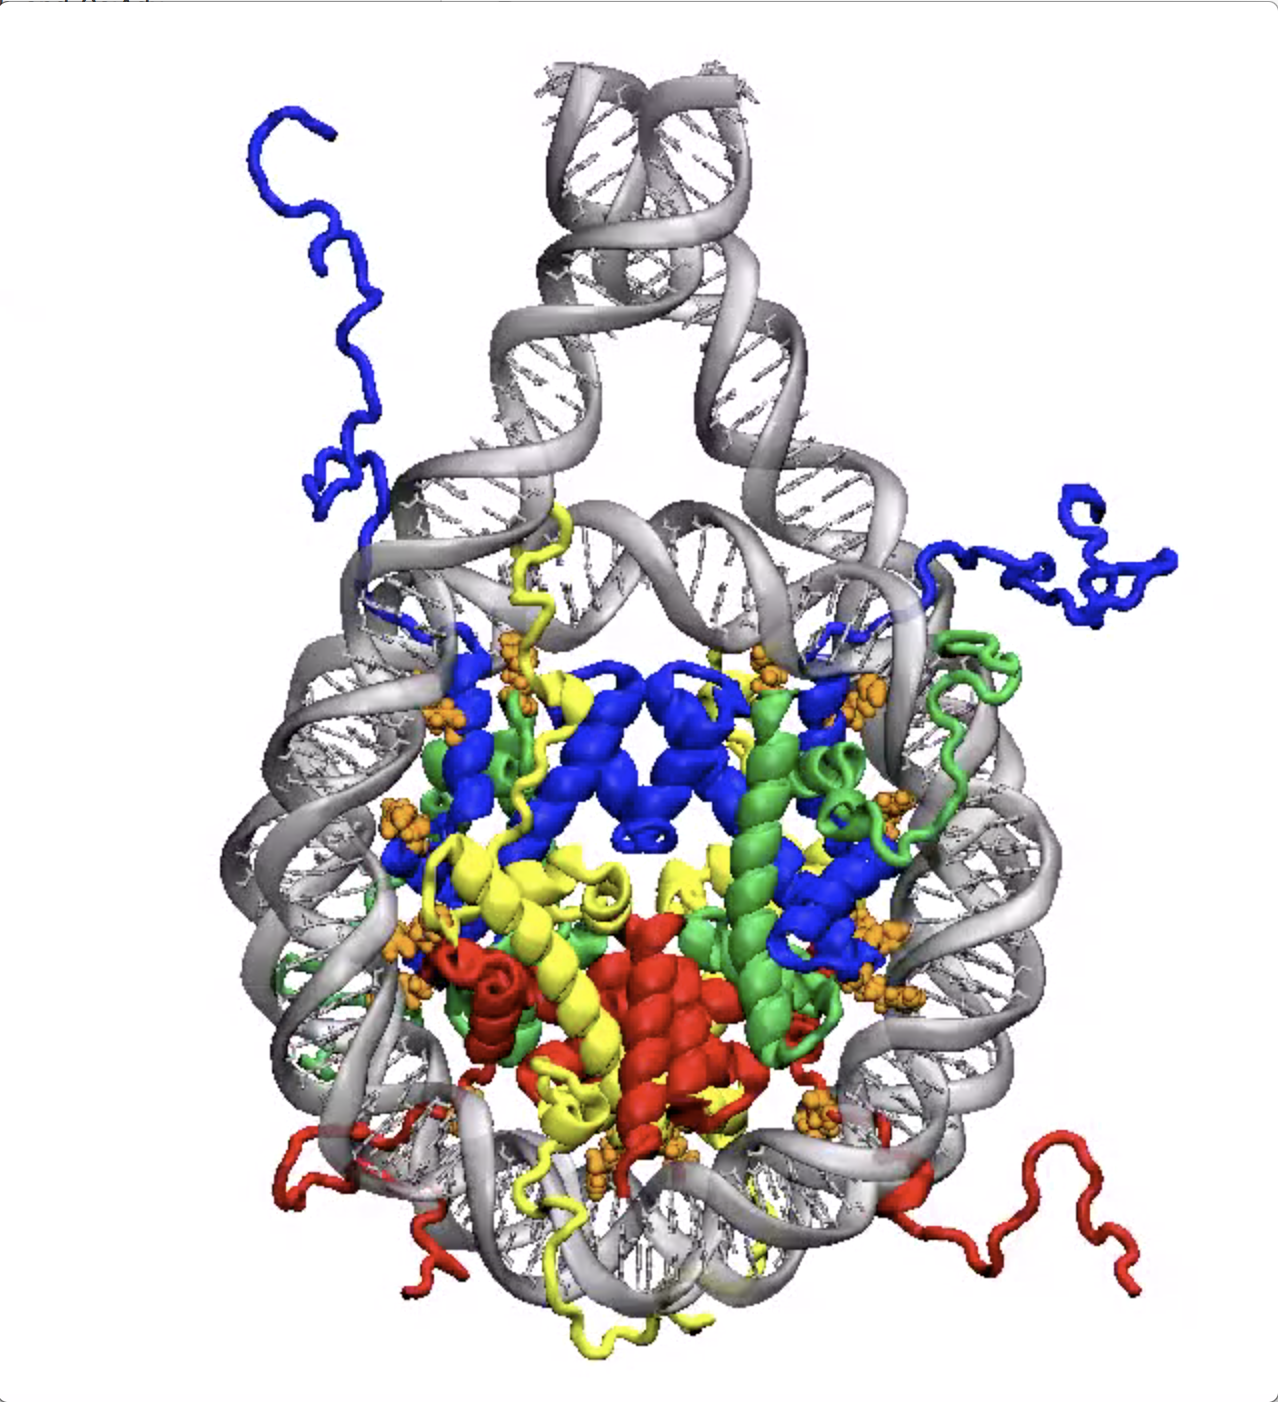
\includegraphics[width=0.45\textwidth]{Presentation/images/nucl1mus}}{videos/nucl1mus.mp4}

Расчет коровой частицы нуклеосомы на масштабе > 10 мкс
\begin{columns}[b]
\begin{column}{0.3\textwidth}
\begin{center}
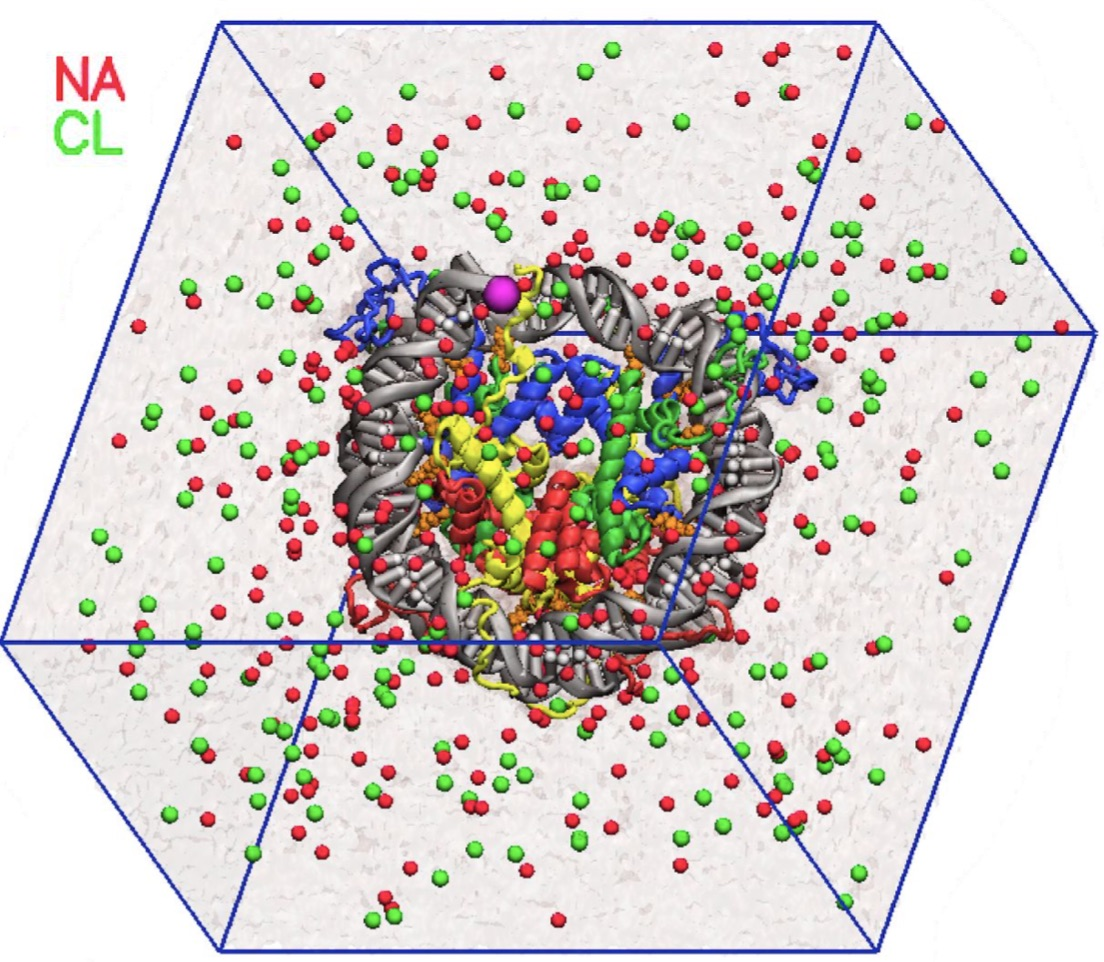
\includegraphics[width=1.0\textwidth]{s12l.jpg}
Расчетная система в растворителе
\end{center}
\end{column}
\begin{column}{0.45\textwidth}  %%<--- here
\begin{center}
% \animategraphics[width=1.0\linewidth]{10}{10mus/10mus}{1}{100}
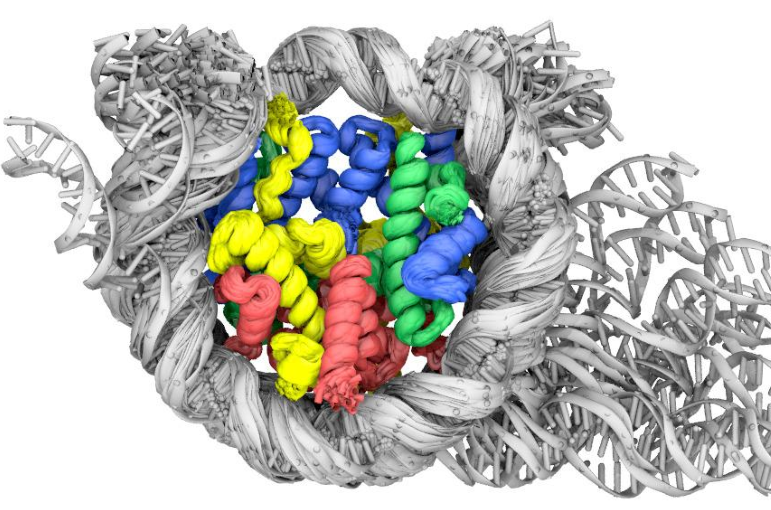
\includegraphics[width=1.0\textwidth]{s12m}
Динамика системы
\end{center}
\end{column}
\begin{column}{0.25\textwidth}  %%<--- here
\begin{center}
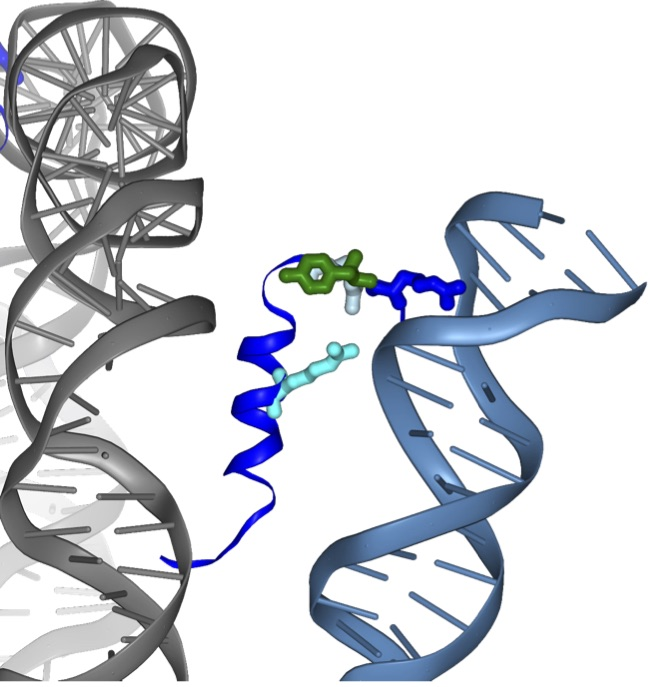
\includegraphics[width=1.0\textwidth]{s12r.jpg}
Динамика гистонов влияет на откручивание ДНК
\end{center}
\end{column}
\end{columns}

\note{\scriptsize{На данном слайде представлено развитие предыдущей работы - моделирование коровых частиц нуклеосом на временах более 10 мкс, которое стало возможным и благодаря прогрессу вычислительных технологий и разработанной нами автоматической системе подготовки, запуска и анализа расчетов. На столь длинных временах мы впервые наблюдали диссоциацию и откручивание ДНК от гистонового октамера. В ходе моделирования были выявлены ключевые взаимодействия ДНК-белок с гистонами, которые являются барьерами для откручивания ДНК от октамера гистонов. На рисунке показана такая область белка вблизи конца нуклеосомной ДНК. Механизм сцепления двух супервитков ДНК заключается в том, что боковые цепи соседних аминокислот взаимодейстуют с малыми бороздками. Потеря одного из контактов приводит к возникновению флуктуаций ДНК. В ходе моделирования также была показана возможность локального спонтанного изменения степени закрученности ДНК (образование/релаксация так называемых дефектов кручения) и сдвиг ориентационного положения для части коровой ДНК. Данные наблюдения указывают на возможность транслокации ДНК вдоль нуклеосомы путем “червячного” передвижения дефектов кручения вдоль ДНК (inchworm meсhanism). При этом ДНК подобно винту прокручивается вдоль поверхности октамера гистонов. В ходе моделирования также было показано наличие динамической пластичности ядра гистонов, способствующей подвижности ДНК. В результате сравнительного моделирования нуклеосом с хвостами и без хвостов гистонов было выявлено, что гистоновые хвосты замедляют как время отворачивания, так и время приворачивания ДНК, а также при отворачивании ДНК удерживают ее вблизи исходной траектории. (2.5-19.5)}}
\end{frame}

\section[Глава 3]{Глава 3. Интегративное моделирование с применением данных экспериментов по футпринтингу ДНК.}


\begin{frame}
\frametitle{Метод гидроксильного футпринтинга}

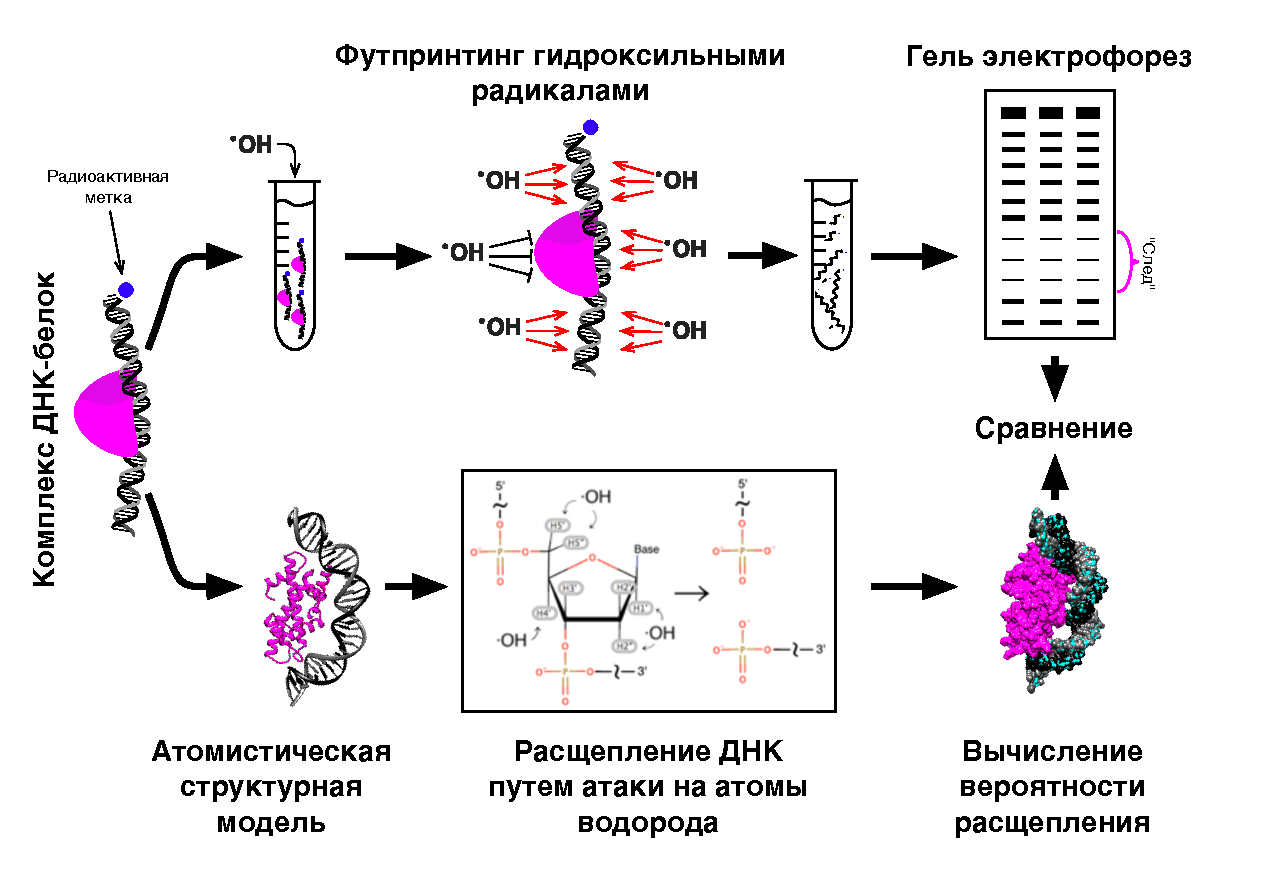
\includegraphics[width=1.0\textwidth]{images/p5/part5_1_np/p5_1_f1.pdf}

\note{Процессы динамики нуклеосом, изученные нами методом МД, ограничены по времени в силу текущих вычислительных возможностей. Крупномасштабные процессы, например, скольжения нуклеосом вдоль ДНК, сборка и разборка нуклеосом, полная диссоциации/реассоциации ДНК пока находятся за пределами моделируемых временных интервалов. Примером задачи не решаемой методами МД является выбор нуклеосомой наиболее энергетически выгодного оптимального положения на большом участке ДНК. Для решения такой задачи могут применяться интегративные подходы. В главе 3 развиты подходы по моделированию ДНК-белковых комплексов, основанные на использовании экспериментальных данных по расщеплению ДНК (футпринтингу) гидроксильными радикалами. Гидроксильные радикалы обладают высокой реакционной способностью, небольшим размером, не являются заряженными. При взаимодействии с ДНК они атакуют атомы водорода дезоксирибозы, что приводит к расщеплению ДНК с потерей атакованного нуклеотида. При наличии белка на ДНК, белок стерически экранирует ДНК от расщепления. Это свойство можно использовать для анализа структуры ДНК-белковых комплексов. Общая схема данного подхода представлена на слайде.(1.5-21)}
\end{frame}


\begin{frame}
\frametitle{Проблема интерпретации данных футпринтинга ДНК}
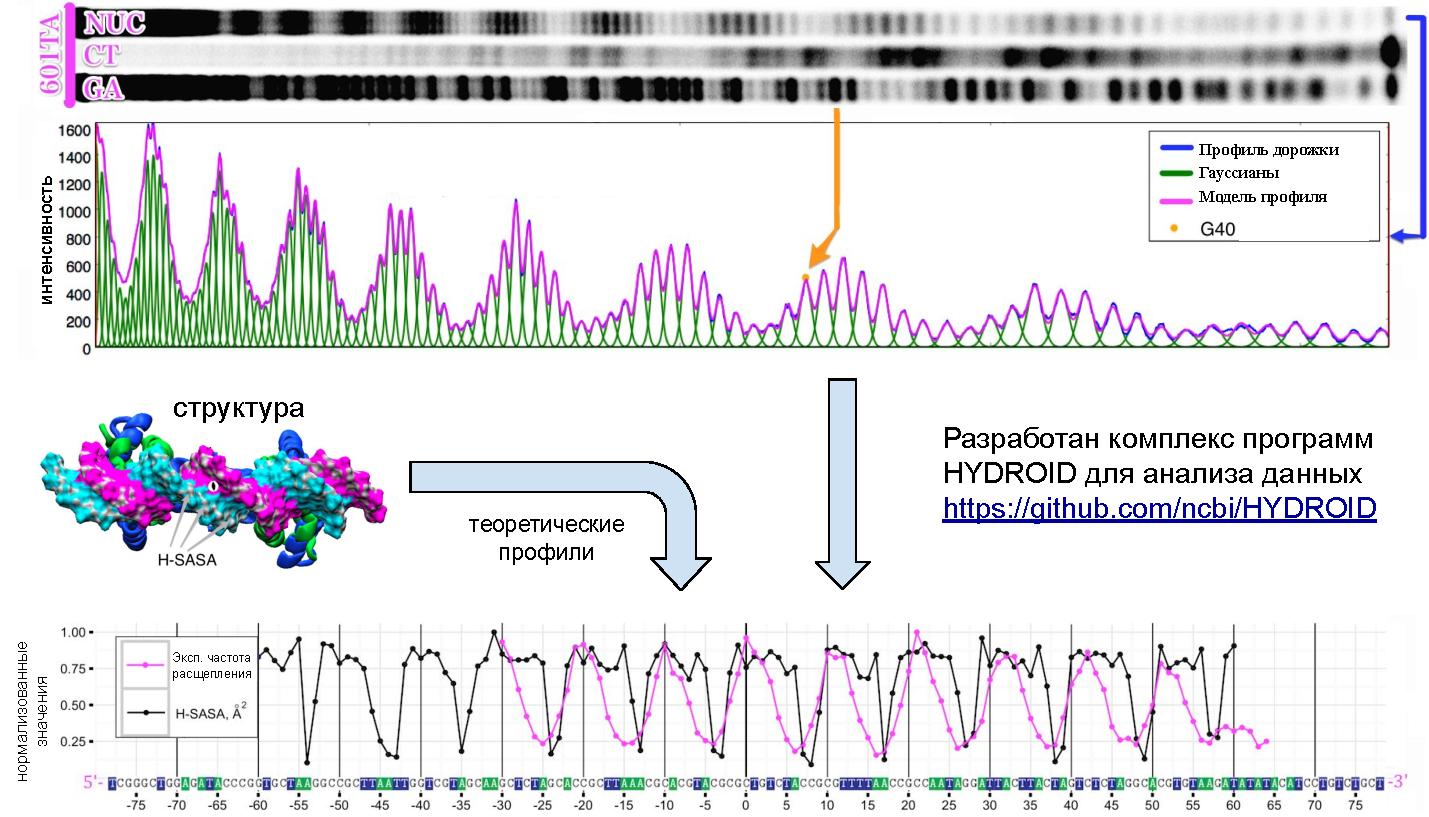
\includegraphics[width=1.0\textwidth]{s14}

\note{В методе гидроксильного футпринтинга фрагменты расщепленных молекул ДНК визуализируют с помощью метода гель-электрофореза. Гель электрофорез разделяет молекулы по длине и формируется характерная картина полос разной интенсивноси. При этом суммарная интенсивность полосы пропорциональна вероятности расщепления ДНК в конкрентной позиции. У каждой полосы присутствует диффузионное размытие, зависящее от длины фрагмента ДНК. Определение интенсивности полос требует аппрокисмации данных в виде математической модели (каждая полоса описывается гауссом). Нами был разработан программный продукт HYDROID позволяющий вычислять профили интенсивонсти расщепления ДНК по изображениям гель электрофореза, а с другой стороны оценивать эту величину на основе моделей ДНК-белковых комплексов. Для оценки был разработан алгоритм, который оценивает доступность атомов водорода деоксирибозы для атаки гидроксильными радикалами.(1.5-22.5)}
\end{frame}


\begin{frame}
\frametitle{Определение позиционирования ДНК на нуклеосоме}
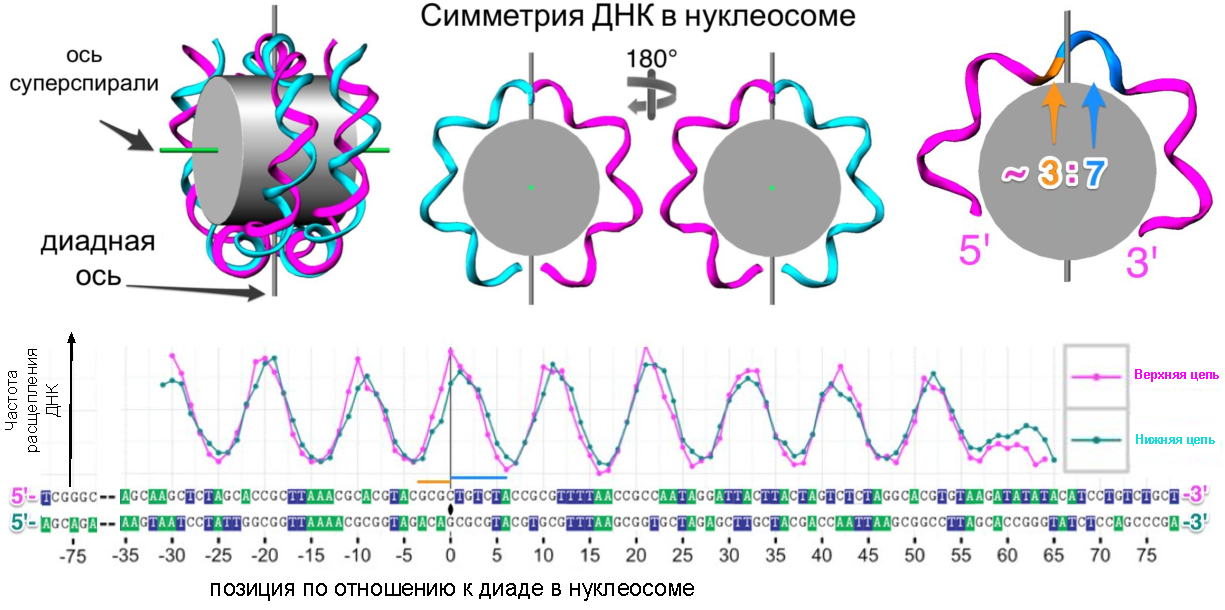
\includegraphics[width=1.0\textwidth]{s15}
\note{Используя разарботанные подоходы по обработке экспериментальных данных гидроксильного футпринтинга, а также теоретического моделирования этого процесса на основе структурных моделей, нами был разработан алгоритм, который позволяют точным образом определить положение ДНК в нуклеосоме. Дело в том, что в зависимости от характеристик ДНК сиквенса стабильность нуклеосомы может отличаться на 2-4 ккал/моль. Таким образом, на длинном фрагменте ДНК белковое ядро соберется в определенной выгодной конфигурации. Оказывается, что определить эту конфигурацию можно по данным футпринтинга с точность до одного нуклеотида, если учесть свойства симметрии нуклеосомы. Поскольку нуклеосома обладает осью псевдо симметрии второго порядка, то при повороте на 180 градусов одна цепь ДНК занимает положение другой. Это проявляется и в совпадении профилей футпринтинга для двух цепей ДНК, если они выровнены по нулеотидоной паре, лежащей на оси симметрии - диаде. А если эта пара не известна, то ее можно установить решив обратную задачу и таким образом опеределить положение ДНК на белковом ядре. (1.5-24)}
\end{frame}


\begin{frame}
\frametitle{Реконструкция неизвестной структуры нуклеосомы}
\begin{columns}[t]
\begin{column}{0.4\textwidth}
\begin{center}
\ifdefined\HANDOUT
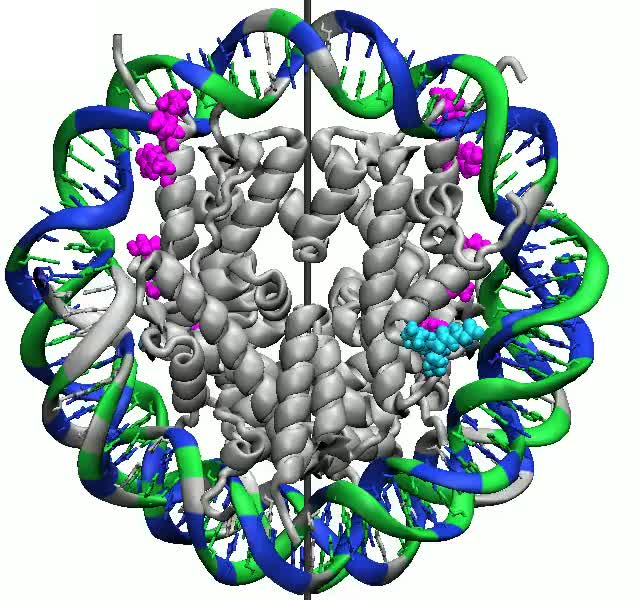
\includegraphics[width=1.0\linewidth]{cennuc/cennuc1}
\else
\animategraphics[autoplay,loop,width=1.0\linewidth,every=2]{10}{cennuc/cennuc}{1}{359}
\fi
\end{center}
\end{column}
\begin{column}{0.6\textwidth}  %%<--- here
\begin{center}
% \animategraphics[width=1.0\linewidth]{10}{10mus/10mus}{1}{100}

Задача: реконструкция структуры центромерной нуклеосомы пекарских дрожжей \textit{S. cerevisiae}.
\begin{itemize}
  \item На рисунке модель нуклеосомы третьей хромосомы дрожжей.
  \item Необычный сиквенс ДНК с А-траками функционально важен.
\end{itemize}
\end{center}
\end{column}
\end{columns}
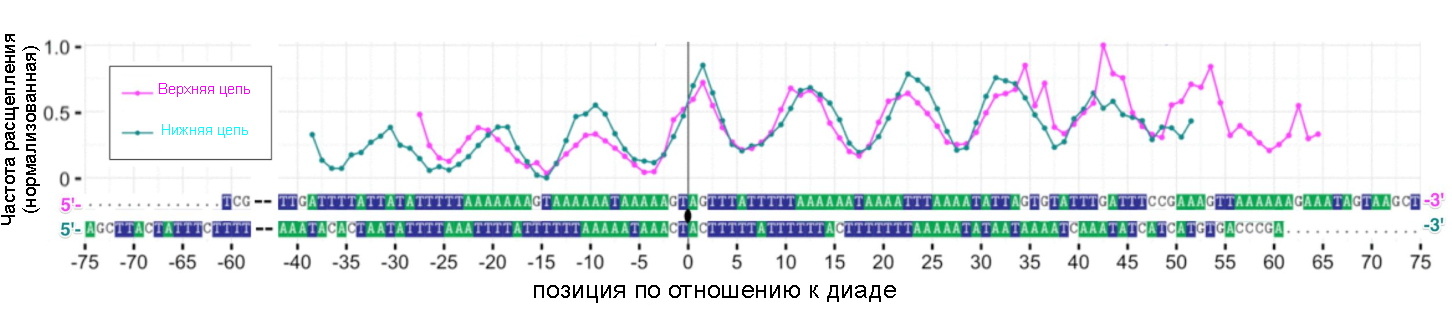
\includegraphics[width=1.0\textwidth]{s16b}
\note{Такой метод был использован нами, чтобы на основе известных структур нулеосомы и данных гидроксильного футпринтинга построить модель одной из центромерных нуклеосом пекарских дрожжей. После того, как определено положение ДНК, метод построения аналогичен методу построения моделей белков по гомологии. Точное позиционирование ДНК в модели важно для установления структуры поверхности, которая узнается белками кинетохоры. ДНК на нуклеосоме подобно винту (червячной передаче) трансляционное смещение на 1 нуклеотид сопряжено с ротационым поворотом на 36 градусов, что меняет конфигурацию поверхности узнаваемой белками. Известно, что для работы центромерных нуклеосом важны как особенности поверхности белка, так и сиквенс ДНК. (1-25)}
\end{frame}

\section[Глава 4]{Глава 4. Моделирование комплексов нуклеосом с белками хроматина.}

\begin{frame}
\frametitle{Проблема понимания супрануклеосомных структур}
\begin{columns}[t]
\begin{column}{0.5\textwidth}
\begin{center}
\underline{Огрубенное представление}
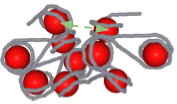
\includegraphics[width=1.0\textwidth]{s17l}
Хроматин в представлении бусин на нити. Красные шары - октамеры гистонов, синяя нить - ДНК.
\end{center}
\end{column}
\begin{column}{0.5\textwidth}  %%<--- here
\underline{Атомистическое представление}
\begin{center}
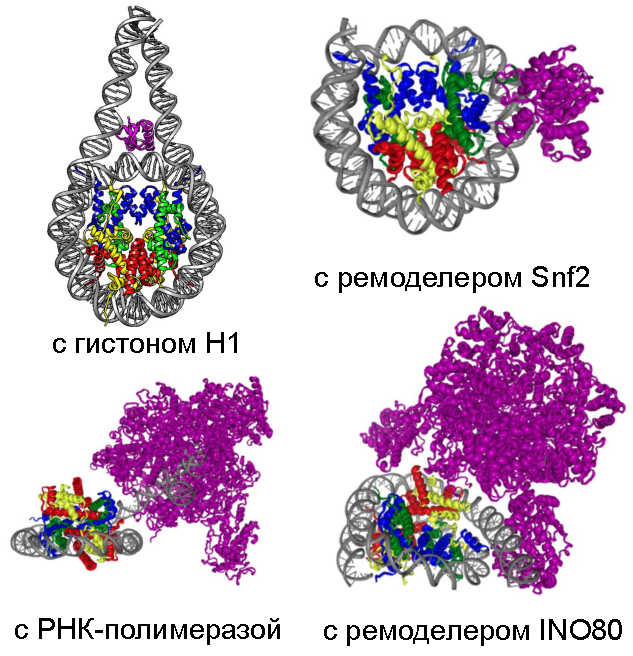
\includegraphics[width=1.0\textwidth]{s17r}
 % \begin{itemize}
 %        \item Ограниченные времена моделирования
 %        \item Времена функциональной динамики комплексов существенно больше
 %        \item Ограниченная точность силовых полей
 %        \item Чувствительность конформаций комплексов к точности параметров моделирования
 %    \end{itemize}
\end{center}
\end{column}
\end{columns}
\note{Следующая глава как раз посвящена изучению наднуклеосомной структуры. Это та инетересная область, где встречаются структурная биология и полимерная физика. С одной стороны возможно огрубленное описание как на рисунке слева. Данная модель построена путем огрубления случайных конформаций нуклеосом, полученных нами в МД, и их соединения прямыми участками ДНК. С другой стороны в хроматине присутвует большое количество белков взаимодействующих определенным образом с нуклеосомами и здесь необходимо учитывать и атомистическое представление. Из-за большого размера таких систем применение методов МД к ним затруднительно, однако можно применять различные интегративные и огрубленные подходы. (1-26)}
\end{frame}

\begin{frame}
\frametitle{Комплексы нуклеосом и РНК-полимераз}
\centering
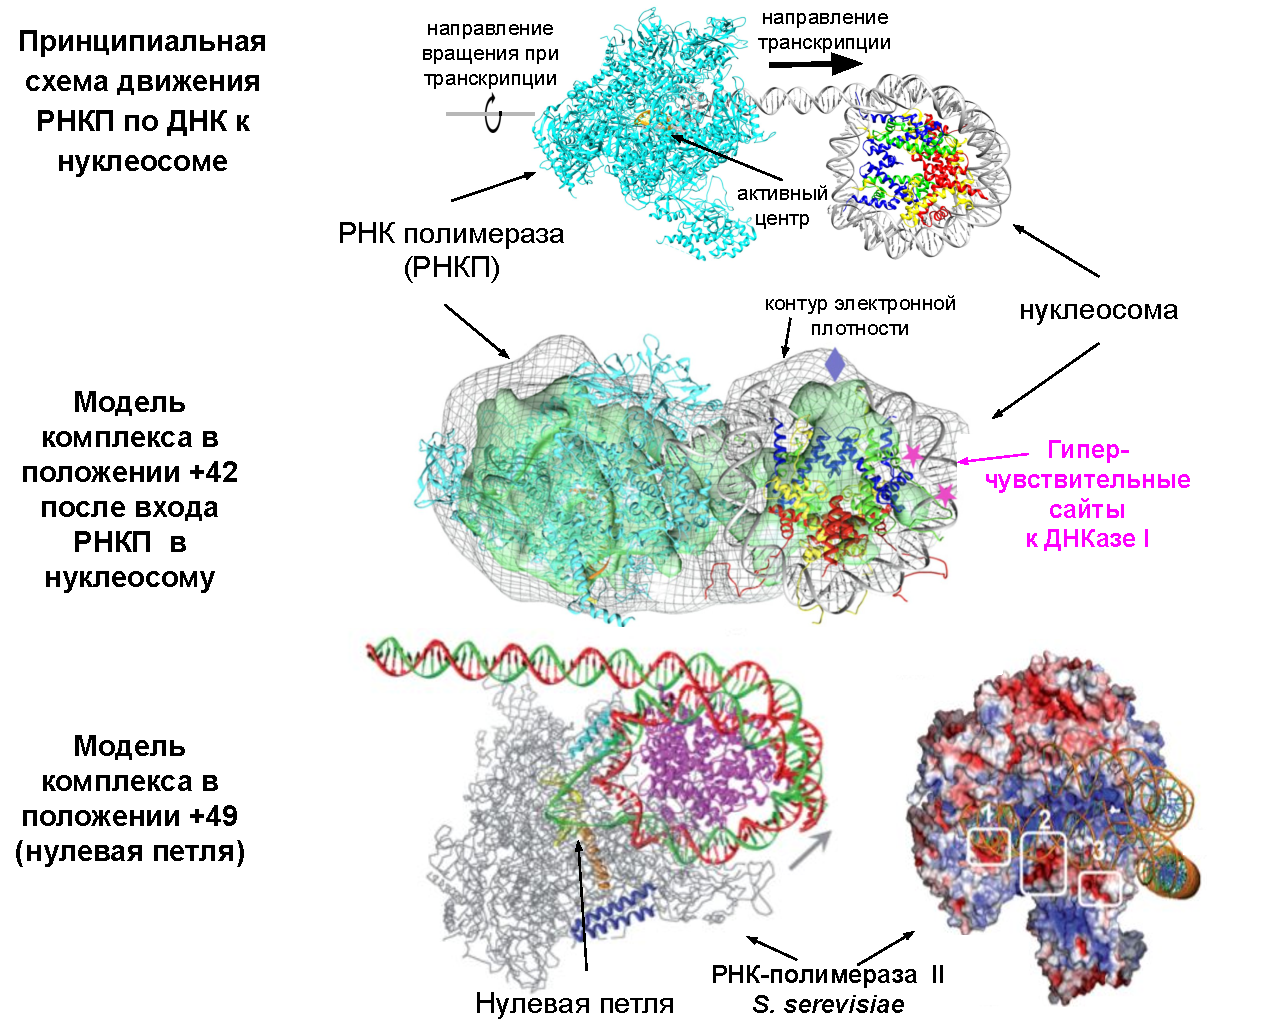
\includegraphics[height=0.9\textheight]{s18}
\note{На слайде представлен пример проведенного нами моделировния комплексов РНК полимеразы с нуклеосомой. РНК полимераза осуществляет считывание кода последовательности ДНК и синетз РНК. При этом она распрлетает ДНК и следует винтовой траектории ДНК. Возможность прохождения РНК вокруг нуклеосомы без ее разборки важно для сохранения эпигенетических меток. Здесь представлены модели структур нуклеосомы, когда ее активный сайт находится в $+42$ и $+49$ положении после входа в нуклеосому, построеные по данным футпринтинга и электронной микроскопии. Характерной особенность комплекса $+49$ ``нулевой петли'' является формирование полтного взаимодействия ДНК с гистонами как до, так и после полимеразы. Анализ электростатического потенциала указывает на то, что стабильности данного комплекса способствует наличие отрицательно заряженных остатков в местах контактов с положительно заряженными гистонами.(1.5-27.5)}
\end{frame}

\begin{frame}
\frametitle{Использование данных FRET}

\begin{columns}[t]
\begin{column}{0.5\textwidth}
\centering
Эффект Ферстеровского резонансного переноса энергии\\
\medskip
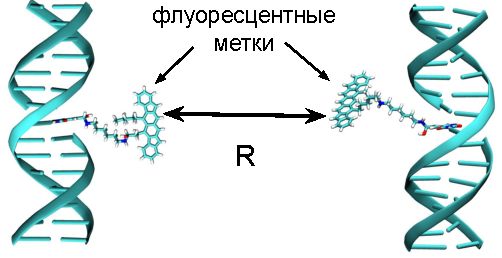
\includegraphics[width=1.0\textwidth]{s19l}

Эффективность переноса энергии с донора на акцептор

    $$E_{FRET}=\frac{1}{1+(R/R_0)^6}$$
    $R_0$ - радиус Ферстера
\end{column}
\begin{column}{0.5\textwidth}  %%<--- here



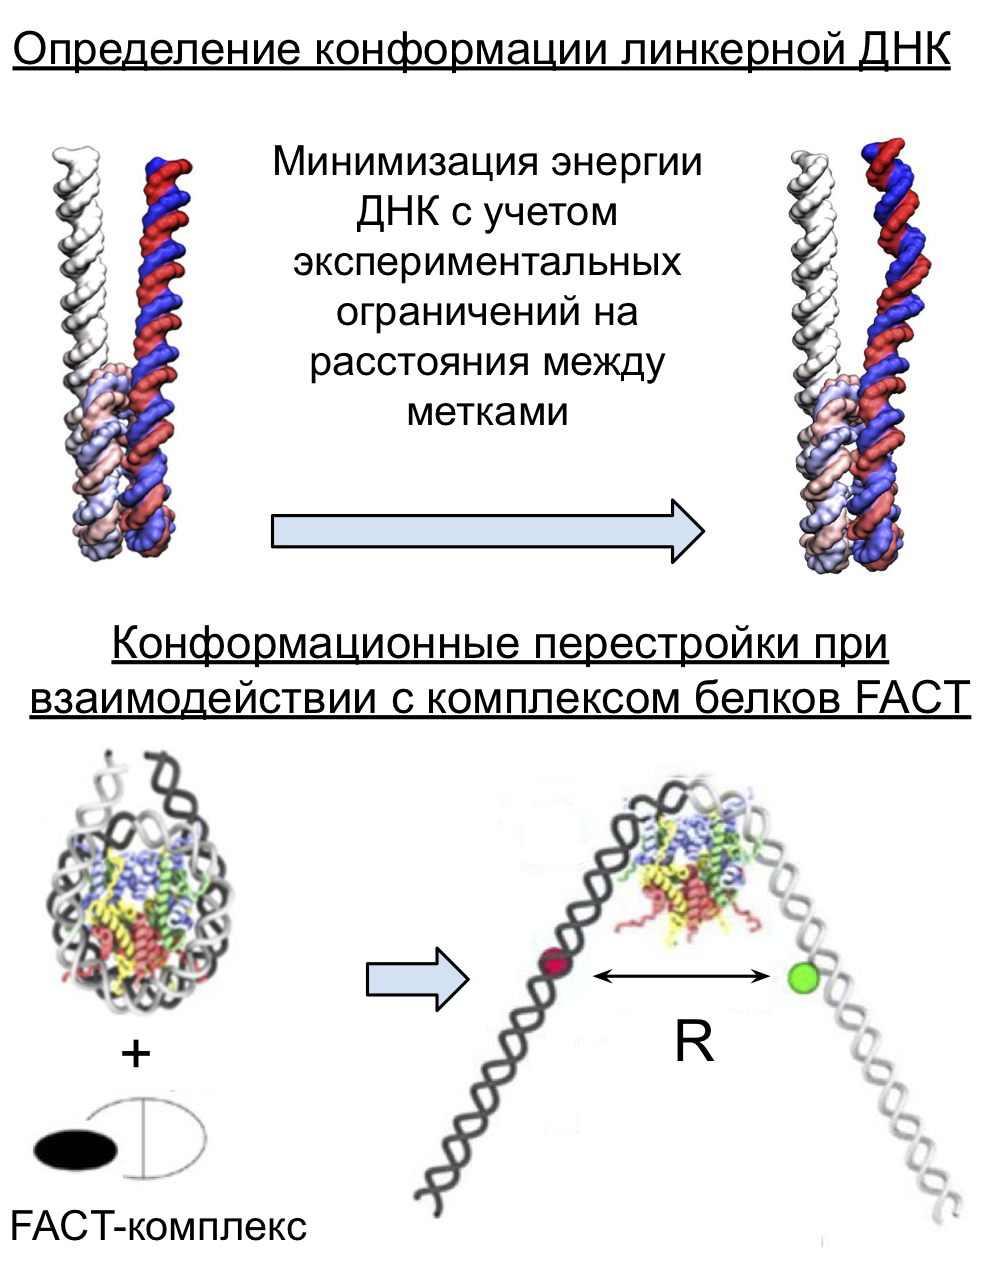
\includegraphics[width=1.0\textwidth]{s19r}
% \animategraphics[width=1.0\linewidth]{10}{10mus/10mus}{1}{100}

\end{column}
\end{columns}

\note{Еще одним видом данных, которые можно использовать для интегративного моделирования, являются данные экспериментов ФРЕТ. Эффект ФРЕТ возникает между двумя флуорестцентными метками, находящимися рядом с перектывающимися спектрами излучения и поглощения и заключается в безызлучательном переносе возбуждения с метки донора на метку акцептора. Регистрируя интенсивность данного эффекта спектроскопическими методами можно делать выводы о расстояниях между метками. Данные расстояния можно использовать для оптимизации и отбора огрубленных моделей молекулярных систем, соответствующих эксперименатльным данным. В работе нами такой подход использовался для построения моделей линкерных участков ДНК в нуклеосомах, а также для построения моделей разворачивания нуклеосом при из взаимодействии с комплексом белков FACT.(1-28.5)}
\end{frame}

\begin{frame}
\frametitle{Использование данных футпринтинга}
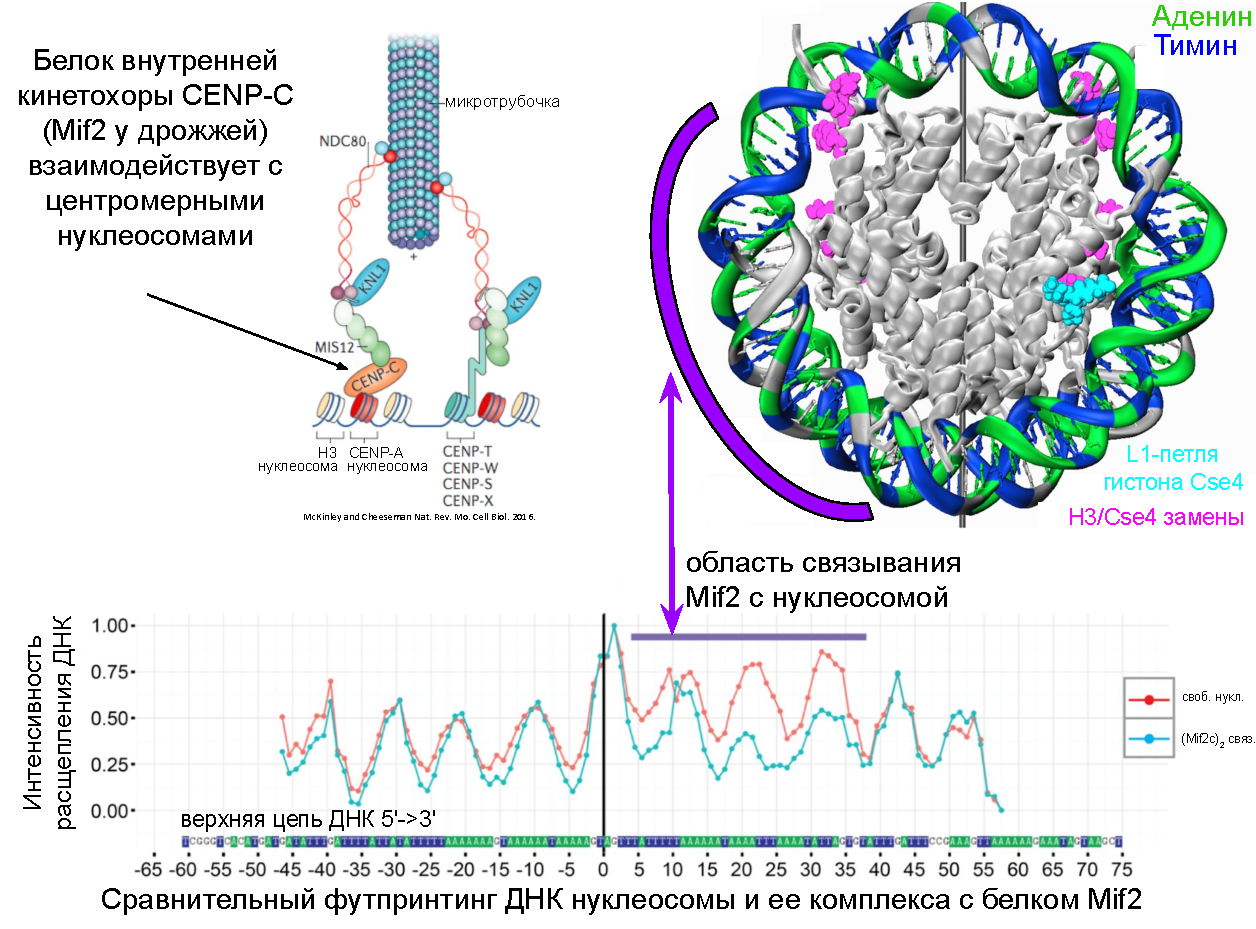
\includegraphics[height=0.9\textheight]{s20}
%\footfullcite{valieva_large-scale_2016}

\note{Метод гидроксильного футпринтинга также можно применять для изучения структуры комплексов нуклеосом с белками. На слайде ранее обсуждавшаяся построенная нами модель центромерной нуклеосомы пекарских дрожжей. С этой нуклеосомой взаимодействет белок CENP-C, который участвует в креплении центромеры к микротрубочкам. Сравнительная обработка экспериментов по футпринтингу чистых нуклеосом и нуклеосом в комплексе с этим белком позволила определить область связывания данного белка с нуклеосомой, отмеченную на рисунке. Как видно из ассиметрии профилей, особенности сиквенса ДНК и его позиционирования оказывают важными для связывания белка с одной стороны нуклеосомы, хотя существует и другая псевдосимметричная сторона.(1-29.5)}
\end{frame}


\section[Глава 5]{Глава 5. Интегративное моделирование амилоидоподобных фибрилл.}

\begin{frame}
\frametitle{Проблема понимания структуры амилоидных фибрилл}
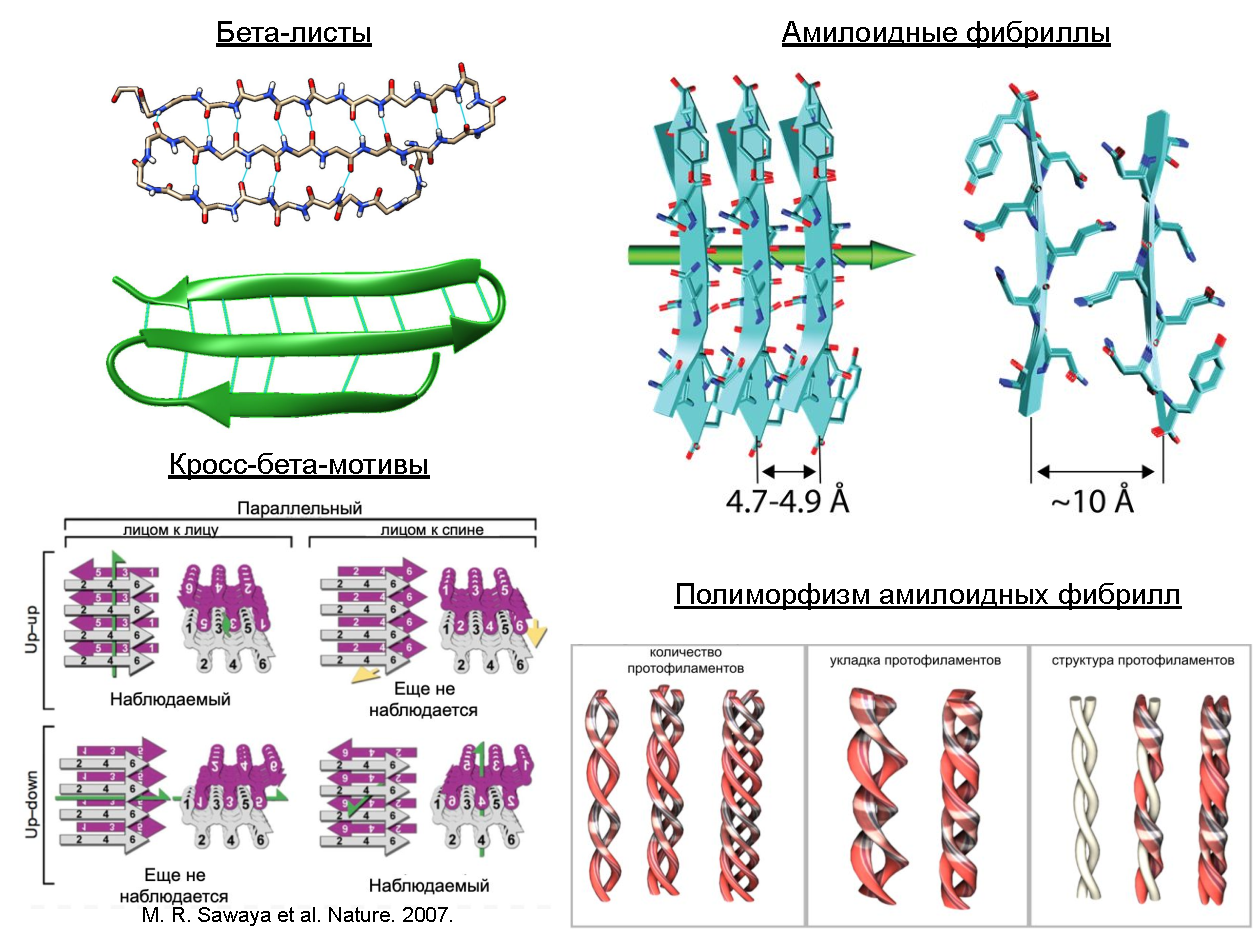
\includegraphics[height=0.9\textheight]{s21}
\note{В последней главе нами рассмотрены методы интегративного моделирвоания в применении к реконструкции амилоидоподобных фибрилл. Амилоидные фибриллы это комплексы, которые собираются из фрагментов белков или их пептидов путем их укладки в длинные бета-листы. Характерным является также взаимодействие бета-листов своими плоскостями и формирование так называемого кросс-бета-мотива, для которого характерна определенная периодичность видимая в экспериментах по рентгеновскому рассеянию. Важной особенностью фибрилл является их полиморфизм, как на уровне различных укладок бета-листов, так и на уровне агрегации и взаимодействия протофиломентов в более крупные фибриллы. Все это приводит к сложности в понимании структуры и свойств амилодоподобных фибрилл.(1-30.5)}
\end{frame}

\begin{frame}
\frametitle{Интегративный подход к моделированию фибрилл}
\centering
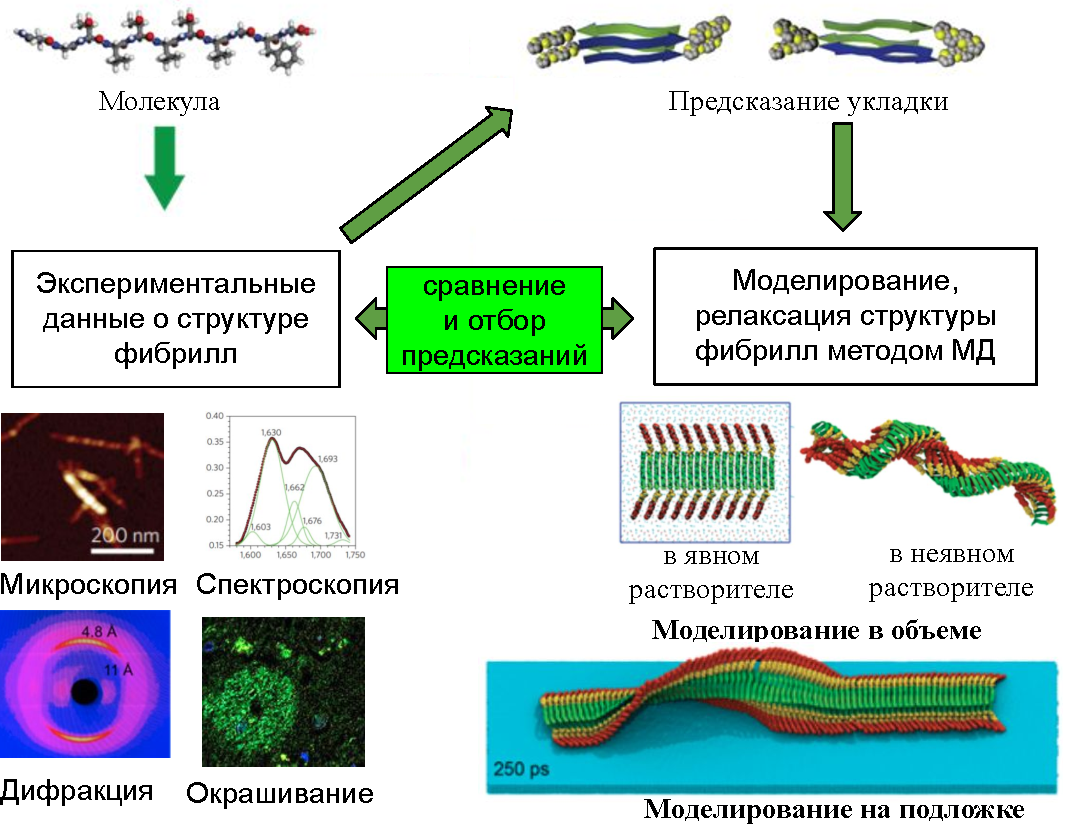
\includegraphics[height=0.85\textheight]{s22}
\note{Нами был предложен и разработан следующий интегративный подход. По экспериментальным данным с учетом различных методов молекулярного моделирования осуществляется предсказание возможных периодических укладок пептидов в фибриллах. К экспериментальным данным могут относится данные КД, ИК спектроскопии, рентгеновской дифракции и т.д. Затем на основе этих укладок конструируются модели фибрилл и проводится их релаксация и расчет методами МД в различных условиях. В результате фибриллы принимают свойственную им крупномасшатбную морфологию, которая стравнивается с данными микроскопии. (1-31.5)}
\end{frame}

\begin{frame}[allowframebreaks]
\frametitle{Нанопровода на основе амилоидоподобных фибрилл}
\centering
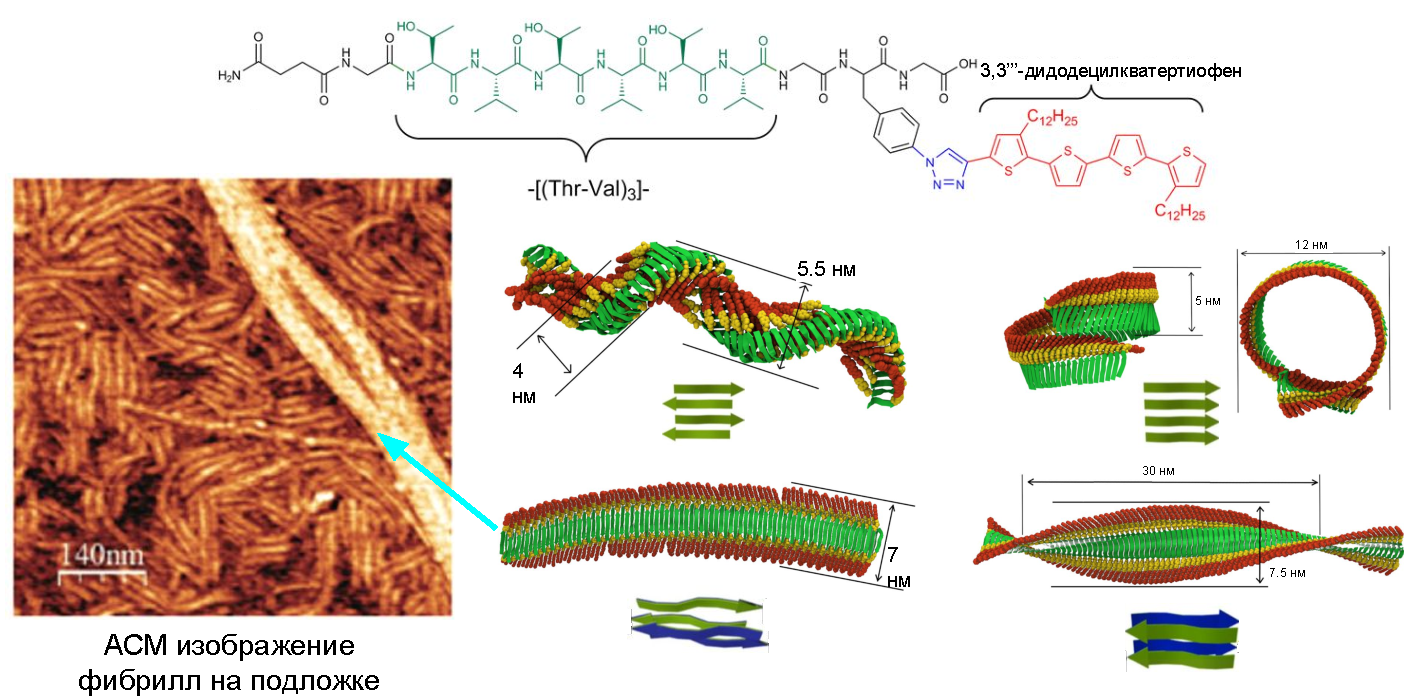
\includegraphics[width=1.0\textwidth]{s23}
\begin{center}
\ifdefined\HANDOUT
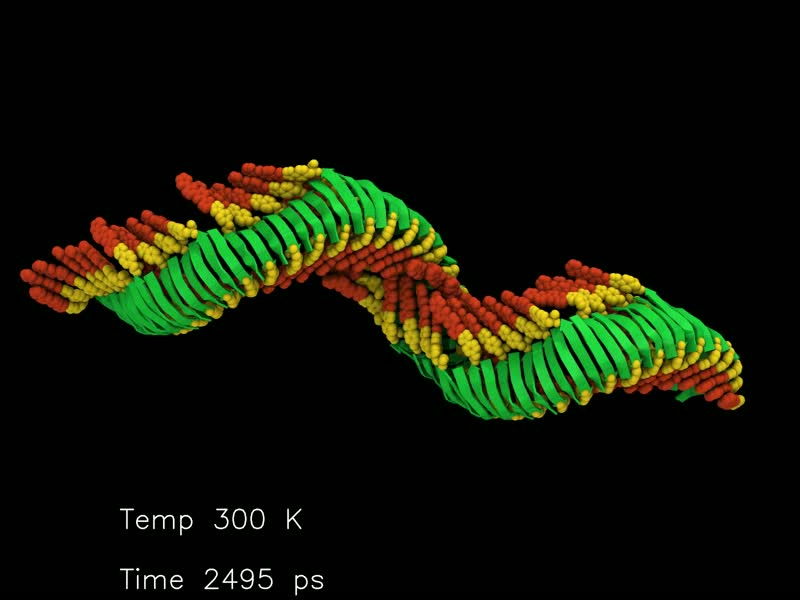
\includegraphics[height=0.75\textheight]{SL-AP/SL-AP500}
\else
\animategraphics[autoplay,height=0.75\textheight,every=2]{10}{SL-AP/SL-AP}{1}{500}
\fi\\
Релаксация начальной модели фибриллы методом МД. Температура поддерживается с помощью метода диссипативной динамики частиц.
\end{center}
\note{Такой подход был нами применен для выяснения структуры и дизайна фибрилл на основе гибридного соединения, состоящего из пептида и проводящего полимера тиофена. На слайде изображены различные укладки и соответвующие им морфологии, полученные в результате моделирования. В результате путем сопоставления изображений атомно-силовой микроскопии и моделей была выбрана наиболее вероятная укладка соответствующая двум анитипараллельным бета-листам, взаимодействующим своими гидрофобными поверхностями. На видео на этом слайде изображен процесс релаксации одной из начальных структур фибрилл. Для плавной резлаксации больших структур был разработан подход, основанный на поддержании постоянной температуры и моделировании неявного растоврителя с помощью метода диссипативной динамики частиц. (1.5-33)}
\end{frame}

\begin{frame}
\frametitle{Фибриллы EF-C из белка gp120}
\centering
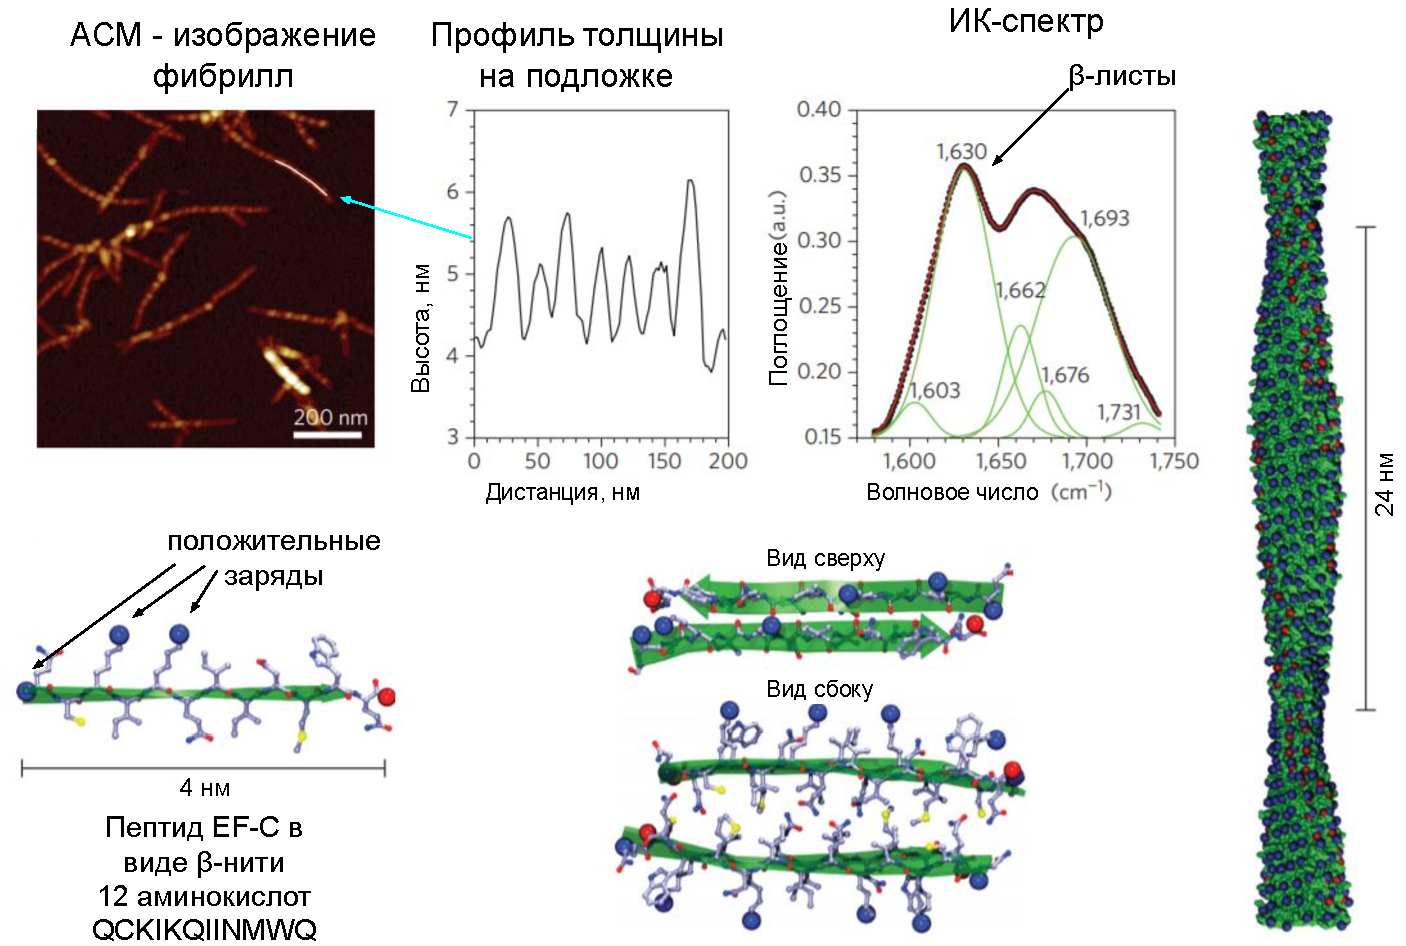
\includegraphics[height=0.85\textheight]{s24}
\note{Похожая задача была нами решена для построения стуруктуры фибрилл из пептидов, названных EF-C. Данные пептиды были выделены, как часть сиквенса гликопротеина gp120 ВИЧ-1. Экспериментально было установлено, что наличие данного пептида приводит к увеличению инфицирования клеток вирусом до 34 раз. На основе данных атомно-силовой микроскопии, кругового дихроизма, инфракрасной спектроскопии, порошковой дифракции рентгеновских лучей с применением разработанного нами интегративного подхода была построена молекулярная модель фибрилл EF-C. Установлено, что боковые цепи лизина образуют гидрофильную поверхность с высокой плотностью катионных зарядов при физиологическом pH. Таким образом фибриллы способствуют взаимодействию отрицательно заряженных поверхностей мембран вирусов с клетками, усиливая проникновение генетического материала вируса в клетку. (1.5-34.5)}
\end{frame}


%   \begin{frame}
% \frametitle{explanation}
% \begin{columns}
% \begin{column}{0.5\textwidth}
%    some text here some text here some text here some text here some text here
% \end{column}
% \begin{column}{0.5\textwidth}  %%<--- here
%     \begin{center}
     
%      \end{center}
% \end{column}
% \end{columns}
% \end{frame}



% \section{Списки}
% \begin{frame}[plain, noframenumbering]
%     \begin{center}
%         \Huge
%         Списки
%     \end{center}
% \end{frame}

% \subsection{Нумерованные}

% \begin{frame}
%     \frametitle{Нумерованные списки}
%     \begin{enumerate}
%         \item один
%         \item два
%         \item три
%     \end{enumerate}
% \end{frame}
% \note{
%     Этот текст будет виден только если его отображение включено
%     в~файле \textbf{Presentation/setup}.
%     Для раздельного вывода презентации и заметок на~разные экраны (как
%     в~impress или powerpoint) можно использовать программу
%     \textit{pdf-presenter-console}.
% }

% \subsection{Не нумерованные}


% \begin{frame}
%     \frametitle{Перечисления}
%     \begin{itemize}
%         \item Проблема 1
%         \item Проблема 2
%         \item Проблема 3
%     \end{itemize}
% \end{frame}
% \note[itemize]{
%     \item Тезис 1
%     \item Тезис 2
%     \item Тезис 3
% }

% \subsection{Комбинированные}

% \begin{frame}
%     \frametitle{Комбинация списков}
%     \begin{enumerate}
%         \item \textbf{Задача 1}
%               \begin{itemize}
%                   \item Подзадача 1-1
%                   \item Подзадача 1-2
%               \end{itemize}
%         \item \textbf{Задача 2}
%               \begin{itemize}
%                   \item Подзадача 2-1
%                   \item Подзадача 2-2
%                   \item Подзадача 2-3
%               \end{itemize}
%         \item \textbf{Задача 3}
%               \begin{itemize}
%                   \item Подзадача 3-1
%                   \item Подзадача 3-2
%                   \item Подзадача 3-3
%               \end{itemize}
%     \end{enumerate}
% \end{frame}
% \note[itemize]{
%     \item Задача 1
%     \item Задача 2
%     \item Задача 3
% }

% \begin{frame}[allowframebreaks]
%     \frametitle{Разделение слайда}
%     Поясняющий текст
%     \begin{itemize}
%         \item Один
%         \item Два
%         \item Три
%     \end{itemize}
%     \framebreak
%     Продолжение предыдущего слайда
% \end{frame}

% \section{Графика}
% \begin{frame}[plain, noframenumbering]
%     \begin{center}
%         \Huge
%         Графика
%     \end{center}
% \end{frame}


% \begin{frame}
%     \frametitle{Одиночное изображение}
%     \centering
%     
\includegraphics[width=0.8\linewidth]{latex} % окружение figure не требуется
% \end{frame}

% \begin{frame}
%     \frametitle{Векторная графика}
%     \begin{figure}
% 	    \centering
% 	    \ifdefmacro{\tikzsetnextfilename}{\tikzsetnextfilename{tikz_presentation}}{}% присваиваемое предкомпилированному pdf имя файла (не обязательно)
% 	    \begin{tikzpicture}
  \draw[<->,thick] (0,6) -- (0,0) -- (10,0); % axis
  \draw[help lines] (3,0) -- (3,5); % fill end
  \draw[help lines] (6,0) -- (6,5); % flattop end
  \draw[help lines] (9,0) -- (9,5); % decay end
  \draw[<->, thin] (0,5) -- (3,5); % fill
  \draw[<->, thin] (3,5) -- (6,5); % flattop
  \draw[<->, thin] (6,5) -- (9,5); % decay
  \draw[blue, ultra thick] (0,0) -- (0,4) -- (6,4) -- (6,0); % power
  \draw[red, ultra thick, domain=0:3] plot (\x, {4*(1 - exp(-1.5*\x))}); % fill plot
  \draw[red, ultra thick, domain=3:6] plot (\x, {4*(1 - exp(-1.5*\x))}); % flattop plot
  \draw[red, ultra thick, domain=6:9.5] plot (\x, {4*(1 - exp(-9)) - 4*(1 - exp(-1.5*\x+9))}); % decay plot
  \node [above] at (0,6) {\(E_{acc}\)};
  \node [right] at (10,0) {\(t\)};
  \node at (1.5,5.4) {заполнение};
  \node at (4.5,5.4) {работа};
  \node at (7.5,5.4) {затухание};
  \node at (4.5,1.4) {пучки};
  \foreach \x in {3.1,3.3,...,5.9} {
    \draw[->, green, thick] (\x,0) -- (\x,1);
  }
\end{tikzpicture}
%     \end{figure}
% \end{frame}

% \subsection{Расположение}

% \begin{frame}
%     \frametitle{Изображения по-вертикали}
%     \centering
%     \vfill
%     
\includegraphics[width=0.8\linewidth,height=0.1\textheight]{latex} \\
%     \TeX
%     \vfill
%     
\includegraphics[width=0.8\linewidth,height=0.2\textheight]{latex} \\
%     \LaTeX
%     \vfill
%     
\includegraphics[scale=0.2]{latex} \\
%     \vfill
% \end{frame}


% \begin{frame}
%     \frametitle{Изображения по-горизонтали}
%     \begin{minipage}[t]{0.47\linewidth}
%         \textbf{Составная \\ подпись 1}
%         \center{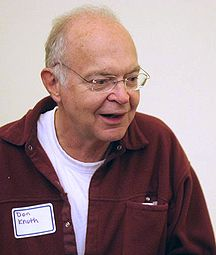
\includegraphics[width=1\linewidth]{knuth1}}
%     \end{minipage}
%     \hfill
%     \begin{minipage}[t]{0.47\linewidth}
%         \textbf{Составная \\ подпись 2}
%         \center{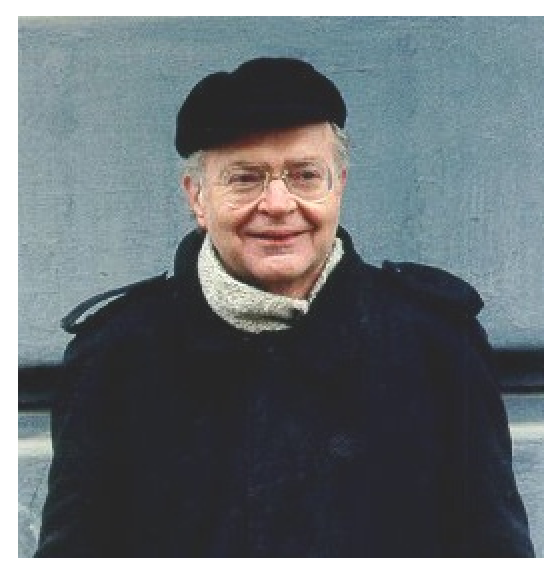
\includegraphics[width=1\linewidth]{knuth2}}
%     \end{minipage}
% \end{frame}

% \subsection{Линии}

% \begin{frame}
%     \frametitle{Разделяющие линии}
%     \begin{minipage}[c]{0.47\linewidth}
%         \center{
\includegraphics[width=1\linewidth]{latex}}
%         \bigskip
%         \hrule{}
%         \bigskip
%         \textbf{Составная \\ подпись 1}
%     \end{minipage}
%     \hfill
%     \vrule{}
%     \hfill
%     \begin{minipage}[c]{0.47\linewidth}
%         \flushright
%         \textbf{Составная \\ подпись 2}
%         \center{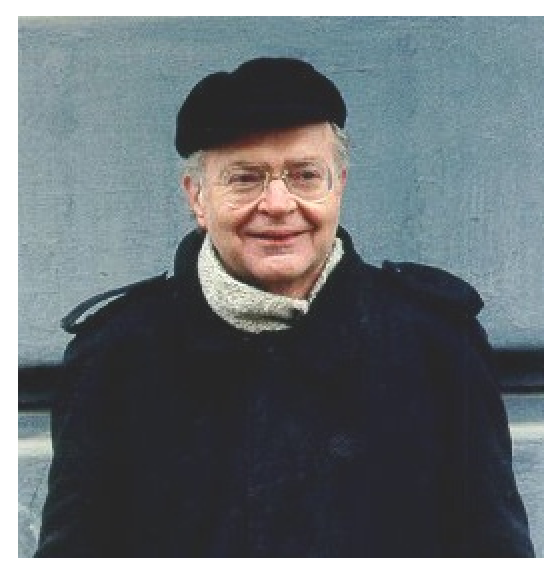
\includegraphics[width=1\linewidth]{knuth2}}
%     \end{minipage}
% \end{frame}

% \section{Остальное}
% \begin{frame}[plain, noframenumbering]
%     \begin{center}
%         \Huge
%         Остальное
%     \end{center}
% \end{frame}

% \subsection{Формулы}

% \begin{frame}
%     \frametitle{Формулы}
%     \[
%     \left\{
%     \begin{array}{rl}
%         \dot x = & \sigma (y-x)  \\
%         \dot y = & x (r - z) - y \\
%         \dot z = & xy - bz
%     \end{array}
%     \right.
%     \]
% \end{frame}

% \begin{frame}
%     \frametitle{amsmath}
%     \centering
%     \begin{minipage}[t]{0.5\linewidth}
%         \begin{multline*}
%             y = 1 x^1 + 2 x^2 + 3 x^3 + \\ + 4 x^4 + 5 x^5 + \dots
%         \end{multline*}
%     \end{minipage}
% \end{frame}

% \begin{frame}[allowframebreaks]
%     \frametitle{Уравнения Максвелла}
%     \centering{
%         \small
%         \def\arraystretch{1.8}%
%         \begin{tabular}{ll}
%             \toprule
%             Интегральная форма                                                                                                                                          & Дифференциальная форма                                                        \\ \midrule
%             \(Q_e(t) = \displaystyle\oiint_S \vec D(t) \cdot d\vec{s} = \displaystyle\iiint_V \rho_v(t) dv\)                                                              & \(\nabla \cdot \vec D(t) = \rho_v(t)\)                                          \\
%             \(\displaystyle\oiint_S \vec B(t) \cdot d\vec{s} = 0\)                                                                                                        & \(\nabla \cdot \vec B(t) = 0\)                                                  \\
%             \(V_{emf}(t) = \displaystyle\oint_L \vec E(t) \cdot d\vec{l}\) = \(- \displaystyle\iint_S \left[\frac{\partial\vec{B}(t)}{\partial t}\right] \cdot d\vec{s}\)   & \(\nabla \times \vec E(t) = - \frac{\partial\vec{B}(t)}{\partial t}\)           \\
%             \(I(t) = \displaystyle\oint_L \vec H(t) \cdot d\vec{l} = \displaystyle\iint_S \left[\vec J(t) + \frac{\partial\vec{D}(t)}{\partial t}\right] \cdot d\vec{s}\) & \(\nabla \times \vec H(t) = \vec J(t) + \frac{\partial\vec{D}(t)}{\partial t}\) \\ \midrule
%             \(\displaystyle\oiint_S \vec J \cdot d\vec{s} = -\frac{\partial Q_e}{\partial t}\)                                                                            & \(\nabla \cdot \vec J = - \frac{\partial \rho_v}{\partial t}\)                  \\
%             \bottomrule
%             \multicolumn{2}{c}{\(\vec D(t) = \left[\varepsilon(t)\right] * \vec E(t)\)}                                                                                                                                                                   \\
%             \multicolumn{2}{c}{\(\vec B(t) = \left[\mu(t)\right] * \vec H(t)\)}                                                                                                                                                                           \\
%         \end{tabular}
%     }
%     \framebreak

%     \hspace{0.05\linewidth}
%     \centering{
%         \small
%         \def\arraystretch{1.8}%
%         \begin{tabular}{ll}
%             \toprule
%             Интегральная форма                                                                                                            & Дифференциальная форма                             \\ \midrule
%             \(Q_e = \displaystyle\oiint_S \vec D \cdot d\vec{s} = \displaystyle\iiint_V \rho_v dv\)                                         & \(\nabla \cdot \vec D = \rho_v\)                     \\
%             \(\displaystyle\oiint_S \vec B \cdot d\vec{s} = 0\)                                                                             & \(\nabla \cdot \vec B = 0\)                          \\
%             \(V_{emf} = \displaystyle\oint_L \vec E \cdot d\vec{l}\) = \(- \displaystyle\iint_S \left[j \omega \vec B\right] \cdot d\vec{s}\) & \(\nabla \times \vec E = - j \omega \vec B\)         \\
%             \(I = \displaystyle\oint_L \vec H \cdot d\vec{l} = \displaystyle\iint_S \left[\vec J + j \omega \vec D\right] \cdot d\vec{s}\)  & \(\nabla \times \vec H = \vec J + j \omega \vec{D}\) \\ \midrule
%             \(\displaystyle\oiint_S \vec J \cdot d\vec{s} = - j \omega Q_e\)                                                                & \(\nabla \cdot \vec J = - j \omega \rho_v\)          \\
%             \bottomrule
%             \multicolumn{2}{c}{\(\vec D(t) = \left[\varepsilon\right] \vec E(t)\)}                                                                                                               \\
%             \multicolumn{2}{c}{\(\vec B(t) = \left[\mu\right] \vec H(t)\)}                                                                                                                       \\
%         \end{tabular}
%     }
% \end{frame}

% \subsection{Таблицы}

% \begin{frame}
%     \frametitle{Таблица}
%     \centering
%     \begin{tabular}{|l|l|}
%         \hline
%         \textbf{Заголовок 1} & \textbf{Заголовок 2} \\
%         \hline
%         Сумма                & \(b+a\)                \\
%         \hline
%         Разность             & \(a-b\)                \\
%         \hline
%         Произведение         & \(a*b\)                \\
%         \hline
%     \end{tabular}
% \end{frame}

% \begin{frame}
%     \frametitle{Другая таблица}
%     \centering
%     \begin{tabular}{lc}
%         \toprule
%         \multicolumn{1}{c}{\textbf{Заголовок 1}} & \textbf{Заголовок 2} \\ \midrule
%         Сумма                                    & \(b+a\)                \\
%         Разность                                 & \(a-b\)                \\
%         Произведение                             & \(a*b\)                \\
%         \bottomrule
%     \end{tabular}
% \end{frame}


% \subsection{Разное}

% \begin{frame}
%     \frametitle{Большой многоуровневый список}
%     \begin{itemize}
%         \item \textbf{Пункт 1}
%               \begin{itemize}
%                   \itemi Подпункт 1-1
%                   \itemi Подпункт 1-2
%               \end{itemize}
%         \item \textbf{Пункт 2}
%               \begin{itemize}
%                   \itemi Подпункт 2-1
%               \end{itemize}
%         \item \textbf{Пункт 3}
%               \begin{itemize}
%                   \itemi Подпункт 3-1
%                   \itemi Подпункт 3-2
%               \end{itemize}
%         \item \textbf{Пункт 4}
%               \begin{itemize}
%                   \itemi Подпункт 4-1
%               \end{itemize}
%         \item \textbf{Пункт 5}
%               \begin{itemize}
%                   \itemi Подпункт 5-1
%                   \itemi Подпункт 5-2
%                   \itemi Подпункт 5-3
%               \end{itemize}
%     \end{itemize}
% \end{frame}

% \begin{frame}
%     \frametitle{Четыре изображения}
%     \centering
%     
\includegraphics[width=0.35\linewidth,angle=35]{latex}
%     
\includegraphics[width=0.35\linewidth,angle=135]{latex}\\
%     
\includegraphics[width=0.35\linewidth,angle=15]{latex}
%     
\includegraphics[width=0.35\linewidth,angle=-15]{latex}
% \end{frame}

       % Настройки заглавной странице
\section{Заключение}
\subsection{Обсуждение результатов}
\begin{frame}
    \frametitle{Обсуждение результатов}
\begin{itemize}
 \item Метод МД является мощным инструментом, однако его применение ограничено вычислительными ресурсами и качеством параметризации моделей.
  Для преодоления ограничений можно использовать интегративное моделирование.

\item Логика построения интегративных подходов следующая. При моделировании структурных элементов и параметров системы, на структуру и значения которых может сильно повлиять неточность силовых полей, необходимо дополнительно привлекать экспериментальные данные. Вместе с тем, моделирование конформационно устойчивых структурных элементов можно производить на основании данных силовых полей. 

\item В интегративном моделировании весьма полезным походом является использования соображений структурной симметрии, мультимасштабный подоход с комбинацией атомистического и огрубленного представлений молекулярных систем.

\note{Перейдем к обсуждению результатов и заключению диссертационной работы. В резуьтате работы ... (1.5-36)}
\end{itemize}


\end{frame}

\subsection{Выводы работы}
\begin{frame}%[allowframebreaks]
    \frametitle{Выводы работы}

\begin{enumerate}
\justifying
\scriptsize
%\tiny
% \fontsize{5}{6}
\item Разработан интегративный подход и программные решения для мультимасштабного моделирования комплексов ДНК и белков, в котором используются различные данные экспериментов по ДНК футпринтингу, электронной микроскопии, FRET-микроскопии и комбинированное представление ДНК в атомистическом и в динуклеотидном приближении.



  \item В микросекундном временном диапазоне определены параметры крупномасштабных функциональных конформационных изменений структуры нуклеосом: вычислен ансамбль конформаций линкерной ДНК, установлено влияние электростатического отталкивания на геометрию сегментов линкерной ДНК, определено характерное время диссоциации концов нуклеосомальной ДНК от гистонового октамера (10 мкс), установлены флуктуационные структурные механизмы образования дефектов кручения ДНК, переключения конформаций гистоновых хвостов.



  \item Обработка экспериментальных данных по расщеплению ДНК гидроксильными радикалами (футпринтинга ДНК) позволила вычислить вероятность расщепления ДНК для каждого нуклеотида. Показано, что профили расщепления ДНК гидроксильными радикалами в нуклеосоме мало зависят от последовательности ДНК, и определяются в основном позиционированием ДНК на нуклеосоме. Предложен алгоритм точного определения положения ДНК в нуклеосоме по данным футпринтинга для двух цепей ДНК на основании положения оси псевдосимметрии.

\end{enumerate}
\end{frame}

\begin{frame}%[allowframebreaks]
    \frametitle{Выводы работы (продолжение)}

\begin{enumerate}
\justifying
\scriptsize
%\tiny
% \fontsize{5}{6}

  \item С помощью методов интегративного моделирования были установлены структуры и параметры взаимодействий комплексов нуклеосом с РНК полимеразами, белком CENP-C, гистоном H1, белками комплекса FACT. Установлено, что в положении +49 после входа в нуклеосому РНК полимераза II может формировать компактный комплекс с нуклеосомой, в котором контакты гистонов с ДНК сохраняются по обе стороны активного центра. В модели центромерной нуклеосомы дрожжей определено положение ДНК и установлено, что белок CENP-C взаимодействует с нуклеосомой в районе 20 нуклеотидов от центра симметрии нуклеосомы. Предложены модели конформации линкерных сегментов ДНК при связывании гистона H1.  Установлены амплитуды конформационной подвижности ДНК в нуклеосомах при связывании с комплексом FACT.
  

 \item Разработанные подходы построения моделей амилоидоподобных фибрилл позволили изучить связь взаимного расположения пептидов в фибриллярных структурах с крупномасштабной морфологией амилоидоподобных фибрилл и таким образом установить структурную организацию филаментов на основе диблок олигомеров кватертиофена и пептида $(Thr-Val)_3$, а также на основе фрагмента белка gp120. Установлено, что рассмотренные амилоидоподобные фибриллы могут образовываться на основе двух взаимодействующих бета-листов, которые формируют либо плоскую ленту, либо левозакрученную ленту с периодом 24-30 нм.

\end{enumerate}
\end{frame}

% \begin{frame}
%     \frametitle{Научная новизна}
%     \begin{itemize}
%         \item Впервые реализован \dots
%         \item Разработана программа \dots
%         \item Впервые проведён анализ \dots
%         \item Предложена схема \dots
%     \end{itemize}
% \end{frame}
% \note{
%     Проговаривается вслух научная новизна
% }

% \begin{frame}
%     \frametitle{Научная и практическая значимость}
%     \begin{itemize}
%         \item Получены выражения для \dots.
%         \item Определены условия \dots.
%         \item Разработаны устройства \dots.
%     \end{itemize}
% \end{frame}
% \note{
%     Проговариваются вслух научная и практическая значимость
% }

% \begin{frame}
%     \frametitle{Свидетельство о регистрации программы}
%     \begin{figure}[h]
%         \centering
%         
\includegraphics[height=0.7\textheight]{registration}
%     \end{figure}
% \end{frame}
% \note{
%     Получено свидетельство о регистрации разработанной программы \textsc{Hello~world™}.
% }

% \begin{frame}
%     \frametitle{Акт о внедрении}
%     \begin{figure}[h]
%         \centering
%         \fbox{
%             \begin{minipage}[t]{0.4\linewidth}
%                 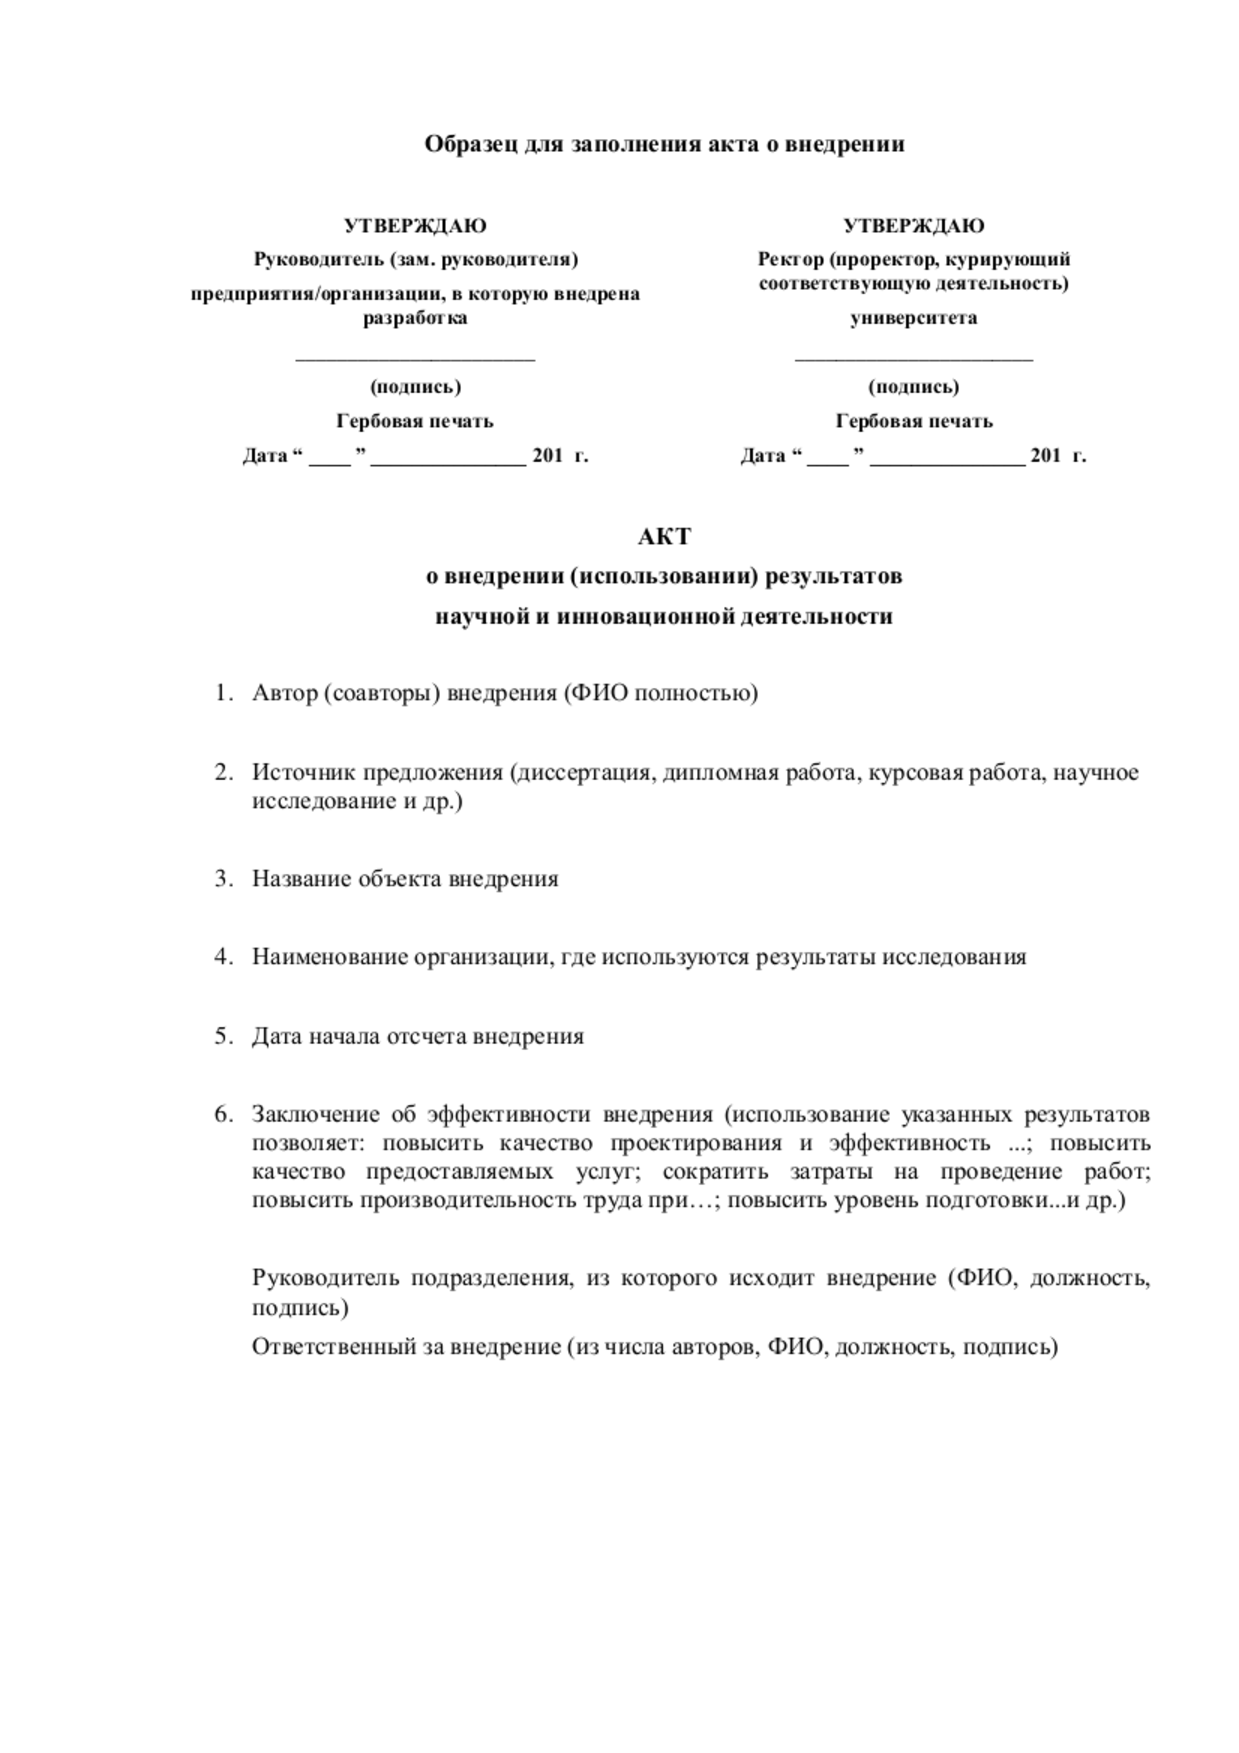
\includegraphics[width=\linewidth]{implementation}
%             \end{minipage}
%         }
%     \end{figure}
% \end{frame}
% \note{
%     Получен акт о внедрении.
% }
\subsection{Основные публикации}
\begin{frame}[allowframebreaks] % публикации на одной странице
% \begin{frame}[t,allowframebreaks] % публикации на нескольких страницах
    \frametitle{Основные публикации}
% \nocite{hada_histone_2019,bass_effect_2019,armeev_linking_2019,shaytan_structural_2018,gorkovets_joint_2018,xiao_molecular_2017,shaytan_hydroxyl-radical_2017,gribkova_investigation_2017,el_kennani_ms_histonedb_2017,chertkov_dual_2017,armeev_modeling_2016,armeev_nucleosome_2016,biswas_genomic_2016,draizen_histonedb_2016,lyubitelev_structure_2016,shaitan_dynamics_2016,shaytan_coupling_2016,shaytan_trajectories_2016,valieva_large-scale_2016,armeev_conformational_2015,armeev_molecular_2015,frank_direct_2015,gaykalova_structural_2015,goncearenco_structural_2015,shaytan_nucleosome_2015,bozdaganyan_comparative_2014,chang_analysis_2014,kasimova_voltage-gated_2014,nishi_physicochemical_2014,sokolova_genome_2014,yolamanova_peptide_2013,shaitan_influence_2013,orekhov_calculation_2012,shaytan_self-assembling_2011,shaytan_self-organizing_2011}
% \renewcommand*{\bibfont}{\normalfont\scriptsize}
% %\renewcommand\bibliographytypesize{\small}
%     \ifnumequal{\value{bibliosel}}{0}{
%         \insertbiblioauthor
%     }{
%         \printbibliography%
%     }

\setbeamertemplate{enumerate items}[default]
\setbeamercolor*{enumerate item}{fg=black}
\scriptsize
\begin{enumerate}
 \justifying

 \item Histone Octamer Structure Is Altered Early in ISW2 ATP-Dependent Nucleosome Remode-ling / A. Hada, S. K. Hota, J. Luo, Y.-c. Lin, S. Kale, A. K. Shaytan, S. K. Bhardwaj, [et al.] // Cell Reports. –– 2019. –– July 2. –– Vol. 28, no. 1. –– 282––294.e6. –– DOI: 10.1016/j.celrep.2019. 05.106. –– \textbf{IF WoS 7.7} - (2,3/0,3).
\item The Effect of Oncomutations and Posttranslational Modifications of Histone H1 on Chroma-tosome Structure and Stability / M. V. Bass, G. A. Armeev, K. V. Shaitan, A. K. Shaytan // Moscow University Biological Sciences Bulletin. –– 2019. –– July. –– Vol. 74, no. 3. –– P. 121––126. –– DOI: 10.3103/S0096392519030015. –– \textbf{IF RINC 0.76} - (0,7/0,3).
\item  Linking Chromatin Composition and Structural Dynamics at the Nucleosome Level / G. A. Armeev, A. K. Gribkova, I. Pospelova, G. A. Komarova, A. K. Shaytan // Current Opinion in Structural Biology. –– 2019. –– June. –– Vol. 56. –– P. 46––55. –– DOI: 10.1016/j.sbi. 2018.11.006. –– \textbf{IF WoS 6.908} - (1,2/0,6).
\item  Structural Interpretation of DNA–Protein Hydroxyl-Radical Footprinting Experiments with High Resolution Using HYDROID / A. K. Shaytan, H. Xiao, G. A. Armeev, D. A. Gaykalova, G. A. Komarova, C. Wu, V. M. Studitsky, D. Landsman, A. R. Panchenko // Nature Protocols. –– 2018. –– Nov. –– Vol. 13, no. 11. –– P. 2535––2556. –– DOI: 10.1038/s41596-018-0048-z. –– \textbf{IF WoS 11.334} - (2,5/2,2).
\item  Joint Effect of Histone H1 Amino Acid Sequence and DNA Nucleotide Sequence on the Structure of Chromatosomes: Analysis by Molecular Modeling Methods / T. K. Gorkovets, G. A. Armeev, K. V. Shaitan, A. K. Shaytan // Moscow University Biological Sciences Bulletin. –– 2018. –– Apr. –– Vol. 73, no. 2. –– P. 82––87. –– DOI: 10 . 3103 / S0096392518020025. –– \textbf{IF RINC 0.76} - (0,7/0,3).
\item  Molecular Basis of CENP-C Association with the CENP-A Nucleosome at Yeast Centromeres / H. Xiao, F. Wang, J. Wisniewski, A. K. Shaytan, R. Ghirlando, P. C. FitzGerald, Y. Huang, [et al.] // Genes \& Development. –– 2017. –– Oct. 1. –– Vol. 31, no. 19. –– P. 1958––1972. –– DOI: 10.1101/gad.304782.117. –– \textbf{IF WoS 9.527} - (1,7/0,3).
\item  Hydroxyl-Radical Footprinting Combined with Molecular Modeling Identifies Unique Features of DNA Conformation and Nucleosome Positioning / A. K. Shaytan, H. Xiao, G. A. Armeev, C. Wu, D. Landsman, A. R. Panchenko // Nucleic Acids Research. –– 2017. –– Sept. 19. –– Vol. 45, no. 16. –– P. 9229––9243. –– DOI: 10.1093/nar/gkx616. –– \textbf{IF WoS 11.501} - (1,7/1,5).
\item  Gribkova, A. K. Investigation of Histone-DNA Binding Energy as a Function of DNA Unwrapping from Nucleosome Using Molecular Modeling / A. K. Gribkova, G. A. Armeev, A. K. Shaytan // Moscow University Biological Sciences Bulletin. –– 2017. –– July. –– Vol. 72, no. 3. –– P. 142––145. –– DOI: 10.3103/S009639251703004X. –– \textbf{IF RINC 0.76} - (0,5/0,2).
\item  MS\_HistoneDB, a Manually Curated Resource for Proteomic Analysis of Human and Mouse Histones / S. El Kennani, A. Adrait, A. K. Shaytan, S. Khochbin, C. Bruley, A. R. Panchenko, D. Landsman, D. Pflieger, J. Govin // Epigenetics \& Chromatin. –– 2017. –– Dec. –– Vol. 10, no. 1. –– DOI: 10.1186/s13072-016-0109-x. –– \textbf{IF WoS 5.333} - (2,1/0,5).
\item  Dual Active Site in the Endolytic Transglycosylase Gp144 of Bacteriophage phiKZ / O. V. Chertkov, G. A. Armeev, I. V. Uporov, S. A. Legotsky, N. N. Sykilinda, A. K. Shaytan, N. L. Klyachko, K. A. Miroshnikov // Acta Naturae. –– 2017. –– Vol. 9, no. 1. –– P. 7. –– DOI: 10.32607/20758251-2017-9-1-81-87. –– \textbf{IF WoS 1.62} - (0,8/0,1).
\item  Modeling of the Structure of Protein–DNA Complexes Using the Data from FRET and Footprinting Experiments / G. A. Armeev, T. K. Gorkovets, D. A. Efimova, K. V. Shaitan, A. K. Shaytan // Moscow University Biological Sciences Bulletin. –– 2016. –– Jan. –– Vol. 71, no. 1. –– P. 29––33. –– DOI: 10.3103/S0096392516010016. –– \textbf{IF RINC 0.76} - (0,6/0,2).
\item  Armeev, G. A. Nucleosome Structure Relaxation during DNA Unwrapping: Molecular Dynamics Simulation Study / G. A. Armeev, K. V. Shaitan, A. K. Shaytan // Moscow University Biological Sciences Bulletin. –– 2016. –– July. –– Vol. 71, no. 3. –– P. 141––144. –– DOI: 10.3103/S0096392516030020. –– \textbf{IF RINC 0.76} - (0,5/0,2).
 \item  Genomic Profiling of Multiple Sequentially Acquired Tumor Metastatic Sites from an “Exceptional Responder” Lung Adenocarcinoma Patient Reveals Extensive Genomic Hetero-geneity and Novel Somatic Variants Driving Treatment Response / R. Biswas, S. Gao, C. M. Cultraro, T. K. Maity, A. Venugopalan, Z. Abdullaev, A. K. Shaytan, [et al.] // Molecular Case Studies. –– 2016. –– Nov. –– Vol. 2, no. 6. –– a001263. –– DOI: 10.1101/mcs.a001263. –– \textbf{IF WoS 1.750} - (3,1/0,5).
 \item  HistoneDB 2.0: A Histone Database with Variants—an Integrated Resource to Explore Histones and Their Variants / E. J. Draizen, A. K. Shaytan, L. Marino-Ramirez, P. B. Talbert, D. Landsman, A. R. Panchenko // Database. –– 2016. –– Vol. 2016. –– baw014. –– DOI: 10.1093/database/baw014. –– \textbf{IF WoS 2.593} - (1,2/0,6).
 \item  Structure and Functions of Linker Histones / A. V. Lyubitelev, D. V. Nikitin, A. K. Shaytan, V. M. Studitsky, M. P. Kirpichnikov // Biochemistry (Moscow). –– 2016. –– Mar. –– Vol. 81, no. 3. –– P. 213––223. –– DOI: 10.1134/S0006297916030032. –– \textbf{IF WoS 1.978} - (1,3/0,1).
 \item  Shaitan, K. V. The Dynamics of Irreversible Evaporation of a Water–Protein Droplet and the Problem of Structural and Dynamic Experiments with Single Molecules / K. V. Shaitan, G. A. Armeev, A. K. Shaytan // Biophysics. –– 2016. –– Mar. –– Vol. 61, no. 2. –– P. 177––184. –– DOI: 10.1134/S0006350916020172. –– \textbf{IF SJR 0.226} - (0,9/0,1).
 \item  Coupling between Histone Conformations and DNA Geometry in Nucleosomes on a Micro-second Timescale: Atomistic Insights into Nucleosome Functions / A. K. Shaytan, G. A. Armeev, A. Goncearenco, V. B. Zhurkin, D. Landsman, A. R. Panchenko // Journal of Molecular Biology. –– 2016. –– Jan. –– Vol. 428, no. 1. –– P. 221––237. –– DOI: 10.1016/j.jmb.2015.12.004. –– \textbf{IF WoS 5.04} - (2,0/1,8).
 \item  Trajectories of Microsecond Molecular Dynamics Simulations of Nucleosomes and Nucleo-some Core Particles / A. K. Shaytan, G. A. Armeev, A. Goncearenco, V. B. Zhurkin, D. Landsman, A. R. Panchenko // Data in Brief. –– 2016. –– June. –– Vol. 7. –– P. 1678––1681. –– DOI: 10.1016/j.dib.2016.04.073. –– \textbf{IF WoS 0.97} - (0,5/0,5).
 \item  Large-Scale ATP-Independent Nucleosome Unfolding by a Histone Chaperone / M. E. Valieva, G. A. Armeev, K. S. Kudryashova, N. S. Gerasimova, A. K. Shaytan, O. I. Kulaeva, L. L. McCullough, [et al.] // Nature Structural \& Molecular Biology. –– 2016. –– Dec. –– Vol. 23, no. 12. –– P. 1111––1116. –– DOI: 10.1038/nsmb.3321. –– \textbf{IF WoS 11.98} - (0,9/0,1).
 \item  Armeev, G. A. Conformational Flexibility of Nucleosomes: A Molecular Dynamics Study / G. A. Armeev, K. V. Shaitan, A. K. Shaytan // Moscow University Biological Sciences Bulletin. –– 2015. –– July. –– Vol. 70, no. 3. –– P. 147––151. –– DOI: 10.3103/S009639251- 5030025. –– \textbf{IF RINC 0.76} - (0,6/0,3).
 \item  Armeev, G. A. Molecular Dynamics Study of the Ionic Environment and Electrical Character-istics of Nucleosomes / G. A. Armeev, K. V. Shaitan, A. K. Shaitan // Moscow University Biological Sciences Bulletin. –– 2015. –– Oct. –– Vol. 70, no. 4. –– P. 173––176. –– DOI: 10.3103/ S0096392515040033. –– \textbf{IF RINC 0.76} - (0,5/0,2).
 \item  Direct Prediction of Residual Dipolar Couplings of Small Molecules in a Stretched Gel by Stochastic Molecular Dynamics Simulations: Direct Prediction of Residual Dipolar Couplings by Stochastic MD Simulations / A. O. Frank, J. C. Freudenberger, A. K. Shaytan, H. Kessler, B. Luy // Magnetic Resonance in Chemistry. –– 2015. –– Mar. –– Vol. 53, no. 3. –– P. 213––217. –– DOI: 10.1002/mrc.4181. –– \textbf{IF WoS 1.731} - (0,6/0,1).
 \item  Structural Analysis of Nucleosomal Barrier to Transcription / D. A. Gaykalova, O. I. Kulaeva, O. Volokh, A. K. Shaytan, F.-K. Hsieh, M. P. Kirpichnikov, O. S. Sokolova, V. M. Studitsky // Proceedings of the National Academy of Sciences. –– 2015. –– Oct. 27. –– Vol. 112,
no. 43. –– E5787––E5795. –– DOI: 10.1073/pnas.1508371112. –– \textbf{IF WoS 9.412} - (1,0/0,3).
 \item  Structural Perspectives on the Evolutionary Expansion of Unique Protein-Protein Binding Sites / A. Goncearenco, A. K. Shaytan, B. A. Shoemaker, A. R. Panchenko // Biophysical Journal. –– 2015. –– Sept. –– Vol. 109, no. 6. –– P. 1295––1306. –– DOI: 10.1016/j.bpj.2015. 06.056. –– \textbf{IF WoS 3.665} - (1,4/0,4).
 \item  Shaytan, A. K. Nucleosome Adaptability Conferred by Sequence and Structural Variations in Histone H2A-H2B Dimers / A. K. Shaytan, D. Landsman, A. R. Panchenko // Current Opinion in Structural Biology. –– 2015. –– June. –– Vol. 32. –– P. 48––57. –– DOI: 10.1016/j.sbi. 2015.02.004. –– \textbf{IF WoS 6.908} - (1,2/1,0).
 \item  Comparative Computational Study of Interaction of C60-Fullerene and Tris-Malonyl-C60- Fullerene Isomers with Lipid Bilayer: Relation to Their Antioxidant Effect / M. E. Bozdaga-nyan, P. S. Orekhov, A. K. Shaytan, K. V. Shaitan // PLoS ONE / ed. by C. M. Soares. –– 2014. –– July 14. –– Vol. 9, no. 7. –– e102487. –– DOI: 10.1371/journal. pone.0102487. –– \textbf{IF WoS 2.740} - (0,9/0,1).
 \item  Analysis of the Mechanism of Nucleosome Survival during Transcription / H.-W. Chang, O. I. Kulaeva, A. K. Shaytan, M. Kibanov, K. Kuznedelov, K. V. Severinov, M. P. Kirpichnikov, D. J. Clark, V. M. Studitsky // Nucleic Acids Research. –– 2014. –– Feb. –– Vol. 42,
no. 3. –– P. 1619––1627. –– DOI: 10 . 1093 / nar / gkt1120. –– \textbf{IF WoS 11.501} - (1,0/0,2).
 \item  Voltage-Gated Ion Channel Modulation by Lipids: Insights from Molecular Dynamics Simulations / M. A. Kasimova, M. Tarek, A. K. Shaytan, K. V. Shaitan, L. Delemotte // Biochimica et Biophysica Acta (BBA) - Biomembranes. –– 2014. –– May. –– Vol. 1838, no. 5. –– P. 1322––1331. –– DOI: 10.1016/j.bbamem.2014.01.024. –– \textbf{IF WoS 3.4} - (1,2/0,1).
 \item  Nishi, H. Physicochemical Mechanisms of Protein Regulation by Phosphorylation / H. Nishi, A. Shaytan, A. R. Panchenko // Frontiers in Genetics. –– 2014. –– Aug. 7. –– Vol. 5. –– DOI: 10.3389/fgene.2014. 00270. –– \textbf{IF WoS 3.789} - (1,2/0,4).
 \item  Genome Packaging in EL and Lin68, Two Giant phiKZ-like Bacteriophages of P. Aeruginosa / O. Sokolova, O. Shaburova, E. Pechnikova, A. Shaytan, S. Krylov, N. Kiselev, V. Krylov // Virology. –– 2014. –– Nov. –– Vol. 468––470. –– P. 472––478. –– DOI: 10.1016/j.virol.2014.09. 002. –– \textbf{IF WoS 2.464} - (0,8/0,1).
 \item  Peptide Nanofibrils Boost Retroviral Gene Transfer and Provide a Rapid Means for Concent-rating Viruses / M. Yolamanova, C. Meier, A. K. Shaytan, V. Vas, C. W. Bertoncini, F. Arnold, O. Zirafi, [et al.] // Nature Nanotechnology. –– 2013. –– Feb. –– Vol. 8, no. 2. –– P. 130––136. –– DOI: 10.1038/nnano.2012.248. –– \textbf{IF WoS 31.538} - (0,8/0,2).
 \item  Influence of Interionic Interactions on Functional State and Blocker Binding of Voltage-Gated Potassium Channels / K. V. Shaitan, O. S. Sokolova, A. K. Shaitan, M. A. Kasimova, V. N. Novoseletskii, M. P. Kirpichnikov // Moscow University Biological Sciences Bulletin. –– 2013. –– Mar. –– Vol. 68, no. 1. –– P. 8––14. –– DOI: 10.3103/S009639251301- 0057. –– \textbf{IF RINC 0.76} - (0,8/0,1).
 \item  Orekhov, P. S. Calculation of Spectral Shifts of the Mutants of Bacteriorhodopsin by QM/MM Methods / P. S. Orekhov, A. K. Shaytan, K. V. Shaitan // Biophysics. –– 2012. –– Mar. –– Vol. 57, no. 2. –– P. 144––152. –– DOI: 10.1134/S0006350912020170. –– \textbf{IF SJR 0.226} - (1,0/0,2).
 \item  Self-Assembling Nanofibers from Thiophene–Peptide Diblock Oligomers: A Combined Experimental and Computer Simulations Study / A. K. Shaytan, E.-K. Schillinger, P. G. Khalatur, E. Mena-Osteritz, J. Hentschel, H. G. Borner, P. Bauerle, A. R. Khokhlov // ACS Nano. –– 2011. –– Sept. 27. –– Vol. 5, no. 9. –– P. 6894––6909. –– DOI: 10.1021/ nn2011943. –– \textbf{IF WoS 13.7} - (1,8/1,0).
 \item  Self-Organizing Bioinspired Oligothiophene–Oligopeptide Hybrids / A. K. Shaytan, E.-K. Schillinger, E. Mena-Osteritz, S. Schmid, P. G. Khalatur, P. Bauerle, A. R. Khokhlov // Beilstein Journal of Nanotechnology. –– 2011. –– Sept. 5. –– Vol. 2. –– P. 525––544. –– DOI: 10.3762/bjnano.2.57. –– \textbf{IF WoS 2.44} - (2,3/2,0).


\end{enumerate}

\end{frame}
\note{
    Основные результаты по теме диссертации изложены в 35 статьях в рецензируемых научных изданиях, индексируемых в базах данных Web of Science, Scopus, RSCI. Зарегистрированы 1 патент и 1 про­ грамма для ЭВМ.
}
\normalsize
\begin{frame}
\frametitle{Зарегистрированные патенты и программы}
\setbeamertemplate{enumerate items}[default]
\setbeamercolor*{enumerate item}{fg=black}
\begin{enumerate}
    \justifying
  \item Заявка 2580006 Рос. федерация, МПК G 06 F 19/100. Способ скрининга потенциальных противоопухолевых препаратов ингибиторов FACT [Текст] / В. М. Студитский, О. И. Студитская, А. К. Шайтан (Российская Федерация). — No 2013132806/10 ; заявл. 16.07.2013 ; опубл. 27.01.2015, Бюл. No 3 ; приоритет 16.07.2013 (Рос. Федерация). — 10 с.
\item Свидетельство о гос. регистрации программы для ЭВМ. Программный комплекс реконструкции пространственной структуры белков и комплексов на основе карт электронной плотности низкого разрешения [Текст] / Д. Л. Шуров, А. К. Шайтан, Г. А. Армеев, Д. А. Турченков, В. Н. Блинов, М. П. Кирпичников, К. В. Шайтан. — No 2013614397 ; заявл. 13.05.2013 ; опубл. 17.07.2013, 2013614397 (Рос. Федерация).
\end{enumerate}
\end{frame}

% \begin{frame}
%     \frametitle{Участие в конференциях}
%     \begin{itemize}
%         \item Научная сессия МГУ, Москва 2013--2015;
%         \item \rom{24} Russian Conference (RuC 2014), Obninsk, Russia, 2014
%         \item \rom{7} International Conference (IAC 16), Busan, Korea,
%               2016;
%         \item \rom{28} Other Conference (AC 16), East Lansing, MI USA, 2016;
%         \item \dots
%     \end{itemize}
% \end{frame}
% \note{
%     Работа была представлена на ряде конференций.
% }

\begin{frame}[plain, noframenumbering] % последний слайд без оформления
    \begin{center}
        \Huge
        Спасибо за внимание!
    \end{center}
\end{frame}
    % Последние слайды презентации
\appendix
\begin{frame}[allowframebreaks]
    \frametitle{Ответы на замечания офиц. оппонента С.В. Разина}
    \begin{enumerate}
        \item автор позиционирует свою работу как прежде всего методическую (о чем свидетельствует, в частности, формулировка целей работы). Мне кажется, что фундаментальное значение сделанных наблюдений является не менее важным, чем методические разработки. 
        \item Выводы работы могли бы быть сформулированы более коротко 
        \item В диссертации встречаются некоторые неудачные фразы, ошибочные утверждения и невычитанные опечатки 
        \item на странице 14 автор пишет: “Достоверность полученных результатов обеспечивается их публикацией в рецензируемых журналах международного уровня с высокими импакт-факторами”. С точки зрения рецензента, достоверность результатов обеспечивается правильной стратегией постановки экспериментов и наличием необходимых контролей. Публикация же результатов в престижных журналах может только подтвердить, но никак не обеспечить их достоверность.
        \item На стр. 82 автор пишет о методе Hi-C, ссылаясь на публикацию Либермана-Аидена 2009 г: «Оригинальный протокол метода, описанный в статье 2009 года [148], позволял достичь разрешения 4kb и выявлял, соответственно, в трехмерной структуре генома компартменты A и B….”. В действительности, в цитированной работе разрешение составляло 100 kb. 
        \item На странице 237 автор пишет: “Эпигенетическими метками активных энхансеров являются, в частности, H3K27ac, H3K4me1, H3K27me3, и гистоновые варианты H3.3 и H2A.Z”. Рецензенту трудно согласиться с тем, что модификация H3K27me3 является маркером активных энхансеров. В стволовых клетках присутствуют бивалентные домены, где на энхансерах есть как H3K27ac, так и H3K27me3. Однако активация энхансера сопряжена с удалением H3K27me3, которая привлекает репрессорный комплекс Polycomb 1.
    \end{enumerate}
\end{frame}

\begin{frame}[allowframebreaks]
    \frametitle{Ответы на замечания офиц. оппонента Р.Г. Ефремова}
    \begin{enumerate}
        \item     Материал, изложенный в Главе 2, представляет из себя набор модулей, каждый из которых соответствует опубликованным автором одной или нескольким работам по конкретной тематике. Считаю такой формат не слишком удачным с точки зрения целостного восприятия материала, поскольку неизбежно возникают повторы, например, при описании природы и устройства нуклеосом, их роли и пр., изложении методических подходов и пр. 
        \item    Недостатком работы, посвященной моделированию нуклеосом (Глава 2), является излишне краткое, подчас неинформативное описание вычислительных процедур и ряда полученных результатов. Кроме того, мало внимания уделяется обсуждению погрешностей моделирования и возможной чувствительности результатов молекулярной динамики (МД) к выбору исходных конфигураций рассматриваемых сложнейших объектов. В частности, расчеты МД проведены для ряда систем, содержащих изменения в исходной кристаллографической модели нуклеосомы, но при этом автор не поясняет, как подобные модификации структуры влияют на результаты МД. Тем более, что представленные здесь же данные показывают, что итоговые выводы могут измениться при выборе другого варианта «вмешательства» в модель нуклеосомы. Наконец, при обсуждении некоторых результатов вместо их исчерпывающего описания даны ссылки на опубликованные статьи автора и на интернет-ресурсы, что затрудняет анализ диссертационной работы 
        \item    Как справедливо отмечает автор (и в этом – суть ИМ-подхода!), без привлечения в качестве ограничений экспериментальных данных компьютерное моделирование таких сложных систем как нуклеосомы не позволяет пока достичь надежных результатов. В связи с этим особое внимание следовало бы уделить именно вопросу уточнения конкретных результатов расчетов в зависимости от данных экспериментов. На мой взгляд, было бы полезно показать в сравнении, что дает стандартный расчет, а что – ИМ-подход 
        \item    Как и в Главе 2, материал Главы 3 изложен в большой степени независимыми блоками, соответствующими публикациям по конкретной тематике. В результате имеются повторы в тексте, что затрудняет чтение 
        \item     При описании работы оператора с программой HYDROID часто упоминаются моменты, критическим (!) образом способные повлиять на результат. Кроме того, встречаются операции, которые необходимо проводить в «ручном» режиме. В какой степени это влияет на результаты профилирования и насколько программное обеспечение может быть использовано сторонними специалистами? Это важно с точки зрения как точности расчета, так и масштабирования программы и ее внедрения в практику исследований коллег, работающих в предметной области. 
        \item    При построении стартовых моделей амилоидоподобных фибрилл автор использует большое число произвольно (практически «на глаз») выбранных преобразований бета-структурных тяжей. Критериями в данном случае служит число водородных связей, отсутствие стерических наталкиваний в системе, «плотность упаковки» тиофеновых фрагментов и т.д. Насколько адекватны подобные конфигурации? Времена полноатомного моделирования МД составляют всего 10 нс, что, конечно, недостаточно для уравновешивания системы. Были ли предприняты попытки моделирования МД с независимых стартов? В какой степени результаты чувствительны к выбору исходной конфигурации? Пробовали ли делать выбор оптимальных состояний, основываясь на оценках свободной энергии системы? 
        \item     При анализе паттернов водородных связей в фибриллах (Глава 5) речь идет лишь о взаимодействиях белок-белок, а водородные связи с растворителем и в целом параметры гидратации фибрилл не обсуждаются. Вместе с тем, эти эффекты могут иметь важное значение для сборки и стабильности пептидных агрегатов 
        \item   При обсуждении результатов моделирования (в частности, из пептидов EF-C) в качестве экспериментальных данных сравнения приводится лишь фотография профиля фибриллы, полученная методом атомно-силовой микроскопии (Рис. 5.37в). При этом автор утверждает, что «рассчитанная 2D картина дифракции фибрилл» согласуется с экспериментальными данными. Однако деталей такого согласия не приводится, при этом паттерны на Рис. 5.37в и 5.38г довольно сильно отличаются друг от друга.  
        \item    В Главе 3 дано, на мой взгляд, излишне подробное описание программы HYDROID – местами оно, по сути, представляет собой руководство пользователя. Целесообразно было бы эти сведения дать либо в виде приложения, либо просто сослаться на соответствующий интернет-ресурс (ссылки на него и так есть) 
        \item   Значения ряда физических величин приведены в разных единицах, например, нм и Å.
        \item  В Главе 5 встречаются фрагменты текста, по-видимому, переведенные с английского языка с  помощью машинных средств. В частности, об этом свидетельствуют выражения: «производственный МД прогон» (стр. 343, возможно, «калька» с productive MD run?), «тетрамер был помещен в коробку для моделирования» (стр. 382) и др. 
        \item  Подписи к некоторым рисункам (например, 2.13, 2.17, 2.21) недостаточно информативны, в них не расшифровываются все детали, необходимые для понимания изображенного.

        \item  К недостаткам работы относятся и некоторые погрешности оформления. Так, автор использует ряд неудачных, жаргонных и некорректных выражений, например: «межмолекулярная укладка пептидов» (стр. 14), «рентгеновская структура», «способность нуклеосом претерпевать определенные типы конформационных переходов разумно используется … белками» (стр. 90), «полностью завернутое состояние» (стр. 99), «сложное динамическое взаимодействие между посттрансляционными модификациями гистонов» (стр. 128), «кристаллографические ионы» (стр. 129), «продвинутые навыки в языке Python» (стр. 190), «взаимодействие между внутренней геометрией… и геометрией, наложенной на ДНК…» (стр. 215) и пр. На стр. 341 вместо термина «постоянная длина» автор, по-видимому, имеет в виду персистентную длину. 

    \end{enumerate}
\end{frame}

\begin{frame}[allowframebreaks]
    \frametitle{Ответы на замечания оф. оппонента Н.В. Бриллиантова}
    \begin{enumerate}
        \item На стр. 114 автор не приводит оценки радиуса гирации. Так как эти оценки предствляются нетривиальными в рассматриваемом случае, было бы крайне интересно увидеть эти оценки.
        \item На стр. 115 приводися утвеждение "длинные олигокатионы имеют тенденцию почти полностью ассоциироваться с высокозаряженной ДНК из-за увеличения свободной энергии при освобождении небольших одновалентных ионов". Указанное утверждение весьма не полно. По-видимому, автор неявно предполагает, что система имеет достаточно большой объем, чтобы энтропийный вклад осовободившихся ионов домининровал.
        \item Автор изучил поведение системы при (чрезвычайно) высоком содержании соли, равном 1М и не обнаружил разборки нуклеосом (стр. 114) в работе это объясняется недостаточным временем моделирования. Не може ли это быть следствием того, что эффективная экранировка электростатических взаимодействий подавлялась за счет образования ионных пар? Возможно, следовало бы проверить, наличие и концентрацию ионных пар и ее соответствие экспериментальным заначениям при такой концентрации соли. -- Ответ: использовались параметры статьи Y. Lou and B. Roux "Simulation of Osmotic Pressure in Concentrated Aqueous Salt Solutions" J. Phys. Chem. Lett. - параметризация воспроизводит осмотическое давление до концентрации 4-5 М
        \item Удивление вызывает то, что автор не цитирует ряд основополагающих работ по теории образования амилодных фибрилл, такие как работы Прузинера (Prusiner, S.B. 1991. Molecular biology of prion diseases. Science 252:1515, Prusiner, S.B. 1999 An introduction to prion biology and diseases. CSHL), Айгена (Eigen, M. 1996 Prionics or the kinetic bais of prion diseases. Biophys Chem 63:A1) или Джефри (Jeffrey, M., I.A. Goodbrand and C.B. Goodsir 1995 Pathology of the transmissible spongiform encephalopathies with special emphasis on ultrastructure. Micron 26:277). Полагаю, что среди 677 ссылок должно было найтись место и для этих работ.
        \item В общепринятой модели Мазеля-Новака (Masel, J., V. A.A. Jansen and M.A. Novak 1999 Quantifying the kinetic parameters of prion replication Biophys. Chem 77:139) утверждается, что фибриллы содержащие меньше, чем n мономеров (n около 6) - неустойчивы и сразу распадаются. Было бы интересно проверить это утверждение, используя методы диссертационной работы.
        \item    В главе 2 автор обсуждает влияние электростатического отталкивания на углы входа выхода ДНК из нуклеосомы, изученное им с помощью моделирования нулеосом в растворах с различной ионной силой. Данный эффект можно было бы охарактеризовать не только качественно, но и количественно, например, проанализировав зависимость средней конформации линкерной ДНК при различной ионной силе.
    \item  В главе 3 автором разработан оригинальный метод определения положения ДНК на нуклеосоме с точностью до одного нуклеотида путем анализа данных о расщеплении ДНК гидроксильными радикалами. Не совсем понятно, как этот метод будет работать, если в растворе будет присутствовать смесь нуклеосом, взаимодействующих с матрицей ДНК в нескольких различных положениях.
    \item   В главе 5 предложенный автором алгоритм реконструкции крупномасштабной морфологии амилоидоподобных фибрилл основан на ручном или полуавтоматическом конструировании первоначальных периодических укладок пептидов. На мой взгляд, не до конца исследованным остается вопрос о зависимости общей формы фибриллы от тонких деталей первоначальной периодической укладки пептидов, например, ориентаций боковых цепей аминокислот.
    \item   Работа не лишена ряда опечаток и неудачных словесных оборотов. 
    \item Автор безусловно злоупотребляет англицизмами.
    \item в секции 2.3.3 автор многократно использует термин "приворот". Согласно справке из словаря Даля, "приворот - способ привлечения внимания, любви колдовством ...". Из контекста понятно, что имеется в виду, и речь не идет о колдовстве, однако, автору следует быть внимательнее.





    \end{enumerate}
\end{frame}

\begin{frame}
    \frametitle{Благодарности}
    \justifying
Автор выражает благодарность оппонентам, своим научным руководителям и консультантам, под руководством которых автору посчастливилось работать, М.П.Кирпичникову, А.Р.Хохлову, А.Р. Панченко, Д. Ландсману, П.Г. Халатуру, В.А. Иванову, всем соавторам своих научных работ и коллегам за плодотворное сотрудничество, в особенности, Г.А. Армееву, В.Б. Журкину, В.М. Студитскому, Х.-В. Чанг, Д.А. Гайкаловой, К.Ву, Х. Жао, А. Гончаренко, И. Драйзену, Е.-К. Шиллингер, О.С. Соколовой, А.В. Феофанову, Н.В. Малюченко, Е. Бондаренко, М. Валиевой, А. Любителеву и многим другим, коллективам кафедры физики полимеров и кристаллов физического факультета МГУ, кафедры биоинженерии биологического факультета МГУ, Национального Центра Биотехнологической Информации Национальных Институтов Здоровья за продуктивную рабочую атмосферу и обсуждение работы.

Автор выражает благодарность своей семье за поддержку, без которой написание этой работы не было бы возможным, и А.Д. Шайтану за помощь с версткой текста.
\note{\footnotesize{Прежде всего хочу поблагодарить оппонентов за внимательных анализ работы и ценные замечания. Хочу выразить благодарность своему научному консультанту М.П. Кирпичиникову за ценные советы и создание благориятных условий для работы над диссертацией, своим научным руководителям и консультантам, под руководством которых мне посчастливилось работать в течение своей научной жизни, А.Р.Хохлову, А.Р. Панченко, Д. Ландсману, П.Г. Халатуру, В.А. Иванову, всем соавторам своих научных работ и коллегам за плодотворное сотрудничество, в особенности, Г.А. Армееву, В.Б. Журкину, В.М. Студитскому, Х.-В. Чанг, Д.А. Гайкаловой, К.Ву, Х. Жао, А. Гончаренко, И. Драйзену, Е.-К. Шиллингер, О.С. Соколовой, А.В. Феофанову, Н.В. Малюченко, Е. Бондаренко, М. Валиевой, А. Любителеву и многим другим, коллективам кафедры физики полимеров и кристаллов физического факультета МГУ, кафедры биоинженерии биологического факультета МГУ, Национального Центра Биотехнологической Информации Национальных Институтов Здоровья за продуктивную рабочую атмосферу и обсуждение работы. Работы, описанные в диссертации были поддержаны рядом российских и международных грантов и стипендий, в том числе, грантами РНФ, РФФИ, стипендией сотрудничества России-США в области биомедицинских наук, стипендией Национальной медицинской библиотеки США, Немецким научно-исследовательским обществом. В работе активно использовалось  оборудование Центра коллективного пользования сверхвысокопроизводительными вычислительными ресурсами МГУ имени М.В. Ломоносова.
Отдельное спасибо хочу выразить своей семье за поддержку, без которой написание этой работы не было бы возможным, и А.Д. Шайтану за помощь с версткой текста.}}

\end{frame}      % Запасные слайды презентации
\end{document}
